\documentclass[aps,pre,onecolumn,superscriptaddress,nofootinbib,10pt]{revtex4-2}
\usepackage{graphicx}
\usepackage{amsmath}
\usepackage[T1]{fontenc}
\usepackage{eso-pic}
\usepackage{float}
\usepackage[margin=0.55in]{geometry}
\usepackage{etoolbox}
\AtBeginEnvironment{table}{\footnotesize}
\makeatletter\newlabel{sec:design}{{II}{2}{}{}{}}
\newlabel{sec:units}{{II.A}{2}{}{}{}}
\newlabel{eq:perround}{{1}{2}{}{}{}}
\newlabel{sec:recipes}{{II.B}{2}{}{}{}}
\newlabel{tab:recipes}{{I}{2}{}{}{}}
\newlabel{sec:metric}{{II.C}{2}{}{}{}}
\newlabel{sec:ref}{{II.D}{2}{}{}{}}
\newlabel{eq:strata}{{2}{3}{}{}{}}
\newlabel{sec:res}{{III}{3}{}{}{}}
\newlabel{sec:fig1}{{III.A}{3}{}{}{}}
\newlabel{sec:truthcheck}{{III.B}{3}{}{}{}}
\newlabel{tab:covsum}{{II}{3}{}{}{}}
\newlabel{sec:dir}{{III.C}{3}{}{}{}}
\newlabel{fig:money}{{1}{4}{}{}{}}
\newlabel{sec:bw}{{III.D}{4}{}{}{}}
\newlabel{sec:exp}{{III.E}{4}{}{}{}}
\newlabel{sec:r5}{{III.E}{4}{}{}{}}
\newlabel{LastBibItem}{{17}{6}{}{}{}}
\makeatother % main-text labels (frozen copy; no .aux needed)
% GENERATED by make_numbers.py from the committed result files. Do not edit.
\makeatletter\newcommand{\V}[1]{\@ifundefined{LV@#1}{\errmessage{undefined number #1}}{\@nameuse{LV@#1}}}\makeatother
\expandafter\def\csname LV@truth.d3.t3\endcsname{4.71\times10^{-4}}
\expandafter\def\csname LV@truthse.d3.t3\endcsname{1.3}
\expandafter\def\csname LV@truth.d3.t4\endcsname{4.65\times10^{-6}}
\expandafter\def\csname LV@truthse.d3.t4\endcsname{1.4}
\expandafter\def\csname LV@truth.d3.t5\endcsname{4.79\times10^{-8}}
\expandafter\def\csname LV@truthse.d3.t5\endcsname{1.3}
\expandafter\def\csname LV@truth.d3.t6\endcsname{4.72\times10^{-10}}
\expandafter\def\csname LV@truthse.d3.t6\endcsname{1.4}
\expandafter\def\csname LV@truth.d5.t3\endcsname{6.11\times10^{-5}}
\expandafter\def\csname LV@truthse.d5.t3\endcsname{1.3}
\expandafter\def\csname LV@truth.d5.t4\endcsname{6.43\times10^{-8}}
\expandafter\def\csname LV@truthse.d5.t4\endcsname{1.3}
\expandafter\def\csname LV@truth.d5.t5\endcsname{6.44\times10^{-11}}
\expandafter\def\csname LV@truthse.d5.t5\endcsname{1.4}
\expandafter\def\csname LV@truth.d5.t6\endcsname{6.24\times10^{-14}}
\expandafter\def\csname LV@truthse.d5.t6\endcsname{1.4}
\expandafter\def\csname LV@truth.d7.t3\endcsname{6.80\times10^{-6}}
\expandafter\def\csname LV@truthse.d7.t3\endcsname{3.2}
\expandafter\def\csname LV@truth.d7.t4\endcsname{5.72\times10^{-10}}
\expandafter\def\csname LV@truthse.d7.t4\endcsname{7.0}
\expandafter\def\csname LV@truth.d7.t5\endcsname{5.65\times10^{-14}}
\expandafter\def\csname LV@truthse.d7.t5\endcsname{7.8}
\expandafter\def\csname LV@truth.d7.t6\endcsname{6.41\times10^{-18}}
\expandafter\def\csname LV@truthse.d7.t6\endcsname{7.4}
\expandafter\def\csname LV@truth.zmax\endcsname{1.64}
\expandafter\def\csname LV@truthse.lowd.min\endcsname{1.3}
\expandafter\def\csname LV@truthse.lowd.max\endcsname{1.4}
\expandafter\def\csname LV@truthse.d7.far.min\endcsname{7}
\expandafter\def\csname LV@truthse.d7.far.max\endcsname{8}
\expandafter\def\csname LV@val.rows\endcsname{16}
\expandafter\def\csname LV@val.eligible\endcsname{16}
\expandafter\def\csname LV@val.ok\endcsname{16}
\expandafter\def\csname LV@val.zmax\endcsname{1.94}
\expandafter\def\csname LV@val.minerr\endcsname{1000}
\expandafter\def\csname LV@val.pmin\endcsname{4.6\times10^{-6}}
\expandafter\def\csname LV@reps\endcsname{300}
\expandafter\def\csname LV@windowpoints\endcsname{4500}
\expandafter\def\csname LV@cov.pri.R1.d3.t6\endcsname{14.0}
\expandafter\def\csname LV@cov.pri.R1.d3.t5\endcsname{18.3}
\expandafter\def\csname LV@cov.pri.R1.d3.t4\endcsname{23.0}
\expandafter\def\csname LV@cov.pri.R1.d3.t3\endcsname{60.0}
\expandafter\def\csname LV@cov.pri.R1.d5.t6\endcsname{0.0}
\expandafter\def\csname LV@cov.pri.R1.d5.t5\endcsname{0.0}
\expandafter\def\csname LV@cov.pri.R1.d5.t4\endcsname{0.0}
\expandafter\def\csname LV@cov.pri.R1.d5.t3\endcsname{2.0}
\expandafter\def\csname LV@cov.pri.R1.d7.t6\endcsname{0.0}
\expandafter\def\csname LV@cov.pri.R1.d7.t5\endcsname{0.0}
\expandafter\def\csname LV@cov.pri.R1.d7.t4\endcsname{0.0}
\expandafter\def\csname LV@cov.pri.R1.d7.t3\endcsname{0.0}
\expandafter\def\csname LV@cov.pri.R2.d3.t6\endcsname{0.0}
\expandafter\def\csname LV@cov.pri.R2.d3.t5\endcsname{0.0}
\expandafter\def\csname LV@cov.pri.R2.d3.t4\endcsname{0.0}
\expandafter\def\csname LV@cov.pri.R2.d3.t3\endcsname{0.0}
\expandafter\def\csname LV@cov.pri.R2.d5.t6\endcsname{0.0}
\expandafter\def\csname LV@cov.pri.R2.d5.t5\endcsname{0.0}
\expandafter\def\csname LV@cov.pri.R2.d5.t4\endcsname{0.0}
\expandafter\def\csname LV@cov.pri.R2.d5.t3\endcsname{0.0}
\expandafter\def\csname LV@cov.pri.R2.d7.t6\endcsname{0.0}
\expandafter\def\csname LV@cov.pri.R2.d7.t5\endcsname{27.3}
\expandafter\def\csname LV@cov.pri.R2.d7.t4\endcsname{13.7}
\expandafter\def\csname LV@cov.pri.R2.d7.t3\endcsname{0.0}
\expandafter\def\csname LV@cov.pri.R3.d3.t6\endcsname{0.0}
\expandafter\def\csname LV@cov.pri.R3.d3.t5\endcsname{0.0}
\expandafter\def\csname LV@cov.pri.R3.d3.t4\endcsname{0.0}
\expandafter\def\csname LV@cov.pri.R3.d3.t3\endcsname{0.0}
\expandafter\def\csname LV@cov.pri.R3.d5.t6\endcsname{0.0}
\expandafter\def\csname LV@cov.pri.R3.d5.t5\endcsname{0.0}
\expandafter\def\csname LV@cov.pri.R3.d5.t4\endcsname{0.0}
\expandafter\def\csname LV@cov.pri.R3.d5.t3\endcsname{0.0}
\expandafter\def\csname LV@cov.pri.R3.d7.t6\endcsname{0.0}
\expandafter\def\csname LV@cov.pri.R3.d7.t5\endcsname{57.0}
\expandafter\def\csname LV@cov.pri.R3.d7.t4\endcsname{37.7}
\expandafter\def\csname LV@cov.pri.R3.d7.t3\endcsname{0.0}
\expandafter\def\csname LV@cov.pri.R4.d3.t6\endcsname{0.0}
\expandafter\def\csname LV@cov.pri.R4.d3.t5\endcsname{0.0}
\expandafter\def\csname LV@cov.pri.R4.d3.t4\endcsname{0.0}
\expandafter\def\csname LV@cov.pri.R4.d3.t3\endcsname{17.3}
\expandafter\def\csname LV@cov.pri.R4.d5.t6\endcsname{0.0}
\expandafter\def\csname LV@cov.pri.R4.d5.t5\endcsname{0.0}
\expandafter\def\csname LV@cov.pri.R4.d5.t4\endcsname{0.0}
\expandafter\def\csname LV@cov.pri.R4.d5.t3\endcsname{10.0}
\expandafter\def\csname LV@cov.pri.R4.d7.t6\endcsname{0.0}
\expandafter\def\csname LV@cov.pri.R4.d7.t5\endcsname{0.0}
\expandafter\def\csname LV@cov.pri.R4.d7.t4\endcsname{0.0}
\expandafter\def\csname LV@cov.pri.R4.d7.t3\endcsname{23.7}
\expandafter\def\csname LV@cov.pri.R5.d7.t6\endcsname{2.7}
\expandafter\def\csname LV@cov.pri.R5.d7.t5\endcsname{2.0}
\expandafter\def\csname LV@cov.pri.R5.d7.t4\endcsname{2.0}
\expandafter\def\csname LV@cov.pri.R5.d7.t3\endcsname{5.7}
\expandafter\def\csname LV@cells.pri\endcsname{52}
\expandafter\def\csname LV@cells.pri.zero\endcsname{36}
\expandafter\def\csname LV@cells.pri.below90\endcsname{52}
\expandafter\def\csname LV@cells.pri.firm\endcsname{52}
\expandafter\def\csname LV@cells.pri.calibrated\endcsname{0}
\expandafter\def\csname LV@cells.pri.above97\endcsname{0}
\expandafter\def\csname LV@cov.pri.max\endcsname{60.0}
\expandafter\def\csname LV@cov.pri.median.R1\endcsname{0.0}
\expandafter\def\csname LV@cov.pri.median.R2\endcsname{0.0}
\expandafter\def\csname LV@cov.pri.median.R3\endcsname{0.0}
\expandafter\def\csname LV@cov.pri.median.R4\endcsname{0.0}
\expandafter\def\csname LV@cov.pri.median.R5\endcsname{2.3}
\expandafter\def\csname LV@cov.sca.R1.d3.t6\endcsname{28.7}
\expandafter\def\csname LV@cov.sca.R1.d3.t5\endcsname{35.3}
\expandafter\def\csname LV@cov.sca.R1.d3.t4\endcsname{40.3}
\expandafter\def\csname LV@cov.sca.R1.d3.t3\endcsname{68.0}
\expandafter\def\csname LV@cov.sca.R1.d5.t6\endcsname{2.0}
\expandafter\def\csname LV@cov.sca.R1.d5.t5\endcsname{3.0}
\expandafter\def\csname LV@cov.sca.R1.d5.t4\endcsname{5.7}
\expandafter\def\csname LV@cov.sca.R1.d5.t3\endcsname{16.0}
\expandafter\def\csname LV@cov.sca.R1.d7.t6\endcsname{1.7}
\expandafter\def\csname LV@cov.sca.R1.d7.t5\endcsname{1.3}
\expandafter\def\csname LV@cov.sca.R1.d7.t4\endcsname{1.7}
\expandafter\def\csname LV@cov.sca.R1.d7.t3\endcsname{10.3}
\expandafter\def\csname LV@cov.sca.R2.d3.t6\endcsname{2.3}
\expandafter\def\csname LV@cov.sca.R2.d3.t5\endcsname{1.0}
\expandafter\def\csname LV@cov.sca.R2.d3.t4\endcsname{3.7}
\expandafter\def\csname LV@cov.sca.R2.d3.t3\endcsname{2.3}
\expandafter\def\csname LV@cov.sca.R2.d5.t6\endcsname{2.7}
\expandafter\def\csname LV@cov.sca.R2.d5.t5\endcsname{0.3}
\expandafter\def\csname LV@cov.sca.R2.d5.t4\endcsname{0.3}
\expandafter\def\csname LV@cov.sca.R2.d5.t3\endcsname{9.3}
\expandafter\def\csname LV@cov.sca.R2.d7.t6\endcsname{96.0}
\expandafter\def\csname LV@cov.sca.R2.d7.t5\endcsname{100.0}
\expandafter\def\csname LV@cov.sca.R2.d7.t4\endcsname{100.0}
\expandafter\def\csname LV@cov.sca.R2.d7.t3\endcsname{56.0}
\expandafter\def\csname LV@cov.sca.R3.d3.t6\endcsname{75.0}
\expandafter\def\csname LV@cov.sca.R3.d3.t5\endcsname{52.0}
\expandafter\def\csname LV@cov.sca.R3.d3.t4\endcsname{87.7}
\expandafter\def\csname LV@cov.sca.R3.d3.t3\endcsname{78.3}
\expandafter\def\csname LV@cov.sca.R3.d5.t6\endcsname{0.0}
\expandafter\def\csname LV@cov.sca.R3.d5.t5\endcsname{0.0}
\expandafter\def\csname LV@cov.sca.R3.d5.t4\endcsname{0.0}
\expandafter\def\csname LV@cov.sca.R3.d5.t3\endcsname{0.0}
\expandafter\def\csname LV@cov.sca.R3.d7.t6\endcsname{50.0}
\expandafter\def\csname LV@cov.sca.R3.d7.t5\endcsname{100.0}
\expandafter\def\csname LV@cov.sca.R3.d7.t4\endcsname{100.0}
\expandafter\def\csname LV@cov.sca.R3.d7.t3\endcsname{1.7}
\expandafter\def\csname LV@cov.sca.R4.d3.t6\endcsname{0.0}
\expandafter\def\csname LV@cov.sca.R4.d3.t5\endcsname{0.0}
\expandafter\def\csname LV@cov.sca.R4.d3.t4\endcsname{0.0}
\expandafter\def\csname LV@cov.sca.R4.d3.t3\endcsname{32.0}
\expandafter\def\csname LV@cov.sca.R4.d5.t6\endcsname{0.0}
\expandafter\def\csname LV@cov.sca.R4.d5.t5\endcsname{0.0}
\expandafter\def\csname LV@cov.sca.R4.d5.t4\endcsname{0.0}
\expandafter\def\csname LV@cov.sca.R4.d5.t3\endcsname{21.7}
\expandafter\def\csname LV@cov.sca.R4.d7.t6\endcsname{0.0}
\expandafter\def\csname LV@cov.sca.R4.d7.t5\endcsname{0.0}
\expandafter\def\csname LV@cov.sca.R4.d7.t4\endcsname{0.0}
\expandafter\def\csname LV@cov.sca.R4.d7.t3\endcsname{33.3}
\expandafter\def\csname LV@cov.sca.R5.d7.t6\endcsname{16.7}
\expandafter\def\csname LV@cov.sca.R5.d7.t5\endcsname{14.7}
\expandafter\def\csname LV@cov.sca.R5.d7.t4\endcsname{13.7}
\expandafter\def\csname LV@cov.sca.R5.d7.t3\endcsname{28.3}
\expandafter\def\csname LV@cells.sca\endcsname{52}
\expandafter\def\csname LV@cells.sca.zero\endcsname{13}
\expandafter\def\csname LV@cells.sca.below90\endcsname{47}
\expandafter\def\csname LV@cells.sca.firm\endcsname{46}
\expandafter\def\csname LV@cells.sca.calibrated\endcsname{1}
\expandafter\def\csname LV@cells.sca.above97\endcsname{4}
\expandafter\def\csname LV@cov.sca.max\endcsname{100.0}
\expandafter\def\csname LV@cov.sca.median.R1\endcsname{8.0}
\expandafter\def\csname LV@cov.sca.median.R2\endcsname{3.2}
\expandafter\def\csname LV@cov.sca.median.R3\endcsname{51.0}
\expandafter\def\csname LV@cov.sca.median.R4\endcsname{0.0}
\expandafter\def\csname LV@cov.sca.median.R5\endcsname{15.7}
\expandafter\def\csname LV@cp.zero.upper\endcsname{1.2}
\expandafter\def\csname LV@h1.R1.cells\endcsname{9}
\expandafter\def\csname LV@h1.R1.mis\endcsname{9}
\expandafter\def\csname LV@h1.R1.firm\endcsname{9}
\expandafter\def\csname LV@h1.R5.cells\endcsname{3}
\expandafter\def\csname LV@h1.R5.mis\endcsname{3}
\expandafter\def\csname LV@h1.R5.firm\endcsname{3}
\expandafter\def\csname LV@ratio.R1.d3.t3\endcsname{1.2}
\expandafter\def\csname LV@ratio.R2.d3.t3\endcsname{0.84}
\expandafter\def\csname LV@ratio.R4.d3.t3\endcsname{1.4}
\expandafter\def\csname LV@ratio.R1.d5.t3\endcsname{1.7}
\expandafter\def\csname LV@ratio.R2.d5.t3\endcsname{0.81}
\expandafter\def\csname LV@ratio.R4.d5.t3\endcsname{1.5}
\expandafter\def\csname LV@ratio.R1.d7.t3\endcsname{2.2}
\expandafter\def\csname LV@ratio.R2.d7.t3\endcsname{0.78}
\expandafter\def\csname LV@ratio.R4.d7.t3\endcsname{1.4}
\expandafter\def\csname LV@ratio.R3.d3.t3\endcsname{0.86}
\expandafter\def\csname LV@ratio.R3.d5.t3\endcsname{0.77}
\expandafter\def\csname LV@ratio.R3.d7.t3\endcsname{0.80}
\expandafter\def\csname LV@ratio.R5.d7.t3\endcsname{2.6}
\expandafter\def\csname LV@ratio.R1.d3.t4\endcsname{1.9}
\expandafter\def\csname LV@ratio.R2.d3.t4\endcsname{0.85}
\expandafter\def\csname LV@ratio.R4.d3.t4\endcsname{4.2}
\expandafter\def\csname LV@ratio.R1.d5.t4\endcsname{3.5}
\expandafter\def\csname LV@ratio.R2.d5.t4\endcsname{0.77}
\expandafter\def\csname LV@ratio.R4.d5.t4\endcsname{4.1}
\expandafter\def\csname LV@ratio.R1.d7.t4\endcsname{8.6}
\expandafter\def\csname LV@ratio.R2.d7.t4\endcsname{0.93}
\expandafter\def\csname LV@ratio.R4.d7.t4\endcsname{4.8}
\expandafter\def\csname LV@ratio.R3.d3.t4\endcsname{0.87}
\expandafter\def\csname LV@ratio.R3.d5.t4\endcsname{0.73}
\expandafter\def\csname LV@ratio.R3.d7.t4\endcsname{0.95}
\expandafter\def\csname LV@ratio.R5.d7.t4\endcsname{9.8}
\expandafter\def\csname LV@ratio.R1.d3.t5\endcsname{2.8}
\expandafter\def\csname LV@ratio.R2.d3.t5\endcsname{0.82}
\expandafter\def\csname LV@ratio.R4.d3.t5\endcsname{13}
\expandafter\def\csname LV@ratio.R1.d5.t5\endcsname{7.9}
\expandafter\def\csname LV@ratio.R2.d5.t5\endcsname{0.77}
\expandafter\def\csname LV@ratio.R4.d5.t5\endcsname{13}
\expandafter\def\csname LV@ratio.R1.d7.t5\endcsname{28}
\expandafter\def\csname LV@ratio.R2.d7.t5\endcsname{0.94}
\expandafter\def\csname LV@ratio.R4.d7.t5\endcsname{15}
\expandafter\def\csname LV@ratio.R3.d3.t5\endcsname{0.85}
\expandafter\def\csname LV@ratio.R3.d5.t5\endcsname{0.73}
\expandafter\def\csname LV@ratio.R3.d7.t5\endcsname{0.96}
\expandafter\def\csname LV@ratio.R5.d7.t5\endcsname{32}
\expandafter\def\csname LV@ratio.R1.d3.t6\endcsname{4.3}
\expandafter\def\csname LV@ratio.R2.d3.t6\endcsname{0.84}
\expandafter\def\csname LV@ratio.R4.d3.t6\endcsname{41}
\expandafter\def\csname LV@ratio.R1.d5.t6\endcsname{18}
\expandafter\def\csname LV@ratio.R2.d5.t6\endcsname{0.79}
\expandafter\def\csname LV@ratio.R4.d5.t6\endcsname{42}
\expandafter\def\csname LV@ratio.R1.d7.t6\endcsname{80}
\expandafter\def\csname LV@ratio.R2.d7.t6\endcsname{0.83}
\expandafter\def\csname LV@ratio.R4.d7.t6\endcsname{42}
\expandafter\def\csname LV@ratio.R3.d3.t6\endcsname{0.86}
\expandafter\def\csname LV@ratio.R3.d5.t6\endcsname{0.75}
\expandafter\def\csname LV@ratio.R3.d7.t6\endcsname{0.85}
\expandafter\def\csname LV@ratio.R5.d7.t6\endcsname{89}
\expandafter\def\csname LV@ratio.R2.min\endcsname{0.77}
\expandafter\def\csname LV@ratio.R2.max\endcsname{0.94}
\expandafter\def\csname LV@ratio.R3.min\endcsname{0.73}
\expandafter\def\csname LV@ratio.R3.max\endcsname{0.96}
\expandafter\def\csname LV@ratio.fixed.min\endcsname{0.73}
\expandafter\def\csname LV@ratio.fixed.max\endcsname{0.96}
\expandafter\def\csname LV@ratio.fixed.lowpct.max\endcsname{27}
\expandafter\def\csname LV@ratio.fixed.lowpct.min\endcsname{4}
\expandafter\def\csname LV@ratio.R4.min\endcsname{1.4}
\expandafter\def\csname LV@ratio.R4.max\endcsname{42}
\expandafter\def\csname LV@ratio.max\endcsname{89}
\expandafter\def\csname LV@hw.R1.min\endcsname{25.5}
\expandafter\def\csname LV@hw.R1.max\endcsname{166}
\expandafter\def\csname LV@hw.R2.min\endcsname{5.0}
\expandafter\def\csname LV@hw.R2.max\endcsname{5.0}
\expandafter\def\csname LV@hw.R3.min\endcsname{2.8}
\expandafter\def\csname LV@hw.R3.max\endcsname{4.6}
\expandafter\def\csname LV@hw.R4.min\endcsname{28.6}
\expandafter\def\csname LV@hw.R4.max\endcsname{38}
\expandafter\def\csname LV@hw.R5.min\endcsname{66.7}
\expandafter\def\csname LV@hw.R5.max\endcsname{774}
\expandafter\def\csname LV@fixed.sigmas.min\endcsname{6}
\expandafter\def\csname LV@fixed.sigmas.max\endcsname{22}
\expandafter\def\csname LV@win.d3.p0\endcsname{7.04\times10^{-3}}
\expandafter\def\csname LV@win.d3.p1\endcsname{1.52\times10^{-2}}
\expandafter\def\csname LV@win.d3.p2\endcsname{2.59\times10^{-2}}
\expandafter\def\csname LV@win.d3.p3\endcsname{3.85\times10^{-2}}
\expandafter\def\csname LV@win.d3.p4\endcsname{7.73\times10^{-2}}
\expandafter\def\csname LV@slope.d3\endcsname{1.82}
\expandafter\def\csname LV@chidof.d3\endcsname{0.9}
\expandafter\def\csname LV@nominal.d3\endcsname{2}
\expandafter\def\csname LV@win.d5.p0\endcsname{3.76\times10^{-3}}
\expandafter\def\csname LV@win.d5.p1\endcsname{1.22\times10^{-2}}
\expandafter\def\csname LV@win.d5.p2\endcsname{2.66\times10^{-2}}
\expandafter\def\csname LV@win.d5.p3\endcsname{4.77\times10^{-2}}
\expandafter\def\csname LV@win.d5.p4\endcsname{1.26\times10^{-1}}
\expandafter\def\csname LV@slope.d5\endcsname{2.65}
\expandafter\def\csname LV@chidof.d5\endcsname{2.2}
\expandafter\def\csname LV@nominal.d5\endcsname{3}
\expandafter\def\csname LV@win.d7.p0\endcsname{1.72\times10^{-3}}
\expandafter\def\csname LV@win.d7.p1\endcsname{8.38\times10^{-3}}
\expandafter\def\csname LV@win.d7.p2\endcsname{2.44\times10^{-2}}
\expandafter\def\csname LV@win.d7.p3\endcsname{5.25\times10^{-2}}
\expandafter\def\csname LV@win.d7.p4\endcsname{1.72\times10^{-1}}
\expandafter\def\csname LV@slope.d7\endcsname{3.49}
\expandafter\def\csname LV@chidof.d7\endcsname{6.9}
\expandafter\def\csname LV@nominal.d7\endcsname{4}
\expandafter\def\csname LV@win.order.p2\endcsname{735}
\expandafter\def\csname LV@x.prop.below90\endcsname{48}
\expandafter\def\csname LV@x.prop.zero\endcsname{34}
\expandafter\def\csname LV@x.prop.changed\endcsname{6}
\expandafter\def\csname LV@x.prop.above90.list\endcsname{R2 $d=7$ $10^{-5}$, R2 $d=7$ $10^{-4}$, R3 $d=7$ $10^{-5}$, R3 $d=7$ $10^{-4}$}
\expandafter\def\csname LV@x.prop.R1.d3.t3\endcsname{60.0}
\expandafter\def\csname LV@x.prop.R2.d3.t3\endcsname{0.0}
\expandafter\def\csname LV@x.prop.R4.d3.t3\endcsname{17.3}
\expandafter\def\csname LV@x.prop.R1.d5.t3\endcsname{2.0}
\expandafter\def\csname LV@x.prop.R2.d5.t3\endcsname{0.0}
\expandafter\def\csname LV@x.prop.R4.d5.t3\endcsname{10.0}
\expandafter\def\csname LV@x.prop.R1.d7.t3\endcsname{0.0}
\expandafter\def\csname LV@x.prop.R2.d7.t3\endcsname{0.0}
\expandafter\def\csname LV@x.prop.R4.d7.t3\endcsname{25.3}
\expandafter\def\csname LV@x.prop.R3.d3.t3\endcsname{0.0}
\expandafter\def\csname LV@x.prop.R3.d5.t3\endcsname{0.0}
\expandafter\def\csname LV@x.prop.R3.d7.t3\endcsname{0.0}
\expandafter\def\csname LV@x.prop.R5.d7.t3\endcsname{6.0}
\expandafter\def\csname LV@x.prop.R1.d3.t4\endcsname{23.0}
\expandafter\def\csname LV@x.prop.R2.d3.t4\endcsname{0.0}
\expandafter\def\csname LV@x.prop.R4.d3.t4\endcsname{0.0}
\expandafter\def\csname LV@x.prop.R1.d5.t4\endcsname{0.0}
\expandafter\def\csname LV@x.prop.R2.d5.t4\endcsname{0.0}
\expandafter\def\csname LV@x.prop.R4.d5.t4\endcsname{0.0}
\expandafter\def\csname LV@x.prop.R1.d7.t4\endcsname{0.0}
\expandafter\def\csname LV@x.prop.R2.d7.t4\endcsname{100.0}
\expandafter\def\csname LV@x.prop.R4.d7.t4\endcsname{0.0}
\expandafter\def\csname LV@x.prop.R3.d3.t4\endcsname{0.0}
\expandafter\def\csname LV@x.prop.R3.d5.t4\endcsname{0.0}
\expandafter\def\csname LV@x.prop.R3.d7.t4\endcsname{100.0}
\expandafter\def\csname LV@x.prop.R5.d7.t4\endcsname{2.0}
\expandafter\def\csname LV@x.prop.R1.d3.t5\endcsname{18.3}
\expandafter\def\csname LV@x.prop.R2.d3.t5\endcsname{0.0}
\expandafter\def\csname LV@x.prop.R4.d3.t5\endcsname{0.0}
\expandafter\def\csname LV@x.prop.R1.d5.t5\endcsname{0.0}
\expandafter\def\csname LV@x.prop.R2.d5.t5\endcsname{0.0}
\expandafter\def\csname LV@x.prop.R4.d5.t5\endcsname{0.0}
\expandafter\def\csname LV@x.prop.R1.d7.t5\endcsname{0.0}
\expandafter\def\csname LV@x.prop.R2.d7.t5\endcsname{100.0}
\expandafter\def\csname LV@x.prop.R4.d7.t5\endcsname{0.0}
\expandafter\def\csname LV@x.prop.R3.d3.t5\endcsname{0.0}
\expandafter\def\csname LV@x.prop.R3.d5.t5\endcsname{0.0}
\expandafter\def\csname LV@x.prop.R3.d7.t5\endcsname{100.0}
\expandafter\def\csname LV@x.prop.R5.d7.t5\endcsname{2.0}
\expandafter\def\csname LV@x.prop.R1.d3.t6\endcsname{14.0}
\expandafter\def\csname LV@x.prop.R2.d3.t6\endcsname{0.0}
\expandafter\def\csname LV@x.prop.R4.d3.t6\endcsname{0.0}
\expandafter\def\csname LV@x.prop.R1.d5.t6\endcsname{0.0}
\expandafter\def\csname LV@x.prop.R2.d5.t6\endcsname{0.0}
\expandafter\def\csname LV@x.prop.R4.d5.t6\endcsname{0.0}
\expandafter\def\csname LV@x.prop.R1.d7.t6\endcsname{0.0}
\expandafter\def\csname LV@x.prop.R2.d7.t6\endcsname{8.7}
\expandafter\def\csname LV@x.prop.R4.d7.t6\endcsname{0.0}
\expandafter\def\csname LV@x.prop.R3.d3.t6\endcsname{0.0}
\expandafter\def\csname LV@x.prop.R3.d5.t6\endcsname{0.0}
\expandafter\def\csname LV@x.prop.R3.d7.t6\endcsname{26.7}
\expandafter\def\csname LV@x.prop.R5.d7.t6\endcsname{2.7}
\expandafter\def\csname LV@x.prop.lowd.changed\endcsname{0}
\expandafter\def\csname LV@x.low.cov.R1.d3.t3\endcsname{89.7}
\expandafter\def\csname LV@x.low.ratio.R1.d3.t3\endcsname{1.1}
\expandafter\def\csname LV@x.low.cov.R2.d3.t3\endcsname{6.3}
\expandafter\def\csname LV@x.low.ratio.R2.d3.t3\endcsname{0.89}
\expandafter\def\csname LV@x.low.cov.R1.d5.t3\endcsname{83.0}
\expandafter\def\csname LV@x.low.ratio.R1.d5.t3\endcsname{1.2}
\expandafter\def\csname LV@x.low.cov.R2.d5.t3\endcsname{16.0}
\expandafter\def\csname LV@x.low.ratio.R2.d5.t3\endcsname{0.91}
\expandafter\def\csname LV@x.low.cov.R1.d7.t3\endcsname{81.0}
\expandafter\def\csname LV@x.low.ratio.R1.d7.t3\endcsname{1.2}
\expandafter\def\csname LV@x.low.cov.R2.d7.t3\endcsname{47.3}
\expandafter\def\csname LV@x.low.ratio.R2.d7.t3\endcsname{0.94}
\expandafter\def\csname LV@x.low.cov.R1.d3.t4\endcsname{85.0}
\expandafter\def\csname LV@x.low.ratio.R1.d3.t4\endcsname{1.5}
\expandafter\def\csname LV@x.low.cov.R2.d3.t4\endcsname{10.0}
\expandafter\def\csname LV@x.low.ratio.R2.d3.t4\endcsname{0.90}
\expandafter\def\csname LV@x.low.cov.R1.d5.t4\endcsname{79.0}
\expandafter\def\csname LV@x.low.ratio.R1.d5.t4\endcsname{1.7}
\expandafter\def\csname LV@x.low.cov.R2.d5.t4\endcsname{1.0}
\expandafter\def\csname LV@x.low.ratio.R2.d5.t4\endcsname{0.86}
\expandafter\def\csname LV@x.low.cov.R1.d7.t4\endcsname{63.0}
\expandafter\def\csname LV@x.low.ratio.R1.d7.t4\endcsname{2.2}
\expandafter\def\csname LV@x.low.cov.R2.d7.t4\endcsname{10.3}
\expandafter\def\csname LV@x.low.ratio.R2.d7.t4\endcsname{1.1}
\expandafter\def\csname LV@x.low.cov.R1.d3.t5\endcsname{84.3}
\expandafter\def\csname LV@x.low.ratio.R1.d3.t5\endcsname{1.9}
\expandafter\def\csname LV@x.low.cov.R2.d3.t5\endcsname{2.7}
\expandafter\def\csname LV@x.low.ratio.R2.d3.t5\endcsname{0.88}
\expandafter\def\csname LV@x.low.cov.R1.d5.t5\endcsname{74.7}
\expandafter\def\csname LV@x.low.ratio.R1.d5.t5\endcsname{2.6}
\expandafter\def\csname LV@x.low.cov.R2.d5.t5\endcsname{1.0}
\expandafter\def\csname LV@x.low.ratio.R2.d5.t5\endcsname{0.86}
\expandafter\def\csname LV@x.low.cov.R1.d7.t5\endcsname{65.3}
\expandafter\def\csname LV@x.low.ratio.R1.d7.t5\endcsname{3.2}
\expandafter\def\csname LV@x.low.cov.R2.d7.t5\endcsname{5.3}
\expandafter\def\csname LV@x.low.ratio.R2.d7.t5\endcsname{1.1}
\expandafter\def\csname LV@x.low.cov.R1.d3.t6\endcsname{83.0}
\expandafter\def\csname LV@x.low.ratio.R1.d3.t6\endcsname{2.7}
\expandafter\def\csname LV@x.low.cov.R2.d3.t6\endcsname{6.0}
\expandafter\def\csname LV@x.low.ratio.R2.d3.t6\endcsname{0.89}
\expandafter\def\csname LV@x.low.cov.R1.d5.t6\endcsname{70.7}
\expandafter\def\csname LV@x.low.ratio.R1.d5.t6\endcsname{3.9}
\expandafter\def\csname LV@x.low.cov.R2.d5.t6\endcsname{3.3}
\expandafter\def\csname LV@x.low.ratio.R2.d5.t6\endcsname{0.89}
\expandafter\def\csname LV@x.low.cov.R1.d7.t6\endcsname{72.7}
\expandafter\def\csname LV@x.low.ratio.R1.d7.t6\endcsname{4.0}
\expandafter\def\csname LV@x.low.cov.R2.d7.t6\endcsname{93.7}
\expandafter\def\csname LV@x.low.ratio.R2.d7.t6\endcsname{0.99}
\expandafter\def\csname LV@x.low.below90\endcsname{23}
\expandafter\def\csname LV@x.low.cells\endcsname{24}
\expandafter\def\csname LV@x.low.cov.max\endcsname{93.7}
\expandafter\def\csname LV@x.low.slope.d3\endcsname{1.88}
\expandafter\def\csname LV@x.low.slope.d5\endcsname{2.83}
\expandafter\def\csname LV@x.low.slope.d7\endcsname{3.84}
\expandafter\def\csname LV@x.low.R1.max\endcsname{4.0}
\expandafter\def\csname LV@x.low.R2.min\endcsname{0.86}
\expandafter\def\csname LV@x.low.R2.max\endcsname{1.1}
\expandafter\def\csname LV@ca.R1.do\endcsname{1.000}
\expandafter\def\csname LV@ca.R1.do.cells\endcsname{15}
\expandafter\def\csname LV@ca.R1.fresh\endcsname{18.5}
\expandafter\def\csname LV@ca.R1.fresh.cells\endcsname{0}
\expandafter\def\csname LV@ca.R2.do\endcsname{1.000}
\expandafter\def\csname LV@ca.R2.do.cells\endcsname{15}
\expandafter\def\csname LV@ca.R2.fresh\endcsname{49.0}
\expandafter\def\csname LV@ca.R2.fresh.cells\endcsname{2}
\expandafter\def\csname LV@ca.R3.do\endcsname{1.000}
\expandafter\def\csname LV@ca.R3.do.cells\endcsname{15}
\expandafter\def\csname LV@ca.R3.fresh\endcsname{52.0}
\expandafter\def\csname LV@ca.R3.fresh.cells\endcsname{2}
\expandafter\def\csname LV@ca.R4.do\endcsname{1.000}
\expandafter\def\csname LV@ca.R4.do.cells\endcsname{15}
\expandafter\def\csname LV@ca.R4.fresh\endcsname{6.2}
\expandafter\def\csname LV@ca.R4.fresh.cells\endcsname{0}
\expandafter\def\csname LV@cb.R1.mis\endcsname{12}
\expandafter\def\csname LV@cb.R1.cells\endcsname{12}
\expandafter\def\csname LV@cb.R1.median\endcsname{2.7}
\expandafter\def\csname LV@cb.R2.mis\endcsname{12}
\expandafter\def\csname LV@cb.R2.cells\endcsname{12}
\expandafter\def\csname LV@cb.R2.median\endcsname{1.7}
\expandafter\def\csname LV@cb.R3.mis\endcsname{12}
\expandafter\def\csname LV@cb.R3.cells\endcsname{12}
\expandafter\def\csname LV@cb.R3.median\endcsname{5.3}
\expandafter\def\csname LV@cb.R4.mis\endcsname{12}
\expandafter\def\csname LV@cb.R4.cells\endcsname{12}
\expandafter\def\csname LV@cb.R4.median\endcsname{0.0}
\expandafter\def\csname LV@cb.R5.mis\endcsname{4}
\expandafter\def\csname LV@cb.R5.cells\endcsname{4}
\expandafter\def\csname LV@cb.R5.median\endcsname{6.2}
\expandafter\def\csname LV@ex.d3.nmech\endcsname{286}
\expandafter\def\csname LV@ex.d3.ndet\endcsname{24}
\expandafter\def\csname LV@ex.d3.w1.sets\endcsname{286}
\expandafter\def\csname LV@ex.d3.w1.fail\endcsname{0}
\expandafter\def\csname LV@ex.d3.w1.frac\endcsname{0}
\expandafter\def\csname LV@ex.d3.w2.sets\endcsname{40{,}755}
\expandafter\def\csname LV@ex.d3.w2.fail\endcsname{5{,}113}
\expandafter\def\csname LV@ex.d3.w2.frac\endcsname{1.3\times10^{-1}}
\expandafter\def\csname LV@ex.d3.w3.sets\endcsname{3{,}858{,}140}
\expandafter\def\csname LV@ex.d3.w3.fail\endcsname{1{,}002{,}962}
\expandafter\def\csname LV@ex.d3.w3.frac\endcsname{2.6\times10^{-1}}
\expandafter\def\csname LV@ex.d3.w4.sets\endcsname{272{,}963{,}405}
\expandafter\def\csname LV@ex.d3.w4.fail\endcsname{95{,}856{,}732}
\expandafter\def\csname LV@ex.d3.w4.frac\endcsname{3.5\times10^{-1}}
\expandafter\def\csname LV@ex.d3.c1\endcsname{0}
\expandafter\def\csname LV@ex.d3.c2\endcsname{474.63}
\expandafter\def\csname LV@ex.d3.c3\endcsname{-8719.17}
\expandafter\def\csname LV@ex.d3.c4\endcsname{-35821}
\expandafter\def\csname LV@ex.d5.nmech\endcsname{1{,}953}
\expandafter\def\csname LV@ex.d5.ndet\endcsname{120}
\expandafter\def\csname LV@ex.d5.w1.sets\endcsname{1{,}953}
\expandafter\def\csname LV@ex.d5.w1.fail\endcsname{0}
\expandafter\def\csname LV@ex.d5.w1.frac\endcsname{0}
\expandafter\def\csname LV@ex.d5.w2.sets\endcsname{1{,}906{,}128}
\expandafter\def\csname LV@ex.d5.w2.fail\endcsname{0}
\expandafter\def\csname LV@ex.d5.w2.frac\endcsname{0}
\expandafter\def\csname LV@ex.d5.w3.sets\endcsname{1.24\times10^{9}}
\expandafter\def\csname LV@ex.d5.w3.fail\endcsname{7{,}674{,}933}
\expandafter\def\csname LV@ex.d5.w3.frac\endcsname{6.2\times10^{-3}}
\expandafter\def\csname LV@ex.d5.w4.sets\endcsname{6.04\times10^{11}}
\expandafter\def\csname LV@ex.d5.w4.fail\endcsname{1.36\times10^{10}}
\expandafter\def\csname LV@ex.d5.w4.frac\endcsname{2.2\times10^{-2}}
\expandafter\def\csname LV@ex.d5.c1\endcsname{0}
\expandafter\def\csname LV@ex.d5.c2\endcsname{0}
\expandafter\def\csname LV@ex.d5.c3\endcsname{62996}
\expandafter\def\csname LV@ex.d5.c4\endcsname{-684898}
\expandafter\def\csname LV@ex.d7.nmech\endcsname{6{,}602}
\expandafter\def\csname LV@ex.d7.ndet\endcsname{336}
\expandafter\def\csname LV@ex.d7.w1.sets\endcsname{6{,}602}
\expandafter\def\csname LV@ex.d7.w1.fail\endcsname{0}
\expandafter\def\csname LV@ex.d7.w1.frac\endcsname{0}
\expandafter\def\csname LV@ex.d7.w2.sets\endcsname{21{,}789{,}901}
\expandafter\def\csname LV@ex.d7.w2.fail\endcsname{0}
\expandafter\def\csname LV@ex.d7.w2.frac\endcsname{0}
\expandafter\def\csname LV@ex.d7.w3.sets\endcsname{4.79\times10^{10}}
\expandafter\def\csname LV@ex.d7.w3.fail\endcsname{0}
\expandafter\def\csname LV@ex.d7.w3.frac\endcsname{0}
\expandafter\def\csname LV@ex.d7.c1\endcsname{0}
\expandafter\def\csname LV@ex.d7.c2\endcsname{0}
\expandafter\def\csname LV@ex.d7.c3\endcsname{0}
\expandafter\def\csname LV@ex.d5.c4overc3\endcsname{1.09}
\expandafter\def\csname LV@ex.d3.c3overc2\endcsname{1.84}
\expandafter\def\csname LV@ex.d7.w4.units\endcsname{279}
\expandafter\def\csname LV@ex.d7.w4.unitstotal\endcsname{407{,}785}
\expandafter\def\csname LV@ex.d7.w4.setsdone\endcsname{5.4\times10^{10}}
\expandafter\def\csname LV@ex.d7.w4.setstotal\endcsname{7.9\times10^{13}}
\expandafter\def\csname LV@ex.d7.w4.fracdone\endcsname{0.07}
\expandafter\def\csname LV@ex.d7.w4.fail\endcsname{5{,}460{,}038}
\expandafter\def\csname LV@ex.d7.w4.frac\endcsname{1.0\times10^{-4}}
\expandafter\def\csname LV@ex.d7.c4.est\endcsname{5.4\times10^{6}}
\expandafter\def\csname LV@ex.d7.c4.se\endcsname{1.3\times10^{6}}
\expandafter\def\csname LV@ex.d7.c4.relse\endcsname{25}
\expandafter\def\csname LV@ex.d7.c4.lower\endcsname{3725}
\expandafter\def\csname LV@ex.d7.c4.circuit\endcsname{6.4\times10^{6}}
\expandafter\def\csname LV@ex.gap.d3.t3\endcsname{+1.1}
\expandafter\def\csname LV@ex.poly.d3.t3\endcsname{4.66\times10^{-4}}
\expandafter\def\csname LV@ex.gap.d3.t4\endcsname{-1.8}
\expandafter\def\csname LV@ex.poly.d3.t4\endcsname{4.74\times10^{-6}}
\expandafter\def\csname LV@ex.gap.d3.t5\endcsname{+1.0}
\expandafter\def\csname LV@ex.poly.d3.t5\endcsname{4.75\times10^{-8}}
\expandafter\def\csname LV@ex.gap.d3.t6\endcsname{-0.5}
\expandafter\def\csname LV@ex.poly.d3.t6\endcsname{4.75\times10^{-10}}
\expandafter\def\csname LV@ex.gap.d5.t3\endcsname{-2.0}
\expandafter\def\csname LV@ex.poly.d5.t3\endcsname{6.23\times10^{-5}}
\expandafter\def\csname LV@ex.gap.d5.t4\endcsname{+2.2}
\expandafter\def\csname LV@ex.poly.d5.t4\endcsname{6.29\times10^{-8}}
\expandafter\def\csname LV@ex.gap.d5.t5\endcsname{+2.2}
\expandafter\def\csname LV@ex.poly.d5.t5\endcsname{6.30\times10^{-11}}
\expandafter\def\csname LV@ex.gap.d5.t6\endcsname{-0.9}
\expandafter\def\csname LV@ex.poly.d5.t6\endcsname{6.30\times10^{-14}}
\expandafter\def\csname LV@ex.gap.d5.mean\endcsname{0}
\expandafter\def\csname LV@ex.gap.d3.mean\endcsname{-0}
\expandafter\def\csname LV@is.d3.t3.exact\endcsname{4.6588\times10^{-4}}
\expandafter\def\csname LV@is.d3.t3.inside\endcsname{19}
\expandafter\def\csname LV@is.d3.t3.n\endcsname{20}
\expandafter\def\csname LV@is.d3.t3.width\endcsname{7.1}
\expandafter\def\csname LV@is.d3.t4.exact\endcsname{4.7376\times10^{-6}}
\expandafter\def\csname LV@is.d3.t4.inside\endcsname{20}
\expandafter\def\csname LV@is.d3.t4.n\endcsname{20}
\expandafter\def\csname LV@is.d3.t4.width\endcsname{7.4}
\expandafter\def\csname LV@is.d5.t3.exact\endcsname{6.2311\times10^{-5}}
\expandafter\def\csname LV@is.d5.t3.inside\endcsname{20}
\expandafter\def\csname LV@is.d5.t3.n\endcsname{20}
\expandafter\def\csname LV@is.d5.t3.width\endcsname{7.1}
\expandafter\def\csname LV@is.d5.t4.exact\endcsname{6.2928\times10^{-8}}
\expandafter\def\csname LV@is.d5.t4.inside\endcsname{19}
\expandafter\def\csname LV@is.d5.t4.n\endcsname{20}
\expandafter\def\csname LV@is.d5.t4.width\endcsname{7.5}
\expandafter\def\csname LV@is.width.min\endcsname{7.1}
\expandafter\def\csname LV@is.width.max\endcsname{7.5}
\expandafter\def\csname LV@h.runs\endcsname{6}
\expandafter\def\csname LV@h.truth\endcsname{5.5\times10^{-13}}
\expandafter\def\csname LV@h.se\endcsname{1.6\times10^{-11}}
\expandafter\def\csname LV@h.relse\endcsname{29}
\expandafter\def\csname LV@h.five.min\endcsname{3.4\times10^{-13}}
\expandafter\def\csname LV@h.five.max\endcsname{4.8\times10^{-13}}
\expandafter\def\csname LV@h.outlier\endcsname{2.7\times10^{-11}}
\expandafter\def\csname LV@h.run.relse.min\endcsname{8}
\expandafter\def\csname LV@h.run.relse.max\endcsname{112}
\expandafter\def\csname LV@h.samples.min\endcsname{14.2}
\expandafter\def\csname LV@h.samples.max\endcsname{14.6}
\expandafter\def\csname LV@h.upper\endcsname{3.2\times10^{-11}}
\expandafter\def\csname LV@h.hits.R1\endcsname{0}
\expandafter\def\csname LV@h.hits.R2\endcsname{0}
\expandafter\def\csname LV@h.hits.R3\endcsname{0}
\expandafter\def\csname LV@h.hits.R4\endcsname{0}
\expandafter\def\csname LV@h.hits.R5\endcsname{0}
\expandafter\def\csname LV@h.pred.R1\endcsname{1.0\times10^{-10}}
\expandafter\def\csname LV@h.ratio.R1\endcsname{184}
\expandafter\def\csname LV@h.above.R1\endcsname{300}
\expandafter\def\csname LV@h.aboveout.R1\endcsname{300}
\expandafter\def\csname LV@h.pred.R2\endcsname{5.4\times10^{-12}}
\expandafter\def\csname LV@h.ratio.R2\endcsname{9.8}
\expandafter\def\csname LV@h.above.R2\endcsname{0}
\expandafter\def\csname LV@h.aboveout.R2\endcsname{0}
\expandafter\def\csname LV@h.pred.R3\endcsname{5.5\times10^{-12}}
\expandafter\def\csname LV@h.ratio.R3\endcsname{10}
\expandafter\def\csname LV@h.above.R3\endcsname{0}
\expandafter\def\csname LV@h.aboveout.R3\endcsname{0}
\expandafter\def\csname LV@h.pred.R4\endcsname{2.5\times10^{-11}}
\expandafter\def\csname LV@h.ratio.R4\endcsname{45}
\expandafter\def\csname LV@h.above.R4\endcsname{15}
\expandafter\def\csname LV@h.aboveout.R4\endcsname{73}
\expandafter\def\csname LV@h.pred.R5\endcsname{1.4\times10^{-10}}
\expandafter\def\csname LV@h.ratio.R5\endcsname{261}
\expandafter\def\csname LV@h.above.R5\endcsname{285}
\expandafter\def\csname LV@h.aboveout.R5\endcsname{290}

% GENERATED by make_numbers_amend.py. Do not edit. Input after numbers.tex.
\expandafter\def\csname LV@am.cov.pri.R4p.d3.t3\endcsname{95.0}
\expandafter\def\csname LV@am.cov.sca.R4p.d3.t3\endcsname{96.0}
\expandafter\def\csname LV@am.ratio.R4p.d3.t3\endcsname{0.99}
\expandafter\def\csname LV@am.hw.R4p.d3.t3\endcsname{29}
\expandafter\def\csname LV@am.cov.pri.R4p.d3.t4\endcsname{95.7}
\expandafter\def\csname LV@am.cov.sca.R4p.d3.t4\endcsname{96.3}
\expandafter\def\csname LV@am.ratio.R4p.d3.t4\endcsname{1.02}
\expandafter\def\csname LV@am.hw.R4p.d3.t4\endcsname{37}
\expandafter\def\csname LV@am.cov.pri.R4p.d3.t5\endcsname{95.3}
\expandafter\def\csname LV@am.cov.sca.R4p.d3.t5\endcsname{96.3}
\expandafter\def\csname LV@am.ratio.R4p.d3.t5\endcsname{1.00}
\expandafter\def\csname LV@am.hw.R4p.d3.t5\endcsname{38}
\expandafter\def\csname LV@am.cov.pri.R4p.d3.t6\endcsname{95.0}
\expandafter\def\csname LV@am.cov.sca.R4p.d3.t6\endcsname{96.0}
\expandafter\def\csname LV@am.ratio.R4p.d3.t6\endcsname{1.01}
\expandafter\def\csname LV@am.hw.R4p.d3.t6\endcsname{38}
\expandafter\def\csname LV@am.cov.pri.R4p.d5.t3\endcsname{95.0}
\expandafter\def\csname LV@am.cov.sca.R4p.d5.t3\endcsname{95.0}
\expandafter\def\csname LV@am.ratio.R4p.d5.t3\endcsname{1.03}
\expandafter\def\csname LV@am.hw.R4p.d5.t3\endcsname{29}
\expandafter\def\csname LV@am.cov.pri.R4p.d5.t4\endcsname{95.0}
\expandafter\def\csname LV@am.cov.sca.R4p.d5.t4\endcsname{95.3}
\expandafter\def\csname LV@am.ratio.R4p.d5.t4\endcsname{0.99}
\expandafter\def\csname LV@am.hw.R4p.d5.t4\endcsname{37}
\expandafter\def\csname LV@am.cov.pri.R4p.d5.t5\endcsname{95.0}
\expandafter\def\csname LV@am.cov.sca.R4p.d5.t5\endcsname{95.3}
\expandafter\def\csname LV@am.ratio.R4p.d5.t5\endcsname{0.99}
\expandafter\def\csname LV@am.hw.R4p.d5.t5\endcsname{37}
\expandafter\def\csname LV@am.cov.pri.R4p.d5.t6\endcsname{94.7}
\expandafter\def\csname LV@am.cov.sca.R4p.d5.t6\endcsname{95.0}
\expandafter\def\csname LV@am.ratio.R4p.d5.t6\endcsname{1.02}
\expandafter\def\csname LV@am.hw.R4p.d5.t6\endcsname{38}
\expandafter\def\csname LV@am.cov.pri.R4p.d7.t3\endcsname{94.0}
\expandafter\def\csname LV@am.cov.sca.R4p.d7.t3\endcsname{95.0}
\expandafter\def\csname LV@am.ratio.R4p.d7.t3\endcsname{1.00}
\expandafter\def\csname LV@am.hw.R4p.d7.t3\endcsname{29}
\expandafter\def\csname LV@am.cov.pri.R4p.d7.t4\endcsname{82.7}
\expandafter\def\csname LV@am.cov.sca.R4p.d7.t4\endcsname{87.0}
\expandafter\def\csname LV@am.ratio.R4p.d7.t4\endcsname{1.17}
\expandafter\def\csname LV@am.hw.R4p.d7.t4\endcsname{37}
\expandafter\def\csname LV@am.cov.pri.R4p.d7.t5\endcsname{81.3}
\expandafter\def\csname LV@am.cov.sca.R4p.d7.t5\endcsname{86.3}
\expandafter\def\csname LV@am.ratio.R4p.d7.t5\endcsname{1.18}
\expandafter\def\csname LV@am.hw.R4p.d7.t5\endcsname{37}
\expandafter\def\csname LV@am.cov.pri.R4p.d7.t6\endcsname{93.0}
\expandafter\def\csname LV@am.cov.sca.R4p.d7.t6\endcsname{94.3}
\expandafter\def\csname LV@am.ratio.R4p.d7.t6\endcsname{1.04}
\expandafter\def\csname LV@am.hw.R4p.d7.t6\endcsname{38}
\expandafter\def\csname LV@am.cov.pri.R2lin.d3.t3\endcsname{91.3}
\expandafter\def\csname LV@am.cov.sca.R2lin.d3.t3\endcsname{94.0}
\expandafter\def\csname LV@am.ratio.R2lin.d3.t3\endcsname{0.98}
\expandafter\def\csname LV@am.hw.R2lin.d3.t3\endcsname{10}
\expandafter\def\csname LV@am.cov.pri.R2lin.d3.t4\endcsname{93.7}
\expandafter\def\csname LV@am.cov.sca.R2lin.d3.t4\endcsname{96.0}
\expandafter\def\csname LV@am.ratio.R2lin.d3.t4\endcsname{1.01}
\expandafter\def\csname LV@am.hw.R2lin.d3.t4\endcsname{11}
\expandafter\def\csname LV@am.cov.pri.R2lin.d3.t5\endcsname{91.3}
\expandafter\def\csname LV@am.cov.sca.R2lin.d3.t5\endcsname{94.0}
\expandafter\def\csname LV@am.ratio.R2lin.d3.t5\endcsname{0.98}
\expandafter\def\csname LV@am.hw.R2lin.d3.t5\endcsname{11}
\expandafter\def\csname LV@am.cov.pri.R2lin.d3.t6\endcsname{92.3}
\expandafter\def\csname LV@am.cov.sca.R2lin.d3.t6\endcsname{95.0}
\expandafter\def\csname LV@am.ratio.R2lin.d3.t6\endcsname{1.00}
\expandafter\def\csname LV@am.hw.R2lin.d3.t6\endcsname{11}
\expandafter\def\csname LV@am.cov.pri.R2lin.d5.t3\endcsname{68.3}
\expandafter\def\csname LV@am.cov.sca.R2lin.d5.t3\endcsname{73.0}
\expandafter\def\csname LV@am.ratio.R2lin.d5.t3\endcsname{1.07}
\expandafter\def\csname LV@am.hw.R2lin.d5.t3\endcsname{9}
\expandafter\def\csname LV@am.cov.pri.R2lin.d5.t4\endcsname{84.0}
\expandafter\def\csname LV@am.cov.sca.R2lin.d5.t4\endcsname{88.3}
\expandafter\def\csname LV@am.ratio.R2lin.d5.t4\endcsname{1.05}
\expandafter\def\csname LV@am.hw.R2lin.d5.t4\endcsname{10}
\expandafter\def\csname LV@am.cov.pri.R2lin.d5.t5\endcsname{83.7}
\expandafter\def\csname LV@am.cov.sca.R2lin.d5.t5\endcsname{87.7}
\expandafter\def\csname LV@am.ratio.R2lin.d5.t5\endcsname{1.05}
\expandafter\def\csname LV@am.hw.R2lin.d5.t5\endcsname{10}
\expandafter\def\csname LV@am.cov.pri.R2lin.d5.t6\endcsname{65.3}
\expandafter\def\csname LV@am.cov.sca.R2lin.d5.t6\endcsname{69.3}
\expandafter\def\csname LV@am.ratio.R2lin.d5.t6\endcsname{1.08}
\expandafter\def\csname LV@am.hw.R2lin.d5.t6\endcsname{10}
\expandafter\def\csname LV@am.cov.pri.R2lin.d7.t3\endcsname{6.0}
\expandafter\def\csname LV@am.cov.sca.R2lin.d7.t3\endcsname{16.3}
\expandafter\def\csname LV@am.ratio.R2lin.d7.t3\endcsname{1.18}
\expandafter\def\csname LV@am.hw.R2lin.d7.t3\endcsname{8}
\expandafter\def\csname LV@am.cov.pri.R2lin.d7.t4\endcsname{0.0}
\expandafter\def\csname LV@am.cov.sca.R2lin.d7.t4\endcsname{0.0}
\expandafter\def\csname LV@am.ratio.R2lin.d7.t4\endcsname{1.45}
\expandafter\def\csname LV@am.hw.R2lin.d7.t4\endcsname{9}
\expandafter\def\csname LV@am.cov.pri.R2lin.d7.t5\endcsname{0.0}
\expandafter\def\csname LV@am.cov.sca.R2lin.d7.t5\endcsname{0.0}
\expandafter\def\csname LV@am.ratio.R2lin.d7.t5\endcsname{1.47}
\expandafter\def\csname LV@am.hw.R2lin.d7.t5\endcsname{9}
\expandafter\def\csname LV@am.cov.pri.R2lin.d7.t6\endcsname{0.3}
\expandafter\def\csname LV@am.cov.sca.R2lin.d7.t6\endcsname{1.7}
\expandafter\def\csname LV@am.ratio.R2lin.d7.t6\endcsname{1.30}
\expandafter\def\csname LV@am.hw.R2lin.d7.t6\endcsname{9}
\expandafter\def\csname LV@am.hw.R4.d3.t3\endcsname{29}
\expandafter\def\csname LV@am.hw.R4.d3.t4\endcsname{37}
\expandafter\def\csname LV@am.hw.R4.d3.t5\endcsname{38}
\expandafter\def\csname LV@am.hw.R4.d3.t6\endcsname{38}
\expandafter\def\csname LV@am.hw.R4.d5.t3\endcsname{29}
\expandafter\def\csname LV@am.hw.R4.d5.t4\endcsname{37}
\expandafter\def\csname LV@am.hw.R4.d5.t5\endcsname{37}
\expandafter\def\csname LV@am.hw.R4.d5.t6\endcsname{38}
\expandafter\def\csname LV@am.hw.R4.d7.t3\endcsname{29}
\expandafter\def\csname LV@am.hw.R4.d7.t4\endcsname{37}
\expandafter\def\csname LV@am.hw.R4.d7.t5\endcsname{37}
\expandafter\def\csname LV@am.hw.R4.d7.t6\endcsname{38}
\expandafter\def\csname LV@am.R4p.lowd.covmin\endcsname{94.7}
\expandafter\def\csname LV@am.R4p.lowd.covmax\endcsname{95.7}
\expandafter\def\csname LV@am.R4p.lowd.ratmin\endcsname{0.99}
\expandafter\def\csname LV@am.R4p.lowd.ratmax\endcsname{1.03}
\expandafter\def\csname LV@am.R4p.d7.ratmin\endcsname{1.00}
\expandafter\def\csname LV@am.R4p.d7.ratmax\endcsname{1.18}
\expandafter\def\csname LV@am.R4p.all.ratmin\endcsname{0.99}
\expandafter\def\csname LV@am.R4p.all.ratmax\endcsname{1.18}
\expandafter\def\csname LV@am.R4p.hwmin\endcsname{29}
\expandafter\def\csname LV@am.R4p.hwmax\endcsname{38}
\expandafter\def\csname LV@am.R2lin.d7.ratmin\endcsname{1.18}
\expandafter\def\csname LV@am.R2lin.d7.ratmax\endcsname{1.47}
\expandafter\def\csname LV@am.R2lin.d3.covmin\endcsname{91.3}
\expandafter\def\csname LV@am.R2lin.d3.covmax\endcsname{93.7}
\expandafter\def\csname LV@am.R2lin.d5.covmin\endcsname{65.3}
\expandafter\def\csname LV@am.R2lin.d5.covmax\endcsname{84.0}
\expandafter\def\csname LV@am.R2lin.d7.covmin\endcsname{0.0}
\expandafter\def\csname LV@am.R2lin.d7.covmax\endcsname{6.0}
\expandafter\def\csname LV@am.mech.step1\endcsname{2.83}
\expandafter\def\csname LV@am.mech.step2\endcsname{3.13}
\expandafter\def\csname LV@am.mech.step3\endcsname{3.16}
\expandafter\def\csname LV@am.mech.sqrt10\endcsname{3.16}
\expandafter\def\csname LV@am.mech.logshare.min\endcsname{0.90}
\expandafter\def\csname LV@am.mech.logshare.max\endcsname{1.01}
\expandafter\def\csname LV@am.r5.proj.t3\endcsname{7.92\times10^{-6}}
\expandafter\def\csname LV@am.r5.dist.t3\endcsname{1.17}
\expandafter\def\csname LV@am.r5.med.t3\endcsname{1.76\times10^{-5}}
\expandafter\def\csname LV@am.r5.tot.t3\endcsname{2.59}
\expandafter\def\csname LV@am.r5.fit.t3\endcsname{2.23}
\expandafter\def\csname LV@am.r5.share.t3\endcsname{84}
\expandafter\def\csname LV@am.r5.proj.t4\endcsname{8.89\times10^{-10}}
\expandafter\def\csname LV@am.r5.dist.t4\endcsname{1.56}
\expandafter\def\csname LV@am.r5.med.t4\endcsname{5.58\times10^{-9}}
\expandafter\def\csname LV@am.r5.tot.t4\endcsname{9.75}
\expandafter\def\csname LV@am.r5.fit.t4\endcsname{6.27}
\expandafter\def\csname LV@am.r5.share.t4\endcsname{81}
\expandafter\def\csname LV@am.r5.proj.t5\endcsname{8.64\times10^{-14}}
\expandafter\def\csname LV@am.r5.dist.t5\endcsname{1.53}
\expandafter\def\csname LV@am.r5.med.t5\endcsname{1.78\times10^{-12}}
\expandafter\def\csname LV@am.r5.tot.t5\endcsname{31.5}
\expandafter\def\csname LV@am.r5.fit.t5\endcsname{20.6}
\expandafter\def\csname LV@am.r5.share.t5\endcsname{88}
\expandafter\def\csname LV@am.r5.proj.t6\endcsname{8.26\times10^{-18}}
\expandafter\def\csname LV@am.r5.dist.t6\endcsname{1.29}
\expandafter\def\csname LV@am.r5.med.t6\endcsname{5.69\times10^{-16}}
\expandafter\def\csname LV@am.r5.tot.t6\endcsname{88.7}
\expandafter\def\csname LV@am.r5.fit.t6\endcsname{68.9}
\expandafter\def\csname LV@am.r5.share.t6\endcsname{94}
\expandafter\def\csname LV@am.r5.dist.min\endcsname{1.17}
\expandafter\def\csname LV@am.r5.dist.max\endcsname{1.56}
\expandafter\def\csname LV@am.ru.reg.cells\endcsname{52}
\expandafter\def\csname LV@am.ru.reg.flip\endcsname{5}
\expandafter\def\csname LV@am.ru.reg.fixed\endcsname{47}
\expandafter\def\csname LV@am.ru.all.cells\endcsname{152}
\expandafter\def\csname LV@am.ru.all.flip\endcsname{34}
\expandafter\def\csname LV@am.ru.flip.hitmax.min\endcsname{92.7}
\expandafter\def\csname LV@am.ru.flip.hitmax.max\endcsname{96.0}
\expandafter\def\csname LV@am.ru.flip.relse.min\endcsname{7}
\expandafter\def\csname LV@am.ru.flip.relse.max\endcsname{8}
\expandafter\def\csname LV@am.ru.R2.d7.t3.pt\endcsname{0.0}
\expandafter\def\csname LV@am.ru.R2.d7.t3.min\endcsname{0.0}
\expandafter\def\csname LV@am.ru.R2.d7.t3.max\endcsname{0.0}
\expandafter\def\csname LV@am.ru.R2.d7.t3.flag\endcsname{decided}
\expandafter\def\csname LV@am.ru.R2.d7.t4.pt\endcsname{13.7}
\expandafter\def\csname LV@am.ru.R2.d7.t4.min\endcsname{0.0}
\expandafter\def\csname LV@am.ru.R2.d7.t4.max\endcsname{94.3}
\expandafter\def\csname LV@am.ru.R2.d7.t4.flag\endcsname{undecided}
\expandafter\def\csname LV@am.ru.R2.d7.t5.pt\endcsname{27.3}
\expandafter\def\csname LV@am.ru.R2.d7.t5.min\endcsname{0.0}
\expandafter\def\csname LV@am.ru.R2.d7.t5.max\endcsname{94.3}
\expandafter\def\csname LV@am.ru.R2.d7.t5.flag\endcsname{undecided}
\expandafter\def\csname LV@am.ru.R2.d7.t6.pt\endcsname{0.0}
\expandafter\def\csname LV@am.ru.R2.d7.t6.min\endcsname{0.0}
\expandafter\def\csname LV@am.ru.R2.d7.t6.max\endcsname{71.7}
\expandafter\def\csname LV@am.ru.R2.d7.t6.flag\endcsname{decided}
\expandafter\def\csname LV@am.ru.R3.d7.t3.pt\endcsname{0.0}
\expandafter\def\csname LV@am.ru.R3.d7.t3.min\endcsname{0.0}
\expandafter\def\csname LV@am.ru.R3.d7.t3.max\endcsname{0.0}
\expandafter\def\csname LV@am.ru.R3.d7.t3.flag\endcsname{decided}
\expandafter\def\csname LV@am.ru.R3.d7.t4.pt\endcsname{37.7}
\expandafter\def\csname LV@am.ru.R3.d7.t4.min\endcsname{0.0}
\expandafter\def\csname LV@am.ru.R3.d7.t4.max\endcsname{96.0}
\expandafter\def\csname LV@am.ru.R3.d7.t4.flag\endcsname{undecided}
\expandafter\def\csname LV@am.ru.R3.d7.t5.pt\endcsname{57.0}
\expandafter\def\csname LV@am.ru.R3.d7.t5.min\endcsname{0.0}
\expandafter\def\csname LV@am.ru.R3.d7.t5.max\endcsname{96.0}
\expandafter\def\csname LV@am.ru.R3.d7.t5.flag\endcsname{undecided}
\expandafter\def\csname LV@am.ru.R3.d7.t6.pt\endcsname{0.0}
\expandafter\def\csname LV@am.ru.R3.d7.t6.min\endcsname{0.0}
\expandafter\def\csname LV@am.ru.R3.d7.t6.max\endcsname{92.7}
\expandafter\def\csname LV@am.ru.R3.d7.t6.flag\endcsname{undecided}
\expandafter\def\csname LV@am.ru.R4p.d7.t3.pt\endcsname{94.0}
\expandafter\def\csname LV@am.ru.R4p.d7.t3.min\endcsname{91.3}
\expandafter\def\csname LV@am.ru.R4p.d7.t3.max\endcsname{95.0}
\expandafter\def\csname LV@am.ru.R4p.d7.t3.flag\endcsname{undecided}
\expandafter\def\csname LV@am.ru.R4p.d7.t4.pt\endcsname{82.7}
\expandafter\def\csname LV@am.ru.R4p.d7.t4.min\endcsname{52.7}
\expandafter\def\csname LV@am.ru.R4p.d7.t4.max\endcsname{93.3}
\expandafter\def\csname LV@am.ru.R4p.d7.t4.flag\endcsname{undecided}
\expandafter\def\csname LV@am.ru.R4p.d7.t5.pt\endcsname{81.3}
\expandafter\def\csname LV@am.ru.R4p.d7.t5.min\endcsname{47.0}
\expandafter\def\csname LV@am.ru.R4p.d7.t5.max\endcsname{94.0}
\expandafter\def\csname LV@am.ru.R4p.d7.t5.flag\endcsname{undecided}
\expandafter\def\csname LV@am.ru.R4p.d7.t6.pt\endcsname{93.0}
\expandafter\def\csname LV@am.ru.R4p.d7.t6.min\endcsname{78.3}
\expandafter\def\csname LV@am.ru.R4p.d7.t6.max\endcsname{95.0}
\expandafter\def\csname LV@am.ru.R4p.d7.t6.flag\endcsname{undecided}
\expandafter\def\csname LV@am.ru.fixed.lowd.hitmax\endcsname{0.3}
\expandafter\def\csname LV@am.ru.R4p.lowd.flip\endcsname{0}
\expandafter\def\csname LV@am.ru.R4p.d7.flip\endcsname{4}
\expandafter\def\csname LV@am.lam.cov\endcsname{78.0}
\expandafter\def\csname LV@am.lam.hits\endcsname{234}
\expandafter\def\csname LV@am.lam.cplo\endcsname{72.9}
\expandafter\def\csname LV@am.lam.cphi\endcsname{82.6}
\expandafter\def\csname LV@am.lam.ratio\endcsname{1.18}
\expandafter\def\csname LV@am.lam.q25\endcsname{1.07}
\expandafter\def\csname LV@am.lam.q75\endcsname{1.27}
\expandafter\def\csname LV@am.lam.width\endcsname{1.64}
\expandafter\def\csname LV@am.lam.ref\endcsname{1.71\times10^{-3}}
\expandafter\def\csname LV@am.ds.truth.p7\endcsname{6.80\times10^{-6}}
\expandafter\def\csname LV@am.ds.truth.lam\endcsname{8.98}
\expandafter\def\csname LV@am.ds.truth.d\endcsname{23}
\expandafter\def\csname LV@am.ds.truth.q\endcsname{1{,}058}
\expandafter\def\csname LV@am.ds.truth.st\endcsname{24{,}334}
\expandafter\def\csname LV@am.ds.truth.rel\endcsname{1.00}
\expandafter\def\csname LV@am.ds.R1.p7\endcsname{1.53\times10^{-5}}
\expandafter\def\csname LV@am.ds.R1.lam\endcsname{6.64}
\expandafter\def\csname LV@am.ds.R1.d\endcsname{25}
\expandafter\def\csname LV@am.ds.R1.q\endcsname{1{,}250}
\expandafter\def\csname LV@am.ds.R1.st\endcsname{31{,}250}
\expandafter\def\csname LV@am.ds.R1.rel\endcsname{2.25}
\expandafter\def\csname LV@am.ds.R2.p7\endcsname{5.31\times10^{-6}}
\expandafter\def\csname LV@am.ds.R2.lam\endcsname{9.28}
\expandafter\def\csname LV@am.ds.R2.d\endcsname{21}
\expandafter\def\csname LV@am.ds.R2.q\endcsname{882}
\expandafter\def\csname LV@am.ds.R2.st\endcsname{18{,}522}
\expandafter\def\csname LV@am.ds.R2.rel\endcsname{0.78}
\expandafter\def\csname LV@am.ds.R3.p7\endcsname{5.44\times10^{-6}}
\expandafter\def\csname LV@am.ds.R3.lam\endcsname{8.64}
\expandafter\def\csname LV@am.ds.R3.d\endcsname{23}
\expandafter\def\csname LV@am.ds.R3.q\endcsname{1{,}058}
\expandafter\def\csname LV@am.ds.R3.st\endcsname{24{,}334}
\expandafter\def\csname LV@am.ds.R3.rel\endcsname{0.80}
\expandafter\def\csname LV@am.ds.R4.p7\endcsname{9.85\times10^{-6}}
\expandafter\def\csname LV@am.ds.R4.lam\endcsname{9.26}
\expandafter\def\csname LV@am.ds.R4.d\endcsname{23}
\expandafter\def\csname LV@am.ds.R4.q\endcsname{1{,}058}
\expandafter\def\csname LV@am.ds.R4.st\endcsname{24{,}334}
\expandafter\def\csname LV@am.ds.R4.rel\endcsname{1.45}
\expandafter\def\csname LV@am.ds.R4p.p7\endcsname{6.77\times10^{-6}}
\expandafter\def\csname LV@am.ds.R4p.lam\endcsname{9.26}
\expandafter\def\csname LV@am.ds.R4p.d\endcsname{23}
\expandafter\def\csname LV@am.ds.R4p.q\endcsname{1{,}058}
\expandafter\def\csname LV@am.ds.R4p.st\endcsname{24{,}334}
\expandafter\def\csname LV@am.ds.R4p.rel\endcsname{1.00}
\expandafter\def\csname LV@am.ds.R2lin.p7\endcsname{7.99\times10^{-6}}
\expandafter\def\csname LV@am.ds.R2lin.lam\endcsname{8.21}
\expandafter\def\csname LV@am.ds.R2lin.d\endcsname{23}
\expandafter\def\csname LV@am.ds.R2lin.q\endcsname{1{,}058}
\expandafter\def\csname LV@am.ds.R2lin.st\endcsname{24{,}334}
\expandafter\def\csname LV@am.ds.R2lin.rel\endcsname{1.18}
\expandafter\def\csname LV@am.ds.R5.p7\endcsname{1.76\times10^{-5}}
\expandafter\def\csname LV@am.ds.R5.lam\endcsname{5.67}
\expandafter\def\csname LV@am.ds.R5.d\endcsname{27}
\expandafter\def\csname LV@am.ds.R5.q\endcsname{1{,}458}
\expandafter\def\csname LV@am.ds.R5.st\endcsname{39{,}366}
\expandafter\def\csname LV@am.ds.R5.rel\endcsname{2.59}
\expandafter\def\csname LV@am.cross\endcsname{8.9}

% GENERATED by make_numbers_v3.py. Do not edit. Input after numbers_amend.tex.
\expandafter\def\csname LV@m.N.d3\endcsname{219}
\expandafter\def\csname LV@m.totM.d3.min\endcsname{0.73}
\expandafter\def\csname LV@m.totM.d3.max\endcsname{0.73}
\expandafter\def\csname LV@m.runrelse.d3.min\endcsname{1.8}
\expandafter\def\csname LV@m.runrelse.d3.max\endcsname{1.9}
\expandafter\def\csname LV@m.secs.d3.max\endcsname{24}
\expandafter\def\csname LV@m.secs.d3.min\endcsname{7}
\expandafter\def\csname LV@m.N.d5\endcsname{1677}
\expandafter\def\csname LV@m.totM.d5.min\endcsname{3.6}
\expandafter\def\csname LV@m.totM.d5.max\endcsname{4.6}
\expandafter\def\csname LV@m.runrelse.d5.min\endcsname{1.8}
\expandafter\def\csname LV@m.runrelse.d5.max\endcsname{2.0}
\expandafter\def\csname LV@m.secs.d5.max\endcsname{188}
\expandafter\def\csname LV@m.secs.d5.min\endcsname{68}
\expandafter\def\csname LV@m.N.d7\endcsname{6023}
\expandafter\def\csname LV@m.totM.d7.min\endcsname{25.4}
\expandafter\def\csname LV@m.totM.d7.max\endcsname{33.2}
\expandafter\def\csname LV@m.runrelse.d7.min\endcsname{4.5}
\expandafter\def\csname LV@m.runrelse.d7.max\endcsname{11.7}
\expandafter\def\csname LV@m.secs.d7.max\endcsname{2588}
\expandafter\def\csname LV@m.secs.d7.min\endcsname{2403}
\expandafter\def\csname LV@m.d7.timelimited\endcsname{8}
\expandafter\def\csname LV@m.lowd.runs\endcsname{16}
\expandafter\def\csname LV@m.lam.max\endcsname{2.1}
\expandafter\def\csname LV@m.N.d9\endcsname{13937}
\expandafter\def\csname LV@m.h.secs.min\endcsname{3008}
\expandafter\def\csname LV@m.h.totM.min\endcsname{14.2}
\expandafter\def\csname LV@m.h.totM.max\endcsname{14.6}
\expandafter\def\csname LV@c.d3.t3.inside\endcsname{24}
\expandafter\def\csname LV@c.d3.t3.n\endcsname{24}
\expandafter\def\csname LV@c.d3.t3.width\endcsname{2.0}
\expandafter\def\csname LV@c.d3.t4.inside\endcsname{24}
\expandafter\def\csname LV@c.d3.t4.n\endcsname{24}
\expandafter\def\csname LV@c.d3.t4.width\endcsname{1.5}
\expandafter\def\csname LV@c.d5.t3.inside\endcsname{24}
\expandafter\def\csname LV@c.d5.t3.n\endcsname{24}
\expandafter\def\csname LV@c.d5.t3.width\endcsname{14.1}
\expandafter\def\csname LV@c.d5.t4.inside\endcsname{24}
\expandafter\def\csname LV@c.d5.t4.n\endcsname{24}
\expandafter\def\csname LV@c.d5.t4.width\endcsname{11.0}
\expandafter\def\csname LV@c.inside.all\endcsname{96}
\expandafter\def\csname LV@c.n.all\endcsname{96}
\expandafter\def\csname LV@c.width.min\endcsname{1.5}
\expandafter\def\csname LV@c.width.max\endcsname{14.1}
\expandafter\def\csname LV@c.b.min\endcsname{3.33}
\expandafter\def\csname LV@c.b.max\endcsname{3.67}
\expandafter\def\csname LV@c.d9.wmax\endcsname{12}
\expandafter\def\csname LV@c.d9.ntot\endcsname{10^{9}}

% GENERATED by make_numbers_v4.py. Do not edit. Input after numbers_v3.tex.
\expandafter\def\csname LV@bw.reps\endcsname{300}
\expandafter\def\csname LV@bw.cov.pri.R1.d3.t6\endcsname{91.3}
\expandafter\def\csname LV@bw.cov.pri.R1.d3.t5\endcsname{91.3}
\expandafter\def\csname LV@bw.cov.pri.R1.d3.t4\endcsname{91.0}
\expandafter\def\csname LV@bw.cov.pri.R1.d3.t3\endcsname{93.0}
\expandafter\def\csname LV@bw.cov.pri.R1.d5.t6\endcsname{92.7}
\expandafter\def\csname LV@bw.cov.pri.R1.d5.t5\endcsname{94.0}
\expandafter\def\csname LV@bw.cov.pri.R1.d5.t4\endcsname{93.7}
\expandafter\def\csname LV@bw.cov.pri.R1.d5.t3\endcsname{92.0}
\expandafter\def\csname LV@bw.cov.pri.R1.d7.t6\endcsname{94.0}
\expandafter\def\csname LV@bw.cov.pri.R1.d7.t5\endcsname{94.0}
\expandafter\def\csname LV@bw.cov.pri.R1.d7.t4\endcsname{92.3}
\expandafter\def\csname LV@bw.cov.pri.R1.d7.t3\endcsname{92.3}
\expandafter\def\csname LV@bw.cov.pri.R2.d3.t6\endcsname{63.3}
\expandafter\def\csname LV@bw.cov.pri.R2.d3.t5\endcsname{35.0}
\expandafter\def\csname LV@bw.cov.pri.R2.d3.t4\endcsname{83.7}
\expandafter\def\csname LV@bw.cov.pri.R2.d3.t3\endcsname{68.0}
\expandafter\def\csname LV@bw.cov.pri.R2.d5.t6\endcsname{79.3}
\expandafter\def\csname LV@bw.cov.pri.R2.d5.t5\endcsname{32.3}
\expandafter\def\csname LV@bw.cov.pri.R2.d5.t4\endcsname{33.3}
\expandafter\def\csname LV@bw.cov.pri.R2.d5.t3\endcsname{94.7}
\expandafter\def\csname LV@bw.cov.pri.R2.d7.t6\endcsname{72.0}
\expandafter\def\csname LV@bw.cov.pri.R2.d7.t5\endcsname{0.0}
\expandafter\def\csname LV@bw.cov.pri.R2.d7.t4\endcsname{0.0}
\expandafter\def\csname LV@bw.cov.pri.R2.d7.t3\endcsname{85.7}
\expandafter\def\csname LV@bw.cov.pri.R3.d3.t6\endcsname{94.0}
\expandafter\def\csname LV@bw.cov.pri.R3.d3.t5\endcsname{84.3}
\expandafter\def\csname LV@bw.cov.pri.R3.d3.t4\endcsname{95.0}
\expandafter\def\csname LV@bw.cov.pri.R3.d3.t3\endcsname{96.0}
\expandafter\def\csname LV@bw.cov.pri.R3.d5.t6\endcsname{0.0}
\expandafter\def\csname LV@bw.cov.pri.R3.d5.t5\endcsname{0.0}
\expandafter\def\csname LV@bw.cov.pri.R3.d5.t4\endcsname{0.0}
\expandafter\def\csname LV@bw.cov.pri.R3.d5.t3\endcsname{0.0}
\expandafter\def\csname LV@bw.cov.pri.R3.d7.t6\endcsname{12.7}
\expandafter\def\csname LV@bw.cov.pri.R3.d7.t5\endcsname{0.0}
\expandafter\def\csname LV@bw.cov.pri.R3.d7.t4\endcsname{0.0}
\expandafter\def\csname LV@bw.cov.pri.R3.d7.t3\endcsname{94.7}
\expandafter\def\csname LV@bw.cov.pri.R4.d3.t6\endcsname{0.0}
\expandafter\def\csname LV@bw.cov.pri.R4.d3.t5\endcsname{0.0}
\expandafter\def\csname LV@bw.cov.pri.R4.d3.t4\endcsname{2.7}
\expandafter\def\csname LV@bw.cov.pri.R4.d3.t3\endcsname{96.0}
\expandafter\def\csname LV@bw.cov.pri.R4.d5.t6\endcsname{0.0}
\expandafter\def\csname LV@bw.cov.pri.R4.d5.t5\endcsname{0.0}
\expandafter\def\csname LV@bw.cov.pri.R4.d5.t4\endcsname{6.0}
\expandafter\def\csname LV@bw.cov.pri.R4.d5.t3\endcsname{91.7}
\expandafter\def\csname LV@bw.cov.pri.R4.d7.t6\endcsname{0.0}
\expandafter\def\csname LV@bw.cov.pri.R4.d7.t5\endcsname{0.0}
\expandafter\def\csname LV@bw.cov.pri.R4.d7.t4\endcsname{3.0}
\expandafter\def\csname LV@bw.cov.pri.R4.d7.t3\endcsname{94.0}
\expandafter\def\csname LV@bw.cov.pri.R5.d7.t6\endcsname{91.3}
\expandafter\def\csname LV@bw.cov.pri.R5.d7.t5\endcsname{88.3}
\expandafter\def\csname LV@bw.cov.pri.R5.d7.t4\endcsname{82.7}
\expandafter\def\csname LV@bw.cov.pri.R5.d7.t3\endcsname{71.3}
\expandafter\def\csname LV@bw.cov.sca.R1.d3.t6\endcsname{92.7}
\expandafter\def\csname LV@bw.cov.sca.R1.d3.t5\endcsname{93.0}
\expandafter\def\csname LV@bw.cov.sca.R1.d3.t4\endcsname{92.7}
\expandafter\def\csname LV@bw.cov.sca.R1.d3.t3\endcsname{94.3}
\expandafter\def\csname LV@bw.cov.sca.R1.d5.t6\endcsname{94.3}
\expandafter\def\csname LV@bw.cov.sca.R1.d5.t5\endcsname{95.0}
\expandafter\def\csname LV@bw.cov.sca.R1.d5.t4\endcsname{94.7}
\expandafter\def\csname LV@bw.cov.sca.R1.d5.t3\endcsname{93.0}
\expandafter\def\csname LV@bw.cov.sca.R1.d7.t6\endcsname{95.7}
\expandafter\def\csname LV@bw.cov.sca.R1.d7.t5\endcsname{96.0}
\expandafter\def\csname LV@bw.cov.sca.R1.d7.t4\endcsname{95.0}
\expandafter\def\csname LV@bw.cov.sca.R1.d7.t3\endcsname{93.0}
\expandafter\def\csname LV@bw.cov.sca.R2.d3.t6\endcsname{69.3}
\expandafter\def\csname LV@bw.cov.sca.R2.d3.t5\endcsname{47.0}
\expandafter\def\csname LV@bw.cov.sca.R2.d3.t4\endcsname{87.3}
\expandafter\def\csname LV@bw.cov.sca.R2.d3.t3\endcsname{74.0}
\expandafter\def\csname LV@bw.cov.sca.R2.d5.t6\endcsname{84.7}
\expandafter\def\csname LV@bw.cov.sca.R2.d5.t5\endcsname{43.3}
\expandafter\def\csname LV@bw.cov.sca.R2.d5.t4\endcsname{45.3}
\expandafter\def\csname LV@bw.cov.sca.R2.d5.t3\endcsname{96.3}
\expandafter\def\csname LV@bw.cov.sca.R2.d7.t6\endcsname{78.0}
\expandafter\def\csname LV@bw.cov.sca.R2.d7.t5\endcsname{0.0}
\expandafter\def\csname LV@bw.cov.sca.R2.d7.t4\endcsname{0.3}
\expandafter\def\csname LV@bw.cov.sca.R2.d7.t3\endcsname{89.0}
\expandafter\def\csname LV@bw.cov.sca.R3.d3.t6\endcsname{98.0}
\expandafter\def\csname LV@bw.cov.sca.R3.d3.t5\endcsname{92.7}
\expandafter\def\csname LV@bw.cov.sca.R3.d3.t4\endcsname{98.0}
\expandafter\def\csname LV@bw.cov.sca.R3.d3.t3\endcsname{98.0}
\expandafter\def\csname LV@bw.cov.sca.R3.d5.t6\endcsname{0.0}
\expandafter\def\csname LV@bw.cov.sca.R3.d5.t5\endcsname{0.0}
\expandafter\def\csname LV@bw.cov.sca.R3.d5.t4\endcsname{0.0}
\expandafter\def\csname LV@bw.cov.sca.R3.d5.t3\endcsname{1.3}
\expandafter\def\csname LV@bw.cov.sca.R3.d7.t6\endcsname{39.0}
\expandafter\def\csname LV@bw.cov.sca.R3.d7.t5\endcsname{0.0}
\expandafter\def\csname LV@bw.cov.sca.R3.d7.t4\endcsname{0.0}
\expandafter\def\csname LV@bw.cov.sca.R3.d7.t3\endcsname{98.7}
\expandafter\def\csname LV@bw.cov.sca.R4.d3.t6\endcsname{0.0}
\expandafter\def\csname LV@bw.cov.sca.R4.d3.t5\endcsname{0.0}
\expandafter\def\csname LV@bw.cov.sca.R4.d3.t4\endcsname{9.7}
\expandafter\def\csname LV@bw.cov.sca.R4.d3.t3\endcsname{96.7}
\expandafter\def\csname LV@bw.cov.sca.R4.d5.t6\endcsname{0.0}
\expandafter\def\csname LV@bw.cov.sca.R4.d5.t5\endcsname{0.0}
\expandafter\def\csname LV@bw.cov.sca.R4.d5.t4\endcsname{15.7}
\expandafter\def\csname LV@bw.cov.sca.R4.d5.t3\endcsname{93.7}
\expandafter\def\csname LV@bw.cov.sca.R4.d7.t6\endcsname{0.0}
\expandafter\def\csname LV@bw.cov.sca.R4.d7.t5\endcsname{0.0}
\expandafter\def\csname LV@bw.cov.sca.R4.d7.t4\endcsname{7.7}
\expandafter\def\csname LV@bw.cov.sca.R4.d7.t3\endcsname{96.0}
\expandafter\def\csname LV@bw.cov.sca.R5.d7.t6\endcsname{93.3}
\expandafter\def\csname LV@bw.cov.sca.R5.d7.t5\endcsname{91.3}
\expandafter\def\csname LV@bw.cov.sca.R5.d7.t4\endcsname{86.0}
\expandafter\def\csname LV@bw.cov.sca.R5.d7.t3\endcsname{77.7}
\expandafter\def\csname LV@bw1.pri.R1.mis\endcsname{0}
\expandafter\def\csname LV@bw1.pri.R1.firm\endcsname{0}
\expandafter\def\csname LV@bw1.R1.cells\endcsname{9}
\expandafter\def\csname LV@bw1.pri.R5.mis\endcsname{2}
\expandafter\def\csname LV@bw1.pri.R5.firm\endcsname{1}
\expandafter\def\csname LV@bw1.R5.cells\endcsname{3}
\expandafter\def\csname LV@bw1.sca.R1.mis\endcsname{0}
\expandafter\def\csname LV@bw1.sca.R1.firm\endcsname{0}
\expandafter\def\csname LV@bw1.sca.R5.mis\endcsname{1}
\expandafter\def\csname LV@bw1.sca.R5.firm\endcsname{1}
\expandafter\def\csname LV@bw2.higher\endcsname{12}
\expandafter\def\csname LV@bw2.cells\endcsname{12}
\expandafter\def\csname LV@bw3.inband\endcsname{5}
\expandafter\def\csname LV@bw3.cells\endcsname{16}
\expandafter\def\csname LV@bw3.inband.R1\endcsname{5}
\expandafter\def\csname LV@bw3.inband.R5\endcsname{0}
\expandafter\def\csname LV@bw.R1.median\endcsname{92.5}
\expandafter\def\csname LV@bw.R1.covmin\endcsname{91.0}
\expandafter\def\csname LV@bw.R1.covmax\endcsname{94.0}
\expandafter\def\csname LV@bw.R1.mis\endcsname{0}
\expandafter\def\csname LV@bw.R1.cplo.min\endcsname{87.2}
\expandafter\def\csname LV@bw.R1.cphi.max\endcsname{96.4}
\expandafter\def\csname LV@bw.R1.cphi.below95\endcsname{4}
\expandafter\def\csname LV@bw.sca.R1.inband\endcsname{10}
\expandafter\def\csname LV@bw.sca.R1.median\endcsname{94.3}
\expandafter\def\csname LV@bw.sca.R1.covmin\endcsname{92.7}
\expandafter\def\csname LV@bw.sca.R1.covmax\endcsname{96.0}
\expandafter\def\csname LV@bw.sca.R5.median\endcsname{88.7}
\expandafter\def\csname LV@bw4.R2.mis\endcsname{11}
\expandafter\def\csname LV@bw4.R2.firm\endcsname{11}
\expandafter\def\csname LV@bw4.R2.inband\endcsname{1}
\expandafter\def\csname LV@bw4.R2.zero\endcsname{2}
\expandafter\def\csname LV@bw4.sca.R2.mis\endcsname{11}
\expandafter\def\csname LV@bw4.R3.mis\endcsname{8}
\expandafter\def\csname LV@bw4.R3.firm\endcsname{8}
\expandafter\def\csname LV@bw4.R3.inband\endcsname{4}
\expandafter\def\csname LV@bw4.R3.zero\endcsname{6}
\expandafter\def\csname LV@bw4.sca.R3.mis\endcsname{7}
\expandafter\def\csname LV@bw4.mis\endcsname{19}
\expandafter\def\csname LV@bw4.cells\endcsname{24}
\expandafter\def\csname LV@bw4.firm\endcsname{19}
\expandafter\def\csname LV@bw4.far.mis\endcsname{16}
\expandafter\def\csname LV@bw4.far.cells\endcsname{18}
\expandafter\def\csname LV@bw4.notmis\endcsname{5}
\expandafter\def\csname LV@bw4.sca.mis\endcsname{18}
\expandafter\def\csname LV@bw.R4.t3.covmin\endcsname{91.7}
\expandafter\def\csname LV@bw.R4.t3.covmax\endcsname{96.0}
\expandafter\def\csname LV@bw.R4.far.covmax\endcsname{6.0}
\expandafter\def\csname LV@bw.R4.mis\endcsname{9}
\expandafter\def\csname LV@bw.R5.covmin\endcsname{71.3}
\expandafter\def\csname LV@bw.R5.covmax\endcsname{91.3}
\expandafter\def\csname LV@bw.R5.mis.all\endcsname{3}
\expandafter\def\csname LV@bw.cells\endcsname{52}
\expandafter\def\csname LV@bw.cells.mis\endcsname{31}
\expandafter\def\csname LV@bw.cells.zero\endcsname{14}
\expandafter\def\csname LV@bw.cells.inband\endcsname{12}
\expandafter\def\csname LV@bw.ratio.R1.d3.t3\endcsname{1.00}
\expandafter\def\csname LV@bw.ratio.R2.d3.t3\endcsname{0.96}
\expandafter\def\csname LV@bw.ratio.R4.d3.t3\endcsname{1.05}
\expandafter\def\csname LV@bw.ratio.R1.d5.t3\endcsname{1.03}
\expandafter\def\csname LV@bw.ratio.R2.d5.t3\endcsname{0.99}
\expandafter\def\csname LV@bw.ratio.R4.d5.t3\endcsname{1.07}
\expandafter\def\csname LV@bw.ratio.R1.d7.t3\endcsname{0.95}
\expandafter\def\csname LV@bw.ratio.R2.d7.t3\endcsname{0.98}
\expandafter\def\csname LV@bw.ratio.R4.d7.t3\endcsname{0.99}
\expandafter\def\csname LV@bw.ratio.R3.d3.t3\endcsname{0.99}
\expandafter\def\csname LV@bw.ratio.R3.d5.t3\endcsname{0.93}
\expandafter\def\csname LV@bw.ratio.R3.d7.t3\endcsname{1.01}
\expandafter\def\csname LV@bw.ratio.R5.d7.t3\endcsname{1.26}
\expandafter\def\csname LV@bw.ratio.R1.d3.t4\endcsname{1.15}
\expandafter\def\csname LV@bw.ratio.R2.d3.t4\endcsname{0.97}
\expandafter\def\csname LV@bw.ratio.R4.d3.t4\endcsname{2.48}
\expandafter\def\csname LV@bw.ratio.R1.d5.t4\endcsname{1.11}
\expandafter\def\csname LV@bw.ratio.R2.d5.t4\endcsname{0.94}
\expandafter\def\csname LV@bw.ratio.R4.d5.t4\endcsname{2.35}
\expandafter\def\csname LV@bw.ratio.R1.d7.t4\endcsname{1.08}
\expandafter\def\csname LV@bw.ratio.R2.d7.t4\endcsname{1.16}
\expandafter\def\csname LV@bw.ratio.R4.d7.t4\endcsname{2.60}
\expandafter\def\csname LV@bw.ratio.R3.d3.t4\endcsname{1.01}
\expandafter\def\csname LV@bw.ratio.R3.d5.t4\endcsname{0.88}
\expandafter\def\csname LV@bw.ratio.R3.d7.t4\endcsname{1.20}
\expandafter\def\csname LV@bw.ratio.R5.d7.t4\endcsname{1.72}
\expandafter\def\csname LV@bw.ratio.R1.d3.t5\endcsname{1.27}
\expandafter\def\csname LV@bw.ratio.R2.d3.t5\endcsname{0.95}
\expandafter\def\csname LV@bw.ratio.R4.d3.t5\endcsname{7.40}
\expandafter\def\csname LV@bw.ratio.R1.d5.t5\endcsname{1.26}
\expandafter\def\csname LV@bw.ratio.R2.d5.t5\endcsname{0.94}
\expandafter\def\csname LV@bw.ratio.R4.d5.t5\endcsname{7.18}
\expandafter\def\csname LV@bw.ratio.R1.d7.t5\endcsname{1.02}
\expandafter\def\csname LV@bw.ratio.R2.d7.t5\endcsname{1.18}
\expandafter\def\csname LV@bw.ratio.R4.d7.t5\endcsname{7.98}
\expandafter\def\csname LV@bw.ratio.R3.d3.t5\endcsname{0.98}
\expandafter\def\csname LV@bw.ratio.R3.d5.t5\endcsname{0.88}
\expandafter\def\csname LV@bw.ratio.R3.d7.t5\endcsname{1.21}
\expandafter\def\csname LV@bw.ratio.R5.d7.t5\endcsname{1.92}
\expandafter\def\csname LV@bw.ratio.R1.d3.t6\endcsname{1.45}
\expandafter\def\csname LV@bw.ratio.R2.d3.t6\endcsname{0.96}
\expandafter\def\csname LV@bw.ratio.R4.d3.t6\endcsname{24}
\expandafter\def\csname LV@bw.ratio.R1.d5.t6\endcsname{1.47}
\expandafter\def\csname LV@bw.ratio.R2.d5.t6\endcsname{0.97}
\expandafter\def\csname LV@bw.ratio.R4.d5.t6\endcsname{23}
\expandafter\def\csname LV@bw.ratio.R1.d7.t6\endcsname{0.85}
\expandafter\def\csname LV@bw.ratio.R2.d7.t6\endcsname{1.04}
\expandafter\def\csname LV@bw.ratio.R4.d7.t6\endcsname{22}
\expandafter\def\csname LV@bw.ratio.R3.d3.t6\endcsname{0.99}
\expandafter\def\csname LV@bw.ratio.R3.d5.t6\endcsname{0.91}
\expandafter\def\csname LV@bw.ratio.R3.d7.t6\endcsname{1.07}
\expandafter\def\csname LV@bw.ratio.R5.d7.t6\endcsname{1.89}
\expandafter\def\csname LV@bw.ratio.R1.min\endcsname{0.85}
\expandafter\def\csname LV@bw.ratio.R1.max\endcsname{1.47}
\expandafter\def\csname LV@bw.hw.R1.min\endcsname{15.3}
\expandafter\def\csname LV@bw.hw.R1.max\endcsname{219}
\expandafter\def\csname LV@bw.ratio.R2.min\endcsname{0.94}
\expandafter\def\csname LV@bw.ratio.R2.max\endcsname{1.18}
\expandafter\def\csname LV@bw.hw.R2.min\endcsname{5.1}
\expandafter\def\csname LV@bw.hw.R2.max\endcsname{5.1}
\expandafter\def\csname LV@bw.ratio.R3.min\endcsname{0.88}
\expandafter\def\csname LV@bw.ratio.R3.max\endcsname{1.21}
\expandafter\def\csname LV@bw.hw.R3.min\endcsname{2.9}
\expandafter\def\csname LV@bw.hw.R3.max\endcsname{4.6}
\expandafter\def\csname LV@bw.ratio.R4.min\endcsname{0.99}
\expandafter\def\csname LV@bw.ratio.R4.max\endcsname{24}
\expandafter\def\csname LV@bw.hw.R4.min\endcsname{23}
\expandafter\def\csname LV@bw.hw.R4.max\endcsname{70}
\expandafter\def\csname LV@bw.ratio.R5.min\endcsname{1.26}
\expandafter\def\csname LV@bw.ratio.R5.max\endcsname{1.92}
\expandafter\def\csname LV@bw.hw.R5.min\endcsname{38}
\expandafter\def\csname LV@bw.hw.R5.max\endcsname{1235}
\expandafter\def\csname LV@bw.hw.R1.t3.min\endcsname{15}
\expandafter\def\csname LV@bw.hw.R1.t3.max\endcsname{15}
\expandafter\def\csname LV@bw.hw.R1.t4.min\endcsname{61}
\expandafter\def\csname LV@bw.hw.R1.t4.max\endcsname{61}
\expandafter\def\csname LV@bw.hw.R1.t5.min\endcsname{126}
\expandafter\def\csname LV@bw.hw.R1.t5.max\endcsname{127}
\expandafter\def\csname LV@bw.hw.R1.t6.min\endcsname{218}
\expandafter\def\csname LV@bw.hw.R1.t6.max\endcsname{219}
\expandafter\def\csname LV@bw.ratio.fixed.min\endcsname{0.88}
\expandafter\def\csname LV@bw.ratio.fixed.max\endcsname{1.21}
\expandafter\def\csname LV@bw.fixed.low\endcsname{16}
\expandafter\def\csname LV@bw.fixed.maxdev\endcsname{21}
\expandafter\def\csname LV@bw.ratio.R4.t4.min\endcsname{2.35}
\expandafter\def\csname LV@bw.ratio.R4.t4.max\endcsname{2.60}
\expandafter\def\csname LV@bw.ratio.R4.t6.min\endcsname{22}
\expandafter\def\csname LV@bw.ratio.R4.t6.max\endcsname{24}
\expandafter\def\csname LV@bw.R4.step1.min\endcsname{3.0}
\expandafter\def\csname LV@bw.R4.step1.max\endcsname{3.1}
\expandafter\def\csname LV@bw.R4.step2.min\endcsname{2.8}
\expandafter\def\csname LV@bw.R4.step2.max\endcsname{3.2}
\expandafter\def\csname LV@bw.ratio.R1.lowd.t6.min\endcsname{1.45}
\expandafter\def\csname LV@bw.ratio.R1.lowd.t6.max\endcsname{1.47}
\expandafter\def\csname LV@bw.old.ratio.R1.d7.t6\endcsname{80}
\expandafter\def\csname LV@bw.slope.d3\endcsname{1.95}
\expandafter\def\csname LV@bw.chidof.d3\endcsname{0.8}
\expandafter\def\csname LV@bw.win.d3.p0\endcsname{1.04\times10^{-3}}
\expandafter\def\csname LV@bw.win.d3.p1\endcsname{1.84\times10^{-3}}
\expandafter\def\csname LV@bw.win.d3.p2\endcsname{2.84\times10^{-3}}
\expandafter\def\csname LV@bw.win.d3.p3\endcsname{4.04\times10^{-3}}
\expandafter\def\csname LV@bw.win.d3.p4\endcsname{7.07\times10^{-3}}
\expandafter\def\csname LV@bw.shots.d3.p0\endcsname{3.0\times10^{5}}
\expandafter\def\csname LV@bw.slope.d5\endcsname{2.95}
\expandafter\def\csname LV@bw.chidof.d5\endcsname{0.8}
\expandafter\def\csname LV@bw.win.d5.p0\endcsname{2.09\times10^{-4}}
\expandafter\def\csname LV@bw.win.d5.p1\endcsname{4.93\times10^{-4}}
\expandafter\def\csname LV@bw.win.d5.p2\endcsname{9.51\times10^{-4}}
\expandafter\def\csname LV@bw.win.d5.p3\endcsname{1.63\times10^{-3}}
\expandafter\def\csname LV@bw.win.d5.p4\endcsname{3.76\times10^{-3}}
\expandafter\def\csname LV@bw.shots.d5.p0\endcsname{1.5\times10^{6}}
\expandafter\def\csname LV@bw.slope.d7\endcsname{4.03}
\expandafter\def\csname LV@bw.chidof.d7\endcsname{0.7}
\expandafter\def\csname LV@bw.win.d7.p0\endcsname{3.32\times10^{-5}}
\expandafter\def\csname LV@bw.win.d7.p1\endcsname{1.06\times10^{-4}}
\expandafter\def\csname LV@bw.win.d7.p2\endcsname{2.61\times10^{-4}}
\expandafter\def\csname LV@bw.win.d7.p3\endcsname{5.45\times10^{-4}}
\expandafter\def\csname LV@bw.win.d7.p4\endcsname{1.71\times10^{-3}}
\expandafter\def\csname LV@bw.shots.d7.p0\endcsname{9.4\times10^{6}}
\expandafter\def\csname LV@bw.slope.maxdev\endcsname{0.05}
\expandafter\def\csname LV@bw.px\endcsname{8.28}
\expandafter\def\csname LV@bw.topfrac\endcsname{0.48}
\expandafter\def\csname LV@bw.gap.new.t3\endcsname{0.2}
\expandafter\def\csname LV@bw.gap.new.t4\endcsname{1.2}
\expandafter\def\csname LV@bw.gap.new.t6\endcsname{3.2}
\expandafter\def\csname LV@bw.gap.old.t3\endcsname{0.6}
\expandafter\def\csname LV@bw.gap.old.t4\endcsname{1.6}
\expandafter\def\csname LV@bw.gap.old.t6\endcsname{3.6}
\expandafter\def\csname LV@bw.gapdiff\endcsname{0.4}
\expandafter\def\csname LV@bw.span.new\endcsname{2.7}
\expandafter\def\csname LV@bw.span.old\endcsname{3.8}
\expandafter\def\csname LV@m4.d7.runs\endcsname{12}
\expandafter\def\csname LV@m4.d7.time\endcsname{9}
\expandafter\def\csname LV@m4.d7.draws\endcsname{1}
\expandafter\def\csname LV@m4.d7.rule\endcsname{2}
\expandafter\def\csname LV@m4.d7.ref.runs\endcsname{8}
\expandafter\def\csname LV@m4.d7.ref.time\endcsname{8}
\expandafter\def\csname LV@m4.d7.val.runs\endcsname{4}
\expandafter\def\csname LV@m4.d7.draws.p\endcsname{1.5}
\expandafter\def\csname LV@m4.d7.draws.relse\endcsname{2.4}
\expandafter\def\csname LV@m4.d7.draws.secs\endcsname{2148}
\expandafter\def\csname LV@m4.d7.timeval.p\endcsname{2}
\expandafter\def\csname LV@m4.d7.timeval.relse\endcsname{2.1}

% GENERATED by make_numbers_v5.py. Do not edit. Input after numbers_v4.tex.
\expandafter\def\csname LV@c9.L\endcsname{6.52\times10^{-13}}
\expandafter\def\csname LV@c9.U\endcsname{1.61\times10^{-11}}
\expandafter\def\csname LV@c9.L12\endcsname{0.65}
\expandafter\def\csname LV@c9.U12\endcsname{16.1}
\expandafter\def\csname LV@c9.UoverL\endcsname{25}
\expandafter\def\csname LV@c9.est\endcsname{3.8\times10^{-12}}
\expandafter\def\csname LV@c9.free.L\endcsname{6.30\times10^{-13}}
\expandafter\def\csname LV@c9.free.U\endcsname{1.10\times10^{-6}}
\expandafter\def\csname LV@c9.events.A0\endcsname{16}
\expandafter\def\csname LV@c9.events.free\endcsname{24}
\expandafter\def\csname LV@c9.tail\endcsname{3.6\times10^{-15}}
\expandafter\def\csname LV@c9.draws\endcsname{1.0\times10^{9}}
\expandafter\def\csname LV@c9.lowdraws\endcsname{10^{7}}
\expandafter\def\csname LV@c9.N\endcsname{13937}
\expandafter\def\csname LV@c9.w5.lo\endcsname{5.4\times10^{-13}}
\expandafter\def\csname LV@c9.w5.hi\endcsname{8.6\times10^{-12}}
\expandafter\def\csname LV@c9.w6.lo\endcsname{8.7\times10^{-14}}
\expandafter\def\csname LV@c9.w6.hi\endcsname{5.1\times10^{-12}}
\expandafter\def\csname LV@c9.w7.lo\endcsname{2.1\times10^{-14}}
\expandafter\def\csname LV@c9.w7.hi\endcsname{1.7\times10^{-12}}
\expandafter\def\csname LV@c9.w5.nfail\endcsname{37126}
\expandafter\def\csname LV@c9.w5.n\endcsname{8.8\times10^{8}}
\expandafter\def\csname LV@c9.w5.shareU\endcsname{53}
\expandafter\def\csname LV@c9.free.w1.hi\endcsname{8.7\times10^{-7}}
\expandafter\def\csname LV@c9.free.w2.hi\endcsname{2.0\times10^{-7}}
\expandafter\def\csname LV@c9.free.ucb\endcsname{3.0\times10^{-6}}
\expandafter\def\csname LV@c9.bar\endcsname{285}
\expandafter\def\csname LV@c9.miss.R1\endcsname{300}
\expandafter\def\csname LV@c9.int12.lo.R1\endcsname{63.5}
\expandafter\def\csname LV@c9.int12.hi.R1\endcsname{161}
\expandafter\def\csname LV@c9.int.lo.R1\endcsname{6.4\times10^{-11}}
\expandafter\def\csname LV@c9.int.hi.R1\endcsname{1.6\times10^{-10}}
\expandafter\def\csname LV@c9.miss.R2\endcsname{0}
\expandafter\def\csname LV@c9.int12.lo.R2\endcsname{5.1}
\expandafter\def\csname LV@c9.int12.hi.R2\endcsname{5.7}
\expandafter\def\csname LV@c9.int.lo.R2\endcsname{5.1\times10^{-12}}
\expandafter\def\csname LV@c9.int.hi.R2\endcsname{5.7\times10^{-12}}
\expandafter\def\csname LV@c9.miss.R3\endcsname{0}
\expandafter\def\csname LV@c9.int12.lo.R3\endcsname{5.3}
\expandafter\def\csname LV@c9.int12.hi.R3\endcsname{5.8}
\expandafter\def\csname LV@c9.int.lo.R3\endcsname{5.3\times10^{-12}}
\expandafter\def\csname LV@c9.int.hi.R3\endcsname{5.8\times10^{-12}}
\expandafter\def\csname LV@c9.miss.R4\endcsname{239}
\expandafter\def\csname LV@c9.int12.lo.R4\endcsname{18.3}
\expandafter\def\csname LV@c9.int12.hi.R4\endcsname{34.2}
\expandafter\def\csname LV@c9.int.lo.R4\endcsname{1.8\times10^{-11}}
\expandafter\def\csname LV@c9.int.hi.R4\endcsname{3.4\times10^{-11}}
\expandafter\def\csname LV@c9.miss.R5\endcsname{208}
\expandafter\def\csname LV@c9.int12.lo.R5\endcsname{26.1}
\expandafter\def\csname LV@c9.int12.hi.R5\endcsname{794}
\expandafter\def\csname LV@c9.int.lo.R5\endcsname{2.6\times10^{-11}}
\expandafter\def\csname LV@c9.int.hi.R5\endcsname{7.9\times10^{-10}}
\expandafter\def\csname LV@c9.miss.R5.pct\endcsname{69}
\expandafter\def\csname LV@c9.miss.R4.pct\endcsname{80}
\expandafter\def\csname LV@c9.R1.lo.overU\endcsname{4.0}
\expandafter\def\csname LV@c9.pred.overU.R1\endcsname{6.3}
\expandafter\def\csname LV@c9.pred.overL.R1\endcsname{155}
\expandafter\def\csname LV@c9.pred.inside.R1\endcsname{0}
\expandafter\def\csname LV@c9.pred.overU.R2\endcsname{0.3}
\expandafter\def\csname LV@c9.pred.overL.R2\endcsname{8.3}
\expandafter\def\csname LV@c9.pred.inside.R2\endcsname{300}
\expandafter\def\csname LV@c9.pred.overU.R3\endcsname{0.3}
\expandafter\def\csname LV@c9.pred.overL.R3\endcsname{8.5}
\expandafter\def\csname LV@c9.pred.inside.R3\endcsname{300}
\expandafter\def\csname LV@c9.pred.overU.R4\endcsname{1.6}
\expandafter\def\csname LV@c9.pred.overL.R4\endcsname{38}
\expandafter\def\csname LV@c9.pred.inside.R4\endcsname{1}
\expandafter\def\csname LV@c9.pred.overU.R5\endcsname{9.0}
\expandafter\def\csname LV@c9.pred.overL.R5\endcsname{221}
\expandafter\def\csname LV@c9.pred.inside.R5\endcsname{6}
\expandafter\def\csname LV@c9.hold.overL\endcsname{0.84}
\expandafter\def\csname LV@c9.hold.below\endcsname{5}
\expandafter\def\csname LV@c9.est.overhold\endcsname{6.9}
\expandafter\def\csname LV@r4b.cov.d3.t3\endcsname{96.3}
\expandafter\def\csname LV@r4b.ratio.d3.t3\endcsname{1.00}
\expandafter\def\csname LV@r4b.cov.d3.t4\endcsname{97.7}
\expandafter\def\csname LV@r4b.ratio.d3.t4\endcsname{1.03}
\expandafter\def\csname LV@r4b.cov.d3.t5\endcsname{98.0}
\expandafter\def\csname LV@r4b.ratio.d3.t5\endcsname{1.01}
\expandafter\def\csname LV@r4b.cov.d3.t6\endcsname{98.0}
\expandafter\def\csname LV@r4b.ratio.d3.t6\endcsname{1.02}
\expandafter\def\csname LV@r4b.cov.d5.t3\endcsname{94.3}
\expandafter\def\csname LV@r4b.ratio.d5.t3\endcsname{1.02}
\expandafter\def\csname LV@r4b.cov.d5.t4\endcsname{96.0}
\expandafter\def\csname LV@r4b.ratio.d5.t4\endcsname{0.97}
\expandafter\def\csname LV@r4b.cov.d5.t5\endcsname{96.0}
\expandafter\def\csname LV@r4b.ratio.d5.t5\endcsname{0.98}
\expandafter\def\csname LV@r4b.cov.d5.t6\endcsname{96.3}
\expandafter\def\csname LV@r4b.ratio.d5.t6\endcsname{1.01}
\expandafter\def\csname LV@r4b.cov.d7.t3\endcsname{93.0}
\expandafter\def\csname LV@r4b.ratio.d7.t3\endcsname{0.94}
\expandafter\def\csname LV@r4b.hitmin.d7.t3\endcsname{82}
\expandafter\def\csname LV@r4b.hitmax.d7.t3\endcsname{95}
\expandafter\def\csname LV@r4b.cov.d7.t4\endcsname{94.7}
\expandafter\def\csname LV@r4b.ratio.d7.t4\endcsname{1.08}
\expandafter\def\csname LV@r4b.hitmin.d7.t4\endcsname{84}
\expandafter\def\csname LV@r4b.hitmax.d7.t4\endcsname{96}
\expandafter\def\csname LV@r4b.cov.d7.t5\endcsname{94.7}
\expandafter\def\csname LV@r4b.ratio.d7.t5\endcsname{1.09}
\expandafter\def\csname LV@r4b.hitmin.d7.t5\endcsname{83}
\expandafter\def\csname LV@r4b.hitmax.d7.t5\endcsname{96}
\expandafter\def\csname LV@r4b.cov.d7.t6\endcsname{95.0}
\expandafter\def\csname LV@r4b.ratio.d7.t6\endcsname{0.96}
\expandafter\def\csname LV@r4b.hitmin.d7.t6\endcsname{92}
\expandafter\def\csname LV@r4b.hitmax.d7.t6\endcsname{96}
\expandafter\def\csname LV@r2b.cov.d3.t3\endcsname{92.7}
\expandafter\def\csname LV@r2b.ratio.d3.t3\endcsname{0.99}
\expandafter\def\csname LV@r2b.cov.d3.t4\endcsname{93.0}
\expandafter\def\csname LV@r2b.ratio.d3.t4\endcsname{1.02}
\expandafter\def\csname LV@r2b.cov.d3.t5\endcsname{92.7}
\expandafter\def\csname LV@r2b.ratio.d3.t5\endcsname{0.99}
\expandafter\def\csname LV@r2b.cov.d3.t6\endcsname{94.7}
\expandafter\def\csname LV@r2b.ratio.d3.t6\endcsname{1.01}
\expandafter\def\csname LV@r2b.cov.d5.t3\endcsname{93.3}
\expandafter\def\csname LV@r2b.ratio.d5.t3\endcsname{1.02}
\expandafter\def\csname LV@r2b.cov.d5.t4\endcsname{94.3}
\expandafter\def\csname LV@r2b.ratio.d5.t4\endcsname{0.98}
\expandafter\def\csname LV@r2b.cov.d5.t5\endcsname{94.7}
\expandafter\def\csname LV@r2b.ratio.d5.t5\endcsname{0.98}
\expandafter\def\csname LV@r2b.cov.d5.t6\endcsname{95.0}
\expandafter\def\csname LV@r2b.ratio.d5.t6\endcsname{1.01}
\expandafter\def\csname LV@r2b.cov.d7.t3\endcsname{89.3}
\expandafter\def\csname LV@r2b.ratio.d7.t3\endcsname{0.96}
\expandafter\def\csname LV@r2b.hitmin.d7.t3\endcsname{49}
\expandafter\def\csname LV@r2b.hitmax.d7.t3\endcsname{95}
\expandafter\def\csname LV@r2b.cov.d7.t4\endcsname{70.7}
\expandafter\def\csname LV@r2b.ratio.d7.t4\endcsname{1.13}
\expandafter\def\csname LV@r2b.hitmin.d7.t4\endcsname{12}
\expandafter\def\csname LV@r2b.hitmax.d7.t4\endcsname{95}
\expandafter\def\csname LV@r2b.cov.d7.t5\endcsname{68.0}
\expandafter\def\csname LV@r2b.ratio.d7.t5\endcsname{1.15}
\expandafter\def\csname LV@r2b.hitmin.d7.t5\endcsname{9}
\expandafter\def\csname LV@r2b.hitmax.d7.t5\endcsname{95}
\expandafter\def\csname LV@r2b.cov.d7.t6\endcsname{93.3}
\expandafter\def\csname LV@r2b.ratio.d7.t6\endcsname{1.01}
\expandafter\def\csname LV@r2b.hitmin.d7.t6\endcsname{55}
\expandafter\def\csname LV@r2b.hitmax.d7.t6\endcsname{95}
\expandafter\def\csname LV@r4b.inband\endcsname{5}
\expandafter\def\csname LV@r4b.cells\endcsname{8}
\expandafter\def\csname LV@r4b.bar\endcsname{6}
\expandafter\def\csname LV@r4b.above\endcsname{3}
\expandafter\def\csname LV@r4b.above.covmin\endcsname{97.7}
\expandafter\def\csname LV@r4b.above.covmax\endcsname{98.0}
\expandafter\def\csname LV@r4b.lowd.covmin\endcsname{94.3}
\expandafter\def\csname LV@r4b.lowd.covmax\endcsname{98.0}
\expandafter\def\csname LV@r4b.d5.covmin\endcsname{94.3}
\expandafter\def\csname LV@r4b.d5.covmax\endcsname{96.3}
\expandafter\def\csname LV@r4b.lowd.ratmin\endcsname{0.97}
\expandafter\def\csname LV@r4b.lowd.ratmax\endcsname{1.03}
\expandafter\def\csname LV@r4b.sca.inband\endcsname{4}
\expandafter\def\csname LV@r4b.sca.above\endcsname{4}
\expandafter\def\csname LV@r4b.d7.inband\endcsname{4}
\expandafter\def\csname LV@r4b.d7.undecided\endcsname{4}
\expandafter\def\csname LV@r4b.d7.covmin\endcsname{93.0}
\expandafter\def\csname LV@r4b.d7.covmax\endcsname{95.0}
\expandafter\def\csname LV@r4b.d7.ratmin\endcsname{0.94}
\expandafter\def\csname LV@r4b.d7.ratmax\endcsname{1.09}
\expandafter\def\csname LV@r4b.d7.hitmin\endcsname{82}
\expandafter\def\csname LV@r4b.d7.relse.min\endcsname{3}
\expandafter\def\csname LV@r4b.d7.relse.max\endcsname{8}
\expandafter\def\csname LV@r2b.inband\endcsname{6}
\expandafter\def\csname LV@r2b.lowd.covmin\endcsname{92.7}
\expandafter\def\csname LV@r2b.lowd.covmax\endcsname{95.0}
\expandafter\def\csname LV@r2b.d7.inband\endcsname{1}
\expandafter\def\csname LV@r2b.d7.below90\endcsname{3}
\expandafter\def\csname LV@r2b.d7.covmin\endcsname{68.0}
\expandafter\def\csname LV@r2b.d7.covmax\endcsname{93.3}
\expandafter\def\csname LV@inf.bw.R2.inband\endcsname{4}
\expandafter\def\csname LV@inf.bw.R2.below90\endcsname{5}
\expandafter\def\csname LV@inf.bw.R2.above97\endcsname{1}
\expandafter\def\csname LV@inf.bw.R2.medcov\endcsname{92}
\expandafter\def\csname LV@inf.bw.R2.medcov0\endcsname{66}
\expandafter\def\csname LV@inf.bw.R2.width\endcsname{2.2}
\expandafter\def\csname LV@inf.bw.R3.inband\endcsname{1}
\expandafter\def\csname LV@inf.bw.R3.below90\endcsname{7}
\expandafter\def\csname LV@inf.bw.R3.above97\endcsname{4}
\expandafter\def\csname LV@inf.bw.R3.medcov\endcsname{66}
\expandafter\def\csname LV@inf.bw.R3.medcov0\endcsname{6}
\expandafter\def\csname LV@inf.bw.R3.width\endcsname{2.8}
\expandafter\def\csname LV@inf.bw.R1.inband\endcsname{7}
\expandafter\def\csname LV@inf.bw.R1.below90\endcsname{0}
\expandafter\def\csname LV@inf.bw.R1.above97\endcsname{1}
\expandafter\def\csname LV@inf.bw.R1.medcov\endcsname{94}
\expandafter\def\csname LV@inf.bw.R1.medcov0\endcsname{92}
\expandafter\def\csname LV@inf.bw.R1.width\endcsname{1.0}
\expandafter\def\csname LV@inf.bw.inband\endcsname{5}
\expandafter\def\csname LV@inf.st.R2.inband\endcsname{3}
\expandafter\def\csname LV@inf.st.R2.below90\endcsname{0}
\expandafter\def\csname LV@inf.st.R2.above97\endcsname{8}
\expandafter\def\csname LV@inf.st.R2.medcov\endcsname{100}
\expandafter\def\csname LV@inf.st.R2.medcov0\endcsname{0}
\expandafter\def\csname LV@inf.st.R2.width\endcsname{15}
\expandafter\def\csname LV@inf.st.R3.inband\endcsname{0}
\expandafter\def\csname LV@inf.st.R3.below90\endcsname{0}
\expandafter\def\csname LV@inf.st.R3.above97\endcsname{12}
\expandafter\def\csname LV@inf.st.R3.medcov\endcsname{100}
\expandafter\def\csname LV@inf.st.R3.medcov0\endcsname{0}
\expandafter\def\csname LV@inf.st.R3.width\endcsname{22}
\expandafter\def\csname LV@inf.st.R1.inband\endcsname{0}
\expandafter\def\csname LV@inf.st.R1.below90\endcsname{12}
\expandafter\def\csname LV@inf.st.R1.above97\endcsname{0}
\expandafter\def\csname LV@inf.st.R1.medcov\endcsname{7}
\expandafter\def\csname LV@inf.st.R1.medcov0\endcsname{0}
\expandafter\def\csname LV@inf.st.R1.width\endcsname{1.2}
\expandafter\def\csname LV@inf.st.inband\endcsname{3}
\expandafter\def\csname LV@inf.bar\endcsname{18}
\expandafter\def\csname LV@inf.cells\endcsname{24}
\expandafter\def\csname LV@inf.bw.far.inband\endcsname{3}
\expandafter\def\csname LV@inf.bw.far.below90\endcsname{11}
\expandafter\def\csname LV@inf.bw.far.cells\endcsname{18}

% GENERATED by make_numbers_v6.py. Do not edit. Input after numbers_v5.tex.
\expandafter\def\csname LV@v6.dist.pr.t3\endcsname{0.98}
\expandafter\def\csname LV@v6.dist.blk.t3\endcsname{1.17}
\expandafter\def\csname LV@v6.lam35.t3\endcsname{12.9}
\expandafter\def\csname LV@v6.lam57.t3\endcsname{12.6}
\expandafter\def\csname LV@v6.lamblk57.t3\endcsname{8.98}
\expandafter\def\csname LV@v6.dist.pr.t4\endcsname{1.31}
\expandafter\def\csname LV@v6.dist.blk.t4\endcsname{1.56}
\expandafter\def\csname LV@v6.lam35.t4\endcsname{121}
\expandafter\def\csname LV@v6.lam57.t4\endcsname{158}
\expandafter\def\csname LV@v6.lamblk57.t4\endcsname{113}
\expandafter\def\csname LV@v6.dist.pr.t5\endcsname{1.28}
\expandafter\def\csname LV@v6.dist.blk.t5\endcsname{1.53}
\expandafter\def\csname LV@v6.lam35.t5\endcsname{1{,}240}
\expandafter\def\csname LV@v6.lam57.t5\endcsname{1{,}590}
\expandafter\def\csname LV@v6.lamblk57.t5\endcsname{1{,}140}
\expandafter\def\csname LV@v6.dist.pr.t6\endcsname{1.08}
\expandafter\def\csname LV@v6.dist.blk.t6\endcsname{1.29}
\expandafter\def\csname LV@v6.lam35.t6\endcsname{12{,}600}
\expandafter\def\csname LV@v6.lam57.t6\endcsname{13{,}600}
\expandafter\def\csname LV@v6.lamblk57.t6\endcsname{9{,}740}
\expandafter\def\csname LV@v6.dist.pr.min\endcsname{0.98}
\expandafter\def\csname LV@v6.dist.pr.max\endcsname{1.31}
\expandafter\def\csname LV@v6.dist.sm.t4\endcsname{1.45}
\expandafter\def\csname LV@v6.dist.sm.t5\endcsname{1.16}
\expandafter\def\csname LV@v6.alg\endcsname{25/21}
\expandafter\def\csname LV@v6.algval\endcsname{1.19}
\expandafter\def\csname LV@v6.alg9\endcsname{49/45}
\expandafter\def\csname LV@v6.r5.w1.hits.blk.t3\endcsname{17}
\expandafter\def\csname LV@v6.r5.w1.hits.pr.t3\endcsname{44}
\expandafter\def\csname LV@v6.r5.w1.cov.blk.t3\endcsname{5.7}
\expandafter\def\csname LV@v6.r5.w1.cov.pr.t3\endcsname{14.7}
\expandafter\def\csname LV@v6.r5.w1.rat.blk.t3\endcsname{2.59}
\expandafter\def\csname LV@v6.r5.w1.rat.pr.t3\endcsname{2.18}
\expandafter\def\csname LV@v6.r5.w1.fit.pr.t3\endcsname{2.23}
\expandafter\def\csname LV@v6.r5.w1.hits.blk.t4\endcsname{6}
\expandafter\def\csname LV@v6.r5.w1.hits.pr.t4\endcsname{8}
\expandafter\def\csname LV@v6.r5.w1.cov.blk.t4\endcsname{2.0}
\expandafter\def\csname LV@v6.r5.w1.cov.pr.t4\endcsname{2.7}
\expandafter\def\csname LV@v6.r5.w1.rat.blk.t4\endcsname{9.75}
\expandafter\def\csname LV@v6.r5.w1.rat.pr.t4\endcsname{8.19}
\expandafter\def\csname LV@v6.r5.w1.fit.pr.t4\endcsname{6.27}
\expandafter\def\csname LV@v6.r5.w1.hits.blk.t5\endcsname{6}
\expandafter\def\csname LV@v6.r5.w1.hits.pr.t5\endcsname{8}
\expandafter\def\csname LV@v6.r5.w1.cov.blk.t5\endcsname{2.0}
\expandafter\def\csname LV@v6.r5.w1.cov.pr.t5\endcsname{2.7}
\expandafter\def\csname LV@v6.r5.w1.rat.blk.t5\endcsname{31.5}
\expandafter\def\csname LV@v6.r5.w1.rat.pr.t5\endcsname{26.5}
\expandafter\def\csname LV@v6.r5.w1.fit.pr.t5\endcsname{20.6}
\expandafter\def\csname LV@v6.r5.w1.hits.blk.t6\endcsname{8}
\expandafter\def\csname LV@v6.r5.w1.hits.pr.t6\endcsname{8}
\expandafter\def\csname LV@v6.r5.w1.cov.blk.t6\endcsname{2.7}
\expandafter\def\csname LV@v6.r5.w1.cov.pr.t6\endcsname{2.7}
\expandafter\def\csname LV@v6.r5.w1.rat.blk.t6\endcsname{88.7}
\expandafter\def\csname LV@v6.r5.w1.rat.pr.t6\endcsname{74.5}
\expandafter\def\csname LV@v6.r5.w1.fit.pr.t6\endcsname{68.9}
\expandafter\def\csname LV@v6.r5.w1.shift\endcsname{0.84}
\expandafter\def\csname LV@v6.r5.w2.hits.blk.t3\endcsname{214}
\expandafter\def\csname LV@v6.r5.w2.hits.pr.t3\endcsname{281}
\expandafter\def\csname LV@v6.r5.w2.cov.blk.t3\endcsname{71.3}
\expandafter\def\csname LV@v6.r5.w2.cov.pr.t3\endcsname{93.7}
\expandafter\def\csname LV@v6.r5.w2.rat.blk.t3\endcsname{1.26}
\expandafter\def\csname LV@v6.r5.w2.rat.pr.t3\endcsname{1.06}
\expandafter\def\csname LV@v6.r5.w2.fit.pr.t3\endcsname{1.08}
\expandafter\def\csname LV@v6.r5.w2.hits.blk.t4\endcsname{248}
\expandafter\def\csname LV@v6.r5.w2.hits.pr.t4\endcsname{266}
\expandafter\def\csname LV@v6.r5.w2.cov.blk.t4\endcsname{82.7}
\expandafter\def\csname LV@v6.r5.w2.cov.pr.t4\endcsname{88.7}
\expandafter\def\csname LV@v6.r5.w2.rat.blk.t4\endcsname{1.72}
\expandafter\def\csname LV@v6.r5.w2.rat.pr.t4\endcsname{1.44}
\expandafter\def\csname LV@v6.r5.w2.fit.pr.t4\endcsname{1.10}
\expandafter\def\csname LV@v6.r5.w2.hits.blk.t5\endcsname{265}
\expandafter\def\csname LV@v6.r5.w2.hits.pr.t5\endcsname{271}
\expandafter\def\csname LV@v6.r5.w2.cov.blk.t5\endcsname{88.3}
\expandafter\def\csname LV@v6.r5.w2.cov.pr.t5\endcsname{90.3}
\expandafter\def\csname LV@v6.r5.w2.rat.blk.t5\endcsname{1.92}
\expandafter\def\csname LV@v6.r5.w2.rat.pr.t5\endcsname{1.62}
\expandafter\def\csname LV@v6.r5.w2.fit.pr.t5\endcsname{1.26}
\expandafter\def\csname LV@v6.r5.w2.hits.blk.t6\endcsname{274}
\expandafter\def\csname LV@v6.r5.w2.hits.pr.t6\endcsname{280}
\expandafter\def\csname LV@v6.r5.w2.cov.blk.t6\endcsname{91.3}
\expandafter\def\csname LV@v6.r5.w2.cov.pr.t6\endcsname{93.3}
\expandafter\def\csname LV@v6.r5.w2.rat.blk.t6\endcsname{1.89}
\expandafter\def\csname LV@v6.r5.w2.rat.pr.t6\endcsname{1.59}
\expandafter\def\csname LV@v6.r5.w2.fit.pr.t6\endcsname{1.47}
\expandafter\def\csname LV@v6.r5.w2.shift\endcsname{0.84}
\expandafter\def\csname LV@v6.r5.w2.far.below90.pr\endcsname{1}
\expandafter\def\csname LV@v6.r5.w2.far.below90.blk\endcsname{2}
\expandafter\def\csname LV@v6.r5.w2.cov.pr.min\endcsname{89}
\expandafter\def\csname LV@v6.r5.w2.cov.pr.max\endcsname{94}
\expandafter\def\csname LV@v6.r5.w2.rat.pr.min\endcsname{1.06}
\expandafter\def\csname LV@v6.r5.w2.rat.pr.max\endcsname{1.62}
\expandafter\def\csname LV@v6.r5.w1.cov.pr.farmax\endcsname{2.7}
\expandafter\def\csname LV@v6.r5.w1.share.t4\endcsname{87}
\expandafter\def\csname LV@v6.r5.w1.share.t6\endcsname{98}
\expandafter\def\csname LV@v6.ds.truth.lam\endcsname{12.6}
\expandafter\def\csname LV@v6.ds.truth.d\endcsname{21}
\expandafter\def\csname LV@v6.ds.truth.q\endcsname{882}
\expandafter\def\csname LV@v6.ds.truth.st\endcsname{18{,}522}
\expandafter\def\csname LV@v6.ds.truth.dblk\endcsname{23}
\expandafter\def\csname LV@v6.ds.R1.lam\endcsname{9.3}
\expandafter\def\csname LV@v6.ds.R1.d\endcsname{23}
\expandafter\def\csname LV@v6.ds.R1.q\endcsname{1{,}058}
\expandafter\def\csname LV@v6.ds.R1.st\endcsname{24{,}334}
\expandafter\def\csname LV@v6.ds.R1.dblk\endcsname{25}
\expandafter\def\csname LV@v6.ds.R2.lam\endcsname{13.0}
\expandafter\def\csname LV@v6.ds.R2.d\endcsname{21}
\expandafter\def\csname LV@v6.ds.R2.q\endcsname{882}
\expandafter\def\csname LV@v6.ds.R2.st\endcsname{18{,}522}
\expandafter\def\csname LV@v6.ds.R2.dblk\endcsname{21}
\expandafter\def\csname LV@v6.ds.R3.lam\endcsname{12.1}
\expandafter\def\csname LV@v6.ds.R3.d\endcsname{21}
\expandafter\def\csname LV@v6.ds.R3.q\endcsname{882}
\expandafter\def\csname LV@v6.ds.R3.st\endcsname{18{,}522}
\expandafter\def\csname LV@v6.ds.R3.dblk\endcsname{23}
\expandafter\def\csname LV@v6.ds.R4p.lam\endcsname{13.0}
\expandafter\def\csname LV@v6.ds.R4p.d\endcsname{21}
\expandafter\def\csname LV@v6.ds.R4p.q\endcsname{882}
\expandafter\def\csname LV@v6.ds.R4p.st\endcsname{18{,}522}
\expandafter\def\csname LV@v6.ds.R4p.dblk\endcsname{23}
\expandafter\def\csname LV@v6.ds.R2lin.lam\endcsname{11.5}
\expandafter\def\csname LV@v6.ds.R2lin.d\endcsname{21}
\expandafter\def\csname LV@v6.ds.R2lin.q\endcsname{882}
\expandafter\def\csname LV@v6.ds.R2lin.st\endcsname{18{,}522}
\expandafter\def\csname LV@v6.ds.R2lin.dblk\endcsname{23}
\expandafter\def\csname LV@v6.ds.R4.lam\endcsname{13.0}
\expandafter\def\csname LV@v6.ds.R4.d\endcsname{21}
\expandafter\def\csname LV@v6.ds.R4.q\endcsname{882}
\expandafter\def\csname LV@v6.ds.R4.st\endcsname{18{,}522}
\expandafter\def\csname LV@v6.ds.R4.dblk\endcsname{23}
\expandafter\def\csname LV@v6.ds.R5.lam\endcsname{9.4}
\expandafter\def\csname LV@v6.ds.R5.d\endcsname{23}
\expandafter\def\csname LV@v6.ds.R5.q\endcsname{1{,}058}
\expandafter\def\csname LV@v6.ds.R5.st\endcsname{24{,}334}
\expandafter\def\csname LV@v6.ds.R5.dblk\endcsname{27}
\expandafter\def\csname LV@v6.ds.inflation\endcsname{1.31}
\expandafter\def\csname LV@v6.eq.maxdiff\endcsname{0.8}
\expandafter\def\csname LV@v6.run.zmax\endcsname{1.2}
\expandafter\def\csname LV@v6.d7c.ivw.t3\endcsname{6.80}
\expandafter\def\csname LV@v6.d7c.run1.t3\endcsname{6.89}
\expandafter\def\csname LV@v6.d7c.run2.t3\endcsname{6.71}
\expandafter\def\csname LV@v6.d7c.w1.t3\endcsname{0.50}
\expandafter\def\csname LV@v6.d7c.z.t3\endcsname{+0.41}
\expandafter\def\csname LV@v6.d7c.ivw.t4\endcsname{5.72}
\expandafter\def\csname LV@v6.d7c.run1.t4\endcsname{6.19}
\expandafter\def\csname LV@v6.d7c.run2.t4\endcsname{5.24}
\expandafter\def\csname LV@v6.d7c.w1.t4\endcsname{0.50}
\expandafter\def\csname LV@v6.d7c.z.t4\endcsname{+1.19}
\expandafter\def\csname LV@v6.d7c.ivw.t5\endcsname{5.65}
\expandafter\def\csname LV@v6.d7c.run1.t5\endcsname{6.12}
\expandafter\def\csname LV@v6.d7c.run2.t5\endcsname{5.22}
\expandafter\def\csname LV@v6.d7c.w1.t5\endcsname{0.48}
\expandafter\def\csname LV@v6.d7c.z.t5\endcsname{+1.02}
\expandafter\def\csname LV@v6.d7c.ivw.t6\endcsname{6.41}
\expandafter\def\csname LV@v6.d7c.run1.t6\endcsname{6.22}
\expandafter\def\csname LV@v6.d7c.run2.t6\endcsname{6.70}
\expandafter\def\csname LV@v6.d7c.w1.t6\endcsname{0.61}
\expandafter\def\csname LV@v6.d7c.z.t6\endcsname{-0.49}
\expandafter\def\csname LV@v6.smooth.chi2\endcsname{6.4}
\expandafter\def\csname LV@v6.smooth.dof\endcsname{5}
\expandafter\def\csname LV@v6.smooth.p\endcsname{0.27}
\expandafter\def\csname LV@v6.smooth.A\endcsname{6.38}
\expandafter\def\csname LV@v6.smooth.zmax\endcsname{1.8}
\expandafter\def\csname LV@v6.smooth.reg.chi2\endcsname{44.3}
\expandafter\def\csname LV@v6.smooth.reg.dof\endcsname{6}
\expandafter\def\csname LV@v6.dip.se.min\endcsname{7}
\expandafter\def\csname LV@v6.dip.se.max\endcsname{8}
\expandafter\def\csname LV@v6.r2d7.w1.ivw.t3\endcsname{0}
\expandafter\def\csname LV@v6.r2d7.w1.equal.t3\endcsname{0}
\expandafter\def\csname LV@v6.r2d7.w1.run1.t3\endcsname{0}
\expandafter\def\csname LV@v6.r2d7.w1.run2.t3\endcsname{0}
\expandafter\def\csname LV@v6.r2d7.w1.smoothed.t3\endcsname{0}
\expandafter\def\csname LV@v6.r2d7.w1.min.t3\endcsname{0}
\expandafter\def\csname LV@v6.r2d7.w1.max.t3\endcsname{0}
\expandafter\def\csname LV@v6.r2d7.w1.ivw.t4\endcsname{14}
\expandafter\def\csname LV@v6.r2d7.w1.equal.t4\endcsname{14}
\expandafter\def\csname LV@v6.r2d7.w1.run1.t4\endcsname{0}
\expandafter\def\csname LV@v6.r2d7.w1.run2.t4\endcsname{92}
\expandafter\def\csname LV@v6.r2d7.w1.smoothed.t4\endcsname{83}
\expandafter\def\csname LV@v6.r2d7.w1.min.t4\endcsname{0}
\expandafter\def\csname LV@v6.r2d7.w1.max.t4\endcsname{92}
\expandafter\def\csname LV@v6.r2d7.w1.ivw.t5\endcsname{27}
\expandafter\def\csname LV@v6.r2d7.w1.equal.t5\endcsname{23}
\expandafter\def\csname LV@v6.r2d7.w1.run1.t5\endcsname{0}
\expandafter\def\csname LV@v6.r2d7.w1.run2.t5\endcsname{89}
\expandafter\def\csname LV@v6.r2d7.w1.smoothed.t5\endcsname{0}
\expandafter\def\csname LV@v6.r2d7.w1.min.t5\endcsname{0}
\expandafter\def\csname LV@v6.r2d7.w1.max.t5\endcsname{89}
\expandafter\def\csname LV@v6.r2d7.w1.ivw.t6\endcsname{0}
\expandafter\def\csname LV@v6.r2d7.w1.equal.t6\endcsname{0}
\expandafter\def\csname LV@v6.r2d7.w1.run1.t6\endcsname{0}
\expandafter\def\csname LV@v6.r2d7.w1.run2.t6\endcsname{0}
\expandafter\def\csname LV@v6.r2d7.w1.smoothed.t6\endcsname{0}
\expandafter\def\csname LV@v6.r2d7.w1.min.t6\endcsname{0}
\expandafter\def\csname LV@v6.r2d7.w1.max.t6\endcsname{0}
\expandafter\def\csname LV@v6.r2d7.w1.rat.min\endcsname{0.85}
\expandafter\def\csname LV@v6.r2d7.w1.rat.max\endcsname{1.03}
\expandafter\def\csname LV@v6.r2d7.w2.ivw.t3\endcsname{86}
\expandafter\def\csname LV@v6.r2d7.w2.equal.t3\endcsname{86}
\expandafter\def\csname LV@v6.r2d7.w2.run1.t3\endcsname{67}
\expandafter\def\csname LV@v6.r2d7.w2.run2.t3\endcsname{95}
\expandafter\def\csname LV@v6.r2d7.w2.smoothed.t3\endcsname{86}
\expandafter\def\csname LV@v6.r2d7.w2.min.t3\endcsname{67}
\expandafter\def\csname LV@v6.r2d7.w2.max.t3\endcsname{95}
\expandafter\def\csname LV@v6.r2d7.w2.ivw.t4\endcsname{0}
\expandafter\def\csname LV@v6.r2d7.w2.equal.t4\endcsname{0}
\expandafter\def\csname LV@v6.r2d7.w2.run1.t4\endcsname{20}
\expandafter\def\csname LV@v6.r2d7.w2.run2.t4\endcsname{0}
\expandafter\def\csname LV@v6.r2d7.w2.smoothed.t4\endcsname{0}
\expandafter\def\csname LV@v6.r2d7.w2.min.t4\endcsname{0}
\expandafter\def\csname LV@v6.r2d7.w2.max.t4\endcsname{20}
\expandafter\def\csname LV@v6.r2d7.w2.ivw.t5\endcsname{0}
\expandafter\def\csname LV@v6.r2d7.w2.equal.t5\endcsname{0}
\expandafter\def\csname LV@v6.r2d7.w2.run1.t5\endcsname{8}
\expandafter\def\csname LV@v6.r2d7.w2.run2.t5\endcsname{0}
\expandafter\def\csname LV@v6.r2d7.w2.smoothed.t5\endcsname{35}
\expandafter\def\csname LV@v6.r2d7.w2.min.t5\endcsname{0}
\expandafter\def\csname LV@v6.r2d7.w2.max.t5\endcsname{35}
\expandafter\def\csname LV@v6.r2d7.w2.ivw.t6\endcsname{72}
\expandafter\def\csname LV@v6.r2d7.w2.equal.t6\endcsname{82}
\expandafter\def\csname LV@v6.r2d7.w2.run1.t6\endcsname{29}
\expandafter\def\csname LV@v6.r2d7.w2.run2.t6\endcsname{95}
\expandafter\def\csname LV@v6.r2d7.w2.smoothed.t6\endcsname{60}
\expandafter\def\csname LV@v6.r2d7.w2.min.t6\endcsname{29}
\expandafter\def\csname LV@v6.r2d7.w2.max.t6\endcsname{95}
\expandafter\def\csname LV@v6.r2d7.w2.rat.min\endcsname{1.06}
\expandafter\def\csname LV@v6.r2d7.w2.rat.max\endcsname{1.29}
\expandafter\def\csname LV@v6.r2d7.eq.maxmove\endcsname{31}
\expandafter\def\csname LV@v6.ref7.cpuh\endcsname{100}
\expandafter\def\csname LV@v6.ref7.cpuh.safe\endcsname{150}
\expandafter\def\csname LV@v6.ref7.draws\endcsname{6.0\times10^{9}}
\expandafter\def\csname LV@v6.ref7.bar\endcsname{1.5}
\expandafter\def\csname LV@v6.sweep.cpuh.min\endcsname{6}
\expandafter\def\csname LV@v6.sweep.cpuh.max\endcsname{35}
\expandafter\def\csname LV@v6.cross.35\endcsname{7.74}
\expandafter\def\csname LV@v6.cross.med.35\endcsname{7.74}
\expandafter\def\csname LV@v6.cross.37\endcsname{8.28}
\expandafter\def\csname LV@v6.cross.med.37\endcsname{8.30}
\expandafter\def\csname LV@v6.cross.57\endcsname{8.89}
\expandafter\def\csname LV@v6.cross.med.57\endcsname{8.93}
\expandafter\def\csname LV@v6.tail.d9\endcsname{10^{-241}}
\expandafter\def\csname LV@v6.tail.d7\endcsname{10^{-161}}
\expandafter\def\csname LV@v6.br.d3.t3.poly\endcsname{4.659\times10^{-4}}
\expandafter\def\csname LV@v6.br.d3.t3.L\endcsname{4.658\times10^{-4}}
\expandafter\def\csname LV@v6.br.d3.t3.U\endcsname{4.662\times10^{-4}}
\expandafter\def\csname LV@v6.br.d3.t3.known\endcsname{-0.026}
\expandafter\def\csname LV@v6.br.d3.t3.width\endcsname{0.095}
\expandafter\def\csname LV@v6.br.d3.t3.in\endcsname{24}
\expandafter\def\csname LV@v6.br.d3.t3.n\endcsname{24}
\expandafter\def\csname LV@v6.br.d3.t4.poly\endcsname{4.737589\times10^{-6}}
\expandafter\def\csname LV@v6.br.d3.t4.L\endcsname{4.737588\times10^{-6}}
\expandafter\def\csname LV@v6.br.d3.t4.U\endcsname{4.737592\times10^{-6}}
\expandafter\def\csname LV@v6.br.d3.t4.known\endcsname{-3\times10^{-5}}
\expandafter\def\csname LV@v6.br.d3.t4.width\endcsname{1.0\times10^{-4}}
\expandafter\def\csname LV@v6.br.d3.t4.in\endcsname{24}
\expandafter\def\csname LV@v6.br.d3.t4.n\endcsname{24}
\expandafter\def\csname LV@v6.br.d5.t3.poly\endcsname{6.231\times10^{-5}}
\expandafter\def\csname LV@v6.br.d5.t3.L\endcsname{5.193\times10^{-5}}
\expandafter\def\csname LV@v6.br.d5.t3.U\endcsname{1.061\times10^{-3}}
\expandafter\def\csname LV@v6.br.d5.t3.known\endcsname{-17}
\expandafter\def\csname LV@v6.br.d5.t3.width\endcsname{1600}
\expandafter\def\csname LV@v6.br.d5.t3.in\endcsname{0}
\expandafter\def\csname LV@v6.br.d5.t3.n\endcsname{24}
\expandafter\def\csname LV@v6.br.d5.t4.poly\endcsname{6.293\times10^{-8}}
\expandafter\def\csname LV@v6.br.d5.t4.L\endcsname{6.277\times10^{-8}}
\expandafter\def\csname LV@v6.br.d5.t4.U\endcsname{8.018\times10^{-8}}
\expandafter\def\csname LV@v6.br.d5.t4.known\endcsname{-0.25}
\expandafter\def\csname LV@v6.br.d5.t4.width\endcsname{28}
\expandafter\def\csname LV@v6.br.d5.t4.in\endcsname{0}
\expandafter\def\csname LV@v6.br.d5.t4.n\endcsname{24}
\expandafter\def\csname LV@v6.br.is.touch\endcsname{78}
\expandafter\def\csname LV@v6.br.is.n\endcsname{80}
\expandafter\def\csname LV@v6.br.d3.width.max\endcsname{0.1}
\expandafter\def\csname LV@v6.br.d5.t4.pct\endcsname{28}
\expandafter\def\csname LV@v6.br.d5.t3.lower\endcsname{17}
\expandafter\def\csname LV@v6.grid.lower\endcsname{0.001, 0.00183, 0.00336, 0.00617, 0.0113, 0.0207, 0.038, 0.0697, 0.128, 0.235, 0.43, 0.789, 1.45, 2.65, 4.86, 8.92, 16.4, 30}
\expandafter\def\csname LV@v6.grid.upper\endcsname{0.001, 0.0015, 0.00225, 0.00338, 0.00508, 0.00762, 0.0114, 0.0172, 0.0258, 0.0387, 0.0581, 0.0873, 0.131, 0.197, 0.295, 0.443, 0.665, 0.999}
\expandafter\def\csname LV@v6.grid.lower.full\endcsname{12}
\expandafter\def\csname LV@v6.s16.ratio11\endcsname{8\times10^{-10}}
\expandafter\def\csname LV@v6.s16.f11\endcsname{0.0146}
\expandafter\def\csname LV@v6.s16.f12\endcsname{0.0147}
\expandafter\def\csname LV@v6.s16.ymax\endcsname{4.0\times10^{-7}}
\expandafter\def\csname LV@v6.cv.w1.R1.d3.t3\endcsname{60.0}
\expandafter\def\csname LV@v6.rg.w1.R1.d3.t3\endcsname{51--67}
\expandafter\def\csname LV@v6.cv.w2.R1.d3.t3\endcsname{93.0}
\expandafter\def\csname LV@v6.rg.w2.R1.d3.t3\endcsname{90--94}
\expandafter\def\csname LV@v6.cv.w1.R1.d3.t4\endcsname{23.0}
\expandafter\def\csname LV@v6.rg.w1.R1.d3.t4\endcsname{19--27}
\expandafter\def\csname LV@v6.cv.w2.R1.d3.t4\endcsname{91.0}
\expandafter\def\csname LV@v6.rg.w2.R1.d3.t4\endcsname{90--92}
\expandafter\def\csname LV@v6.cv.w1.R1.d3.t5\endcsname{18.3}
\expandafter\def\csname LV@v6.rg.w1.R1.d3.t5\endcsname{16--20}
\expandafter\def\csname LV@v6.cv.w2.R1.d3.t5\endcsname{91.3}
\expandafter\def\csname LV@v6.rg.w2.R1.d3.t5\endcsname{91--92}
\expandafter\def\csname LV@v6.cv.w1.R1.d3.t6\endcsname{14.0}
\expandafter\def\csname LV@v6.rg.w1.R1.d3.t6\endcsname{12--15}
\expandafter\def\csname LV@v6.cv.w2.R1.d3.t6\endcsname{91.3}
\expandafter\def\csname LV@v6.rg.w2.R1.d3.t6\endcsname{91--91}
\expandafter\def\csname LV@v6.cv.w1.R1.d5.t3\endcsname{2.0}
\expandafter\def\csname LV@v6.rg.w1.R1.d5.t3\endcsname{0--3}
\expandafter\def\csname LV@v6.cv.w2.R1.d5.t3\endcsname{92.0}
\expandafter\def\csname LV@v6.rg.w2.R1.d5.t3\endcsname{85--96}
\expandafter\def\csname LV@v6.cv.w1.R1.d5.t4\endcsname{0.0}
\expandafter\def\csname LV@v6.rg.w1.R1.d5.t4\endcsname{0--0}
\expandafter\def\csname LV@v6.cv.w2.R1.d5.t4\endcsname{93.7}
\expandafter\def\csname LV@v6.rg.w2.R1.d5.t4\endcsname{94--95}
\expandafter\def\csname LV@v6.cv.w1.R1.d5.t5\endcsname{0.0}
\expandafter\def\csname LV@v6.rg.w1.R1.d5.t5\endcsname{0--0}
\expandafter\def\csname LV@v6.cv.w2.R1.d5.t5\endcsname{94.0}
\expandafter\def\csname LV@v6.rg.w2.R1.d5.t5\endcsname{93--94}
\expandafter\def\csname LV@v6.cv.w1.R1.d5.t6\endcsname{0.0}
\expandafter\def\csname LV@v6.rg.w1.R1.d5.t6\endcsname{0--0}
\expandafter\def\csname LV@v6.cv.w2.R1.d5.t6\endcsname{92.7}
\expandafter\def\csname LV@v6.rg.w2.R1.d5.t6\endcsname{92--93}
\expandafter\def\csname LV@v6.cv.w1.R1.d7.t3\endcsname{0.0}
\expandafter\def\csname LV@v6.rg.w1.R1.d7.t3\endcsname{0--0}
\expandafter\def\csname LV@v6.cv.w2.R1.d7.t3\endcsname{92.3}
\expandafter\def\csname LV@v6.rg.w2.R1.d7.t3\endcsname{70--95}
\expandafter\def\csname LV@v6.cv.w1.R1.d7.t4\endcsname{0.0}
\expandafter\def\csname LV@v6.rg.w1.R1.d7.t4\endcsname{0--0}
\expandafter\def\csname LV@v6.cv.w2.R1.d7.t4\endcsname{92.3}
\expandafter\def\csname LV@v6.rg.w2.R1.d7.t4\endcsname{85--95}
\expandafter\def\csname LV@v6.cv.w1.R1.d7.t5\endcsname{0.0}
\expandafter\def\csname LV@v6.rg.w1.R1.d7.t5\endcsname{0--0}
\expandafter\def\csname LV@v6.cv.w2.R1.d7.t5\endcsname{94.0}
\expandafter\def\csname LV@v6.rg.w2.R1.d7.t5\endcsname{91--94}
\expandafter\def\csname LV@v6.cv.w1.R1.d7.t6\endcsname{0.0}
\expandafter\def\csname LV@v6.rg.w1.R1.d7.t6\endcsname{0--0}
\expandafter\def\csname LV@v6.cv.w2.R1.d7.t6\endcsname{94.0}
\expandafter\def\csname LV@v6.rg.w2.R1.d7.t6\endcsname{93--94}
\expandafter\def\csname LV@v6.cv.w1.R2.d3.t3\endcsname{0.0}
\expandafter\def\csname LV@v6.rg.w1.R2.d3.t3\endcsname{0--0}
\expandafter\def\csname LV@v6.cv.w2.R2.d3.t3\endcsname{68.0}
\expandafter\def\csname LV@v6.rg.w2.R2.d3.t3\endcsname{27--92}
\expandafter\def\csname LV@v6.cv.w1.R2.d3.t4\endcsname{0.0}
\expandafter\def\csname LV@v6.rg.w1.R2.d3.t4\endcsname{0--0}
\expandafter\def\csname LV@v6.cv.w2.R2.d3.t4\endcsname{83.7}
\expandafter\def\csname LV@v6.rg.w2.R2.d3.t4\endcsname{44--96}
\expandafter\def\csname LV@v6.cv.w1.R2.d3.t5\endcsname{0.0}
\expandafter\def\csname LV@v6.rg.w1.R2.d3.t5\endcsname{0--0}
\expandafter\def\csname LV@v6.cv.w2.R2.d3.t5\endcsname{35.0}
\expandafter\def\csname LV@v6.rg.w2.R2.d3.t5\endcsname{7--79}
\expandafter\def\csname LV@v6.cv.w1.R2.d3.t6\endcsname{0.0}
\expandafter\def\csname LV@v6.rg.w1.R2.d3.t6\endcsname{0--0}
\expandafter\def\csname LV@v6.cv.w2.R2.d3.t6\endcsname{63.3}
\expandafter\def\csname LV@v6.rg.w2.R2.d3.t6\endcsname{24--92}
\expandafter\def\csname LV@v6.cv.w1.R2.d5.t3\endcsname{0.0}
\expandafter\def\csname LV@v6.rg.w1.R2.d5.t3\endcsname{0--0}
\expandafter\def\csname LV@v6.cv.w2.R2.d5.t3\endcsname{94.7}
\expandafter\def\csname LV@v6.rg.w2.R2.d5.t3\endcsname{73--97}
\expandafter\def\csname LV@v6.cv.w1.R2.d5.t4\endcsname{0.0}
\expandafter\def\csname LV@v6.rg.w1.R2.d5.t4\endcsname{0--0}
\expandafter\def\csname LV@v6.cv.w2.R2.d5.t4\endcsname{33.3}
\expandafter\def\csname LV@v6.rg.w2.R2.d5.t4\endcsname{7--73}
\expandafter\def\csname LV@v6.cv.w1.R2.d5.t5\endcsname{0.0}
\expandafter\def\csname LV@v6.rg.w1.R2.d5.t5\endcsname{0--0}
\expandafter\def\csname LV@v6.cv.w2.R2.d5.t5\endcsname{32.3}
\expandafter\def\csname LV@v6.rg.w2.R2.d5.t5\endcsname{7--73}
\expandafter\def\csname LV@v6.cv.w1.R2.d5.t6\endcsname{0.0}
\expandafter\def\csname LV@v6.rg.w1.R2.d5.t6\endcsname{0--0}
\expandafter\def\csname LV@v6.cv.w2.R2.d5.t6\endcsname{79.3}
\expandafter\def\csname LV@v6.rg.w2.R2.d5.t6\endcsname{36--97}
\expandafter\def\csname LV@v6.cv.w1.R2.d7.t3\endcsname{0.0}
\expandafter\def\csname LV@v6.rg.w1.R2.d7.t3\endcsname{0--0}
\expandafter\def\csname LV@v6.cv.w2.R2.d7.t3\endcsname{85.7}
\expandafter\def\csname LV@v6.rg.w2.R2.d7.t3\endcsname{9--96}
\expandafter\def\csname LV@v6.cv.w1.R2.d7.t4\endcsname{13.7}
\expandafter\def\csname LV@v6.rg.w1.R2.d7.t4\endcsname{0--94}
\expandafter\def\csname LV@v6.cv.w2.R2.d7.t4\endcsname{0.0}
\expandafter\def\csname LV@v6.rg.w2.R2.d7.t4\endcsname{0--86}
\expandafter\def\csname LV@v6.cv.w1.R2.d7.t5\endcsname{27.3}
\expandafter\def\csname LV@v6.rg.w1.R2.d7.t5\endcsname{0--94}
\expandafter\def\csname LV@v6.cv.w2.R2.d7.t5\endcsname{0.0}
\expandafter\def\csname LV@v6.rg.w2.R2.d7.t5\endcsname{0--88}
\expandafter\def\csname LV@v6.cv.w1.R2.d7.t6\endcsname{0.0}
\expandafter\def\csname LV@v6.rg.w1.R2.d7.t6\endcsname{0--72}
\expandafter\def\csname LV@v6.cv.w2.R2.d7.t6\endcsname{72.0}
\expandafter\def\csname LV@v6.rg.w2.R2.d7.t6\endcsname{0--96}
\expandafter\def\csname LV@v6.cv.w1.R3.d3.t3\endcsname{0.0}
\expandafter\def\csname LV@v6.rg.w1.R3.d3.t3\endcsname{0--0}
\expandafter\def\csname LV@v6.cv.w2.R3.d3.t3\endcsname{96.0}
\expandafter\def\csname LV@v6.rg.w2.R3.d3.t3\endcsname{76--96}
\expandafter\def\csname LV@v6.cv.w1.R3.d3.t4\endcsname{0.0}
\expandafter\def\csname LV@v6.rg.w1.R3.d3.t4\endcsname{0--0}
\expandafter\def\csname LV@v6.cv.w2.R3.d3.t4\endcsname{95.0}
\expandafter\def\csname LV@v6.rg.w2.R3.d3.t4\endcsname{72--96}
\expandafter\def\csname LV@v6.cv.w1.R3.d3.t5\endcsname{0.0}
\expandafter\def\csname LV@v6.rg.w1.R3.d3.t5\endcsname{0--0}
\expandafter\def\csname LV@v6.cv.w2.R3.d3.t5\endcsname{84.3}
\expandafter\def\csname LV@v6.rg.w2.R3.d3.t5\endcsname{42--96}
\expandafter\def\csname LV@v6.cv.w1.R3.d3.t6\endcsname{0.0}
\expandafter\def\csname LV@v6.rg.w1.R3.d3.t6\endcsname{0--0}
\expandafter\def\csname LV@v6.cv.w2.R3.d3.t6\endcsname{94.0}
\expandafter\def\csname LV@v6.rg.w2.R3.d3.t6\endcsname{70--96}
\expandafter\def\csname LV@v6.cv.w1.R3.d5.t3\endcsname{0.0}
\expandafter\def\csname LV@v6.rg.w1.R3.d5.t3\endcsname{0--0}
\expandafter\def\csname LV@v6.cv.w2.R3.d5.t3\endcsname{0.0}
\expandafter\def\csname LV@v6.rg.w2.R3.d5.t3\endcsname{0--8}
\expandafter\def\csname LV@v6.cv.w1.R3.d5.t4\endcsname{0.0}
\expandafter\def\csname LV@v6.rg.w1.R3.d5.t4\endcsname{0--0}
\expandafter\def\csname LV@v6.cv.w2.R3.d5.t4\endcsname{0.0}
\expandafter\def\csname LV@v6.rg.w2.R3.d5.t4\endcsname{0--0}
\expandafter\def\csname LV@v6.cv.w1.R3.d5.t5\endcsname{0.0}
\expandafter\def\csname LV@v6.rg.w1.R3.d5.t5\endcsname{0--0}
\expandafter\def\csname LV@v6.cv.w2.R3.d5.t5\endcsname{0.0}
\expandafter\def\csname LV@v6.rg.w2.R3.d5.t5\endcsname{0--0}
\expandafter\def\csname LV@v6.cv.w1.R3.d5.t6\endcsname{0.0}
\expandafter\def\csname LV@v6.rg.w1.R3.d5.t6\endcsname{0--0}
\expandafter\def\csname LV@v6.cv.w2.R3.d5.t6\endcsname{0.0}
\expandafter\def\csname LV@v6.rg.w2.R3.d5.t6\endcsname{0--0}
\expandafter\def\csname LV@v6.cv.w1.R3.d7.t3\endcsname{0.0}
\expandafter\def\csname LV@v6.rg.w1.R3.d7.t3\endcsname{0--0}
\expandafter\def\csname LV@v6.cv.w2.R3.d7.t3\endcsname{94.7}
\expandafter\def\csname LV@v6.rg.w2.R3.d7.t3\endcsname{7--98}
\expandafter\def\csname LV@v6.cv.w1.R3.d7.t4\endcsname{37.7}
\expandafter\def\csname LV@v6.rg.w1.R3.d7.t4\endcsname{0--96}
\expandafter\def\csname LV@v6.cv.w2.R3.d7.t4\endcsname{0.0}
\expandafter\def\csname LV@v6.rg.w2.R3.d7.t4\endcsname{0--34}
\expandafter\def\csname LV@v6.cv.w1.R3.d7.t5\endcsname{57.0}
\expandafter\def\csname LV@v6.rg.w1.R3.d7.t5\endcsname{0--96}
\expandafter\def\csname LV@v6.cv.w2.R3.d7.t5\endcsname{0.0}
\expandafter\def\csname LV@v6.rg.w2.R3.d7.t5\endcsname{0--39}
\expandafter\def\csname LV@v6.cv.w1.R3.d7.t6\endcsname{0.0}
\expandafter\def\csname LV@v6.rg.w1.R3.d7.t6\endcsname{0--93}
\expandafter\def\csname LV@v6.cv.w2.R3.d7.t6\endcsname{12.7}
\expandafter\def\csname LV@v6.rg.w2.R3.d7.t6\endcsname{0--98}
\expandafter\def\csname LV@v6.cv.w1.R4p.d3.t3\endcsname{95.0}
\expandafter\def\csname LV@v6.rg.w1.R4p.d3.t3\endcsname{95--96}
\expandafter\def\csname LV@v6.cv.w2.R4p.d3.t3\endcsname{96.3}
\expandafter\def\csname LV@v6.rg.w2.R4p.d3.t3\endcsname{96--97}
\expandafter\def\csname LV@v6.cv.w1.R4p.d3.t4\endcsname{95.7}
\expandafter\def\csname LV@v6.rg.w1.R4p.d3.t4\endcsname{94--96}
\expandafter\def\csname LV@v6.cv.w2.R4p.d3.t4\endcsname{97.7}
\expandafter\def\csname LV@v6.rg.w2.R4p.d3.t4\endcsname{97--98}
\expandafter\def\csname LV@v6.cv.w1.R4p.d3.t5\endcsname{95.3}
\expandafter\def\csname LV@v6.rg.w1.R4p.d3.t5\endcsname{95--96}
\expandafter\def\csname LV@v6.cv.w2.R4p.d3.t5\endcsname{98.0}
\expandafter\def\csname LV@v6.rg.w2.R4p.d3.t5\endcsname{98--98}
\expandafter\def\csname LV@v6.cv.w1.R4p.d3.t6\endcsname{95.0}
\expandafter\def\csname LV@v6.rg.w1.R4p.d3.t6\endcsname{95--96}
\expandafter\def\csname LV@v6.cv.w2.R4p.d3.t6\endcsname{98.0}
\expandafter\def\csname LV@v6.rg.w2.R4p.d3.t6\endcsname{98--98}
\expandafter\def\csname LV@v6.cv.w1.R4p.d5.t3\endcsname{95.0}
\expandafter\def\csname LV@v6.rg.w1.R4p.d5.t3\endcsname{94--95}
\expandafter\def\csname LV@v6.cv.w2.R4p.d5.t3\endcsname{94.3}
\expandafter\def\csname LV@v6.rg.w2.R4p.d5.t3\endcsname{94--96}
\expandafter\def\csname LV@v6.cv.w1.R4p.d5.t4\endcsname{95.0}
\expandafter\def\csname LV@v6.rg.w1.R4p.d5.t4\endcsname{94--95}
\expandafter\def\csname LV@v6.cv.w2.R4p.d5.t4\endcsname{96.0}
\expandafter\def\csname LV@v6.rg.w2.R4p.d5.t4\endcsname{95--97}
\expandafter\def\csname LV@v6.cv.w1.R4p.d5.t5\endcsname{95.0}
\expandafter\def\csname LV@v6.rg.w1.R4p.d5.t5\endcsname{94--95}
\expandafter\def\csname LV@v6.cv.w2.R4p.d5.t5\endcsname{96.0}
\expandafter\def\csname LV@v6.rg.w2.R4p.d5.t5\endcsname{95--97}
\expandafter\def\csname LV@v6.cv.w1.R4p.d5.t6\endcsname{94.7}
\expandafter\def\csname LV@v6.rg.w1.R4p.d5.t6\endcsname{94--95}
\expandafter\def\csname LV@v6.cv.w2.R4p.d5.t6\endcsname{96.3}
\expandafter\def\csname LV@v6.rg.w2.R4p.d5.t6\endcsname{95--97}
\expandafter\def\csname LV@v6.cv.w1.R4p.d7.t3\endcsname{94.0}
\expandafter\def\csname LV@v6.rg.w1.R4p.d7.t3\endcsname{91--95}
\expandafter\def\csname LV@v6.cv.w2.R4p.d7.t3\endcsname{93.0}
\expandafter\def\csname LV@v6.rg.w2.R4p.d7.t3\endcsname{82--95}
\expandafter\def\csname LV@v6.cv.w1.R4p.d7.t4\endcsname{82.7}
\expandafter\def\csname LV@v6.rg.w1.R4p.d7.t4\endcsname{53--93}
\expandafter\def\csname LV@v6.cv.w2.R4p.d7.t4\endcsname{94.7}
\expandafter\def\csname LV@v6.rg.w2.R4p.d7.t4\endcsname{84--96}
\expandafter\def\csname LV@v6.cv.w1.R4p.d7.t5\endcsname{81.3}
\expandafter\def\csname LV@v6.rg.w1.R4p.d7.t5\endcsname{47--94}
\expandafter\def\csname LV@v6.cv.w2.R4p.d7.t5\endcsname{94.7}
\expandafter\def\csname LV@v6.rg.w2.R4p.d7.t5\endcsname{83--96}
\expandafter\def\csname LV@v6.cv.w1.R4p.d7.t6\endcsname{93.0}
\expandafter\def\csname LV@v6.rg.w1.R4p.d7.t6\endcsname{78--95}
\expandafter\def\csname LV@v6.cv.w2.R4p.d7.t6\endcsname{95.0}
\expandafter\def\csname LV@v6.rg.w2.R4p.d7.t6\endcsname{92--96}
\expandafter\def\csname LV@v6.cv.w1.R5.d7.t3\endcsname{5.7}
\expandafter\def\csname LV@v6.rg.w1.R5.d7.t3\endcsname{3--7}
\expandafter\def\csname LV@v6.cv.w2.R5.d7.t3\endcsname{71.3}
\expandafter\def\csname LV@v6.rg.w2.R5.d7.t3\endcsname{56--81}
\expandafter\def\csname LV@v6.cv.w1.R5.d7.t4\endcsname{2.0}
\expandafter\def\csname LV@v6.rg.w1.R5.d7.t4\endcsname{1--3}
\expandafter\def\csname LV@v6.cv.w2.R5.d7.t4\endcsname{82.7}
\expandafter\def\csname LV@v6.rg.w2.R5.d7.t4\endcsname{78--88}
\expandafter\def\csname LV@v6.cv.w1.R5.d7.t5\endcsname{2.0}
\expandafter\def\csname LV@v6.rg.w1.R5.d7.t5\endcsname{2--3}
\expandafter\def\csname LV@v6.cv.w2.R5.d7.t5\endcsname{88.3}
\expandafter\def\csname LV@v6.rg.w2.R5.d7.t5\endcsname{85--90}
\expandafter\def\csname LV@v6.cv.w1.R5.d7.t6\endcsname{2.7}
\expandafter\def\csname LV@v6.rg.w1.R5.d7.t6\endcsname{2--3}
\expandafter\def\csname LV@v6.cv.w2.R5.d7.t6\endcsname{91.3}
\expandafter\def\csname LV@v6.rg.w2.R5.d7.t6\endcsname{90--93}
\expandafter\def\csname LV@v6.fx.w1.pt\endcsname{24}
\expandafter\def\csname LV@v6.fx.w1.robust\endcsname{19}
\expandafter\def\csname LV@v6.fx.w1.strad\endcsname{5}
\expandafter\def\csname LV@v6.fx.w1.above\endcsname{0}
\expandafter\def\csname LV@v6.fx.w1.robust.lowd\endcsname{16}
\expandafter\def\csname LV@v6.fx.w1.robust.d7\endcsname{3}
\expandafter\def\csname LV@v6.fx.w1.strad.d7\endcsname{5}
\expandafter\def\csname LV@v6.fx.w1.strad.lowd\endcsname{0}
\expandafter\def\csname LV@v6.R1.w1.robust\endcsname{12}
\expandafter\def\csname LV@v6.R1.w1.above\endcsname{0}
\expandafter\def\csname LV@v6.R1.w1.strad\endcsname{0}
\expandafter\def\csname LV@v6.R4p.w1.lowd.strad\endcsname{0}
\expandafter\def\csname LV@v6.R4p.w1.d7.strad\endcsname{3}
\expandafter\def\csname LV@v6.R4p.w1.lowd.rgmin\endcsname{94}
\expandafter\def\csname LV@v6.R4p.w1.lowd.rgmax\endcsname{96}
\expandafter\def\csname LV@v6.R4p.w1.d7.rgmin\endcsname{47}
\expandafter\def\csname LV@v6.R4p.w1.d7.rgmax\endcsname{95}
\expandafter\def\csname LV@v6.R1.w1.rgmin\endcsname{0}
\expandafter\def\csname LV@v6.R1.w1.rgmax\endcsname{67}
\expandafter\def\csname LV@v6.R5.w1.rgmin\endcsname{1}
\expandafter\def\csname LV@v6.R5.w1.rgmax\endcsname{7}
\expandafter\def\csname LV@v6.fx.w2.pt\endcsname{19}
\expandafter\def\csname LV@v6.fx.w2.robust\endcsname{11}
\expandafter\def\csname LV@v6.fx.w2.strad\endcsname{13}
\expandafter\def\csname LV@v6.fx.w2.above\endcsname{0}
\expandafter\def\csname LV@v6.fx.w2.robust.lowd\endcsname{7}
\expandafter\def\csname LV@v6.fx.w2.robust.d7\endcsname{4}
\expandafter\def\csname LV@v6.fx.w2.strad.d7\endcsname{4}
\expandafter\def\csname LV@v6.fx.w2.strad.lowd\endcsname{9}
\expandafter\def\csname LV@v6.R1.w2.robust\endcsname{0}
\expandafter\def\csname LV@v6.R1.w2.above\endcsname{9}
\expandafter\def\csname LV@v6.R1.w2.strad\endcsname{3}
\expandafter\def\csname LV@v6.R4p.w2.lowd.strad\endcsname{0}
\expandafter\def\csname LV@v6.R4p.w2.d7.strad\endcsname{3}
\expandafter\def\csname LV@v6.R4p.w2.lowd.rgmin\endcsname{94}
\expandafter\def\csname LV@v6.R4p.w2.lowd.rgmax\endcsname{98}
\expandafter\def\csname LV@v6.R4p.w2.d7.rgmin\endcsname{82}
\expandafter\def\csname LV@v6.R4p.w2.d7.rgmax\endcsname{96}
\expandafter\def\csname LV@v6.R1.w2.rgmin\endcsname{70}
\expandafter\def\csname LV@v6.R1.w2.rgmax\endcsname{96}
\expandafter\def\csname LV@v6.R5.w2.rgmin\endcsname{56}
\expandafter\def\csname LV@v6.R5.w2.rgmax\endcsname{93}

% GENERATED by make_numbers_v7.py. Do not edit. Input after numbers_v6.tex.
\expandafter\def\csname LV@v7.w1.R1.all.below\endcsname{12}
\expandafter\def\csname LV@v7.w1.R1.all.undecided\endcsname{0}
\expandafter\def\csname LV@v7.w1.R1.all.above\endcsname{0}
\expandafter\def\csname LV@v7.w1.R1.all.pt\endcsname{12}
\expandafter\def\csname LV@v7.w1.R1.all.n\endcsname{12}
\expandafter\def\csname LV@v7.w1.R1.lowd.below\endcsname{8}
\expandafter\def\csname LV@v7.w1.R1.lowd.undecided\endcsname{0}
\expandafter\def\csname LV@v7.w1.R1.lowd.above\endcsname{0}
\expandafter\def\csname LV@v7.w1.R1.lowd.pt\endcsname{8}
\expandafter\def\csname LV@v7.w1.R1.lowd.n\endcsname{8}
\expandafter\def\csname LV@v7.w1.R1.d7.below\endcsname{4}
\expandafter\def\csname LV@v7.w1.R1.d7.undecided\endcsname{0}
\expandafter\def\csname LV@v7.w1.R1.d7.above\endcsname{0}
\expandafter\def\csname LV@v7.w1.R1.d7.pt\endcsname{4}
\expandafter\def\csname LV@v7.w1.R1.d7.n\endcsname{4}
\expandafter\def\csname LV@v7.w1.R2.all.below\endcsname{10}
\expandafter\def\csname LV@v7.w1.R2.all.undecided\endcsname{2}
\expandafter\def\csname LV@v7.w1.R2.all.above\endcsname{0}
\expandafter\def\csname LV@v7.w1.R2.all.pt\endcsname{12}
\expandafter\def\csname LV@v7.w1.R2.all.n\endcsname{12}
\expandafter\def\csname LV@v7.w1.R2.lowd.below\endcsname{8}
\expandafter\def\csname LV@v7.w1.R2.lowd.undecided\endcsname{0}
\expandafter\def\csname LV@v7.w1.R2.lowd.above\endcsname{0}
\expandafter\def\csname LV@v7.w1.R2.lowd.pt\endcsname{8}
\expandafter\def\csname LV@v7.w1.R2.lowd.n\endcsname{8}
\expandafter\def\csname LV@v7.w1.R2.d7.below\endcsname{2}
\expandafter\def\csname LV@v7.w1.R2.d7.undecided\endcsname{2}
\expandafter\def\csname LV@v7.w1.R2.d7.above\endcsname{0}
\expandafter\def\csname LV@v7.w1.R2.d7.pt\endcsname{4}
\expandafter\def\csname LV@v7.w1.R2.d7.n\endcsname{4}
\expandafter\def\csname LV@v7.w1.R3.all.below\endcsname{9}
\expandafter\def\csname LV@v7.w1.R3.all.undecided\endcsname{3}
\expandafter\def\csname LV@v7.w1.R3.all.above\endcsname{0}
\expandafter\def\csname LV@v7.w1.R3.all.pt\endcsname{12}
\expandafter\def\csname LV@v7.w1.R3.all.n\endcsname{12}
\expandafter\def\csname LV@v7.w1.R3.lowd.below\endcsname{8}
\expandafter\def\csname LV@v7.w1.R3.lowd.undecided\endcsname{0}
\expandafter\def\csname LV@v7.w1.R3.lowd.above\endcsname{0}
\expandafter\def\csname LV@v7.w1.R3.lowd.pt\endcsname{8}
\expandafter\def\csname LV@v7.w1.R3.lowd.n\endcsname{8}
\expandafter\def\csname LV@v7.w1.R3.d7.below\endcsname{1}
\expandafter\def\csname LV@v7.w1.R3.d7.undecided\endcsname{3}
\expandafter\def\csname LV@v7.w1.R3.d7.above\endcsname{0}
\expandafter\def\csname LV@v7.w1.R3.d7.pt\endcsname{4}
\expandafter\def\csname LV@v7.w1.R3.d7.n\endcsname{4}
\expandafter\def\csname LV@v7.w1.R4p.all.below\endcsname{0}
\expandafter\def\csname LV@v7.w1.R4p.all.undecided\endcsname{3}
\expandafter\def\csname LV@v7.w1.R4p.all.above\endcsname{9}
\expandafter\def\csname LV@v7.w1.R4p.all.pt\endcsname{2}
\expandafter\def\csname LV@v7.w1.R4p.all.n\endcsname{12}
\expandafter\def\csname LV@v7.w1.R4p.lowd.below\endcsname{0}
\expandafter\def\csname LV@v7.w1.R4p.lowd.undecided\endcsname{0}
\expandafter\def\csname LV@v7.w1.R4p.lowd.above\endcsname{8}
\expandafter\def\csname LV@v7.w1.R4p.lowd.pt\endcsname{0}
\expandafter\def\csname LV@v7.w1.R4p.lowd.n\endcsname{8}
\expandafter\def\csname LV@v7.w1.R4p.d7.below\endcsname{0}
\expandafter\def\csname LV@v7.w1.R4p.d7.undecided\endcsname{3}
\expandafter\def\csname LV@v7.w1.R4p.d7.above\endcsname{1}
\expandafter\def\csname LV@v7.w1.R4p.d7.pt\endcsname{2}
\expandafter\def\csname LV@v7.w1.R4p.d7.n\endcsname{4}
\expandafter\def\csname LV@v7.w1.R5.all.below\endcsname{4}
\expandafter\def\csname LV@v7.w1.R5.all.undecided\endcsname{0}
\expandafter\def\csname LV@v7.w1.R5.all.above\endcsname{0}
\expandafter\def\csname LV@v7.w1.R5.all.pt\endcsname{4}
\expandafter\def\csname LV@v7.w1.R5.all.n\endcsname{4}
\expandafter\def\csname LV@v7.w1.R5.lowd.below\endcsname{0}
\expandafter\def\csname LV@v7.w1.R5.lowd.undecided\endcsname{0}
\expandafter\def\csname LV@v7.w1.R5.lowd.above\endcsname{0}
\expandafter\def\csname LV@v7.w1.R5.lowd.pt\endcsname{0}
\expandafter\def\csname LV@v7.w1.R5.lowd.n\endcsname{0}
\expandafter\def\csname LV@v7.w1.R5.d7.below\endcsname{4}
\expandafter\def\csname LV@v7.w1.R5.d7.undecided\endcsname{0}
\expandafter\def\csname LV@v7.w1.R5.d7.above\endcsname{0}
\expandafter\def\csname LV@v7.w1.R5.d7.pt\endcsname{4}
\expandafter\def\csname LV@v7.w1.R5.d7.n\endcsname{4}
\expandafter\def\csname LV@v7.w2.R1.all.below\endcsname{0}
\expandafter\def\csname LV@v7.w2.R1.all.undecided\endcsname{3}
\expandafter\def\csname LV@v7.w2.R1.all.above\endcsname{9}
\expandafter\def\csname LV@v7.w2.R1.all.pt\endcsname{0}
\expandafter\def\csname LV@v7.w2.R1.all.n\endcsname{12}
\expandafter\def\csname LV@v7.w2.R1.lowd.below\endcsname{0}
\expandafter\def\csname LV@v7.w2.R1.lowd.undecided\endcsname{1}
\expandafter\def\csname LV@v7.w2.R1.lowd.above\endcsname{7}
\expandafter\def\csname LV@v7.w2.R1.lowd.pt\endcsname{0}
\expandafter\def\csname LV@v7.w2.R1.lowd.n\endcsname{8}
\expandafter\def\csname LV@v7.w2.R1.d7.below\endcsname{0}
\expandafter\def\csname LV@v7.w2.R1.d7.undecided\endcsname{2}
\expandafter\def\csname LV@v7.w2.R1.d7.above\endcsname{2}
\expandafter\def\csname LV@v7.w2.R1.d7.pt\endcsname{0}
\expandafter\def\csname LV@v7.w2.R1.d7.n\endcsname{4}
\expandafter\def\csname LV@v7.w2.R2.all.below\endcsname{5}
\expandafter\def\csname LV@v7.w2.R2.all.undecided\endcsname{7}
\expandafter\def\csname LV@v7.w2.R2.all.above\endcsname{0}
\expandafter\def\csname LV@v7.w2.R2.all.pt\endcsname{11}
\expandafter\def\csname LV@v7.w2.R2.all.n\endcsname{12}
\expandafter\def\csname LV@v7.w2.R2.lowd.below\endcsname{3}
\expandafter\def\csname LV@v7.w2.R2.lowd.undecided\endcsname{5}
\expandafter\def\csname LV@v7.w2.R2.lowd.above\endcsname{0}
\expandafter\def\csname LV@v7.w2.R2.lowd.pt\endcsname{7}
\expandafter\def\csname LV@v7.w2.R2.lowd.n\endcsname{8}
\expandafter\def\csname LV@v7.w2.R2.d7.below\endcsname{2}
\expandafter\def\csname LV@v7.w2.R2.d7.undecided\endcsname{2}
\expandafter\def\csname LV@v7.w2.R2.d7.above\endcsname{0}
\expandafter\def\csname LV@v7.w2.R2.d7.pt\endcsname{4}
\expandafter\def\csname LV@v7.w2.R2.d7.n\endcsname{4}
\expandafter\def\csname LV@v7.w2.R3.all.below\endcsname{6}
\expandafter\def\csname LV@v7.w2.R3.all.undecided\endcsname{6}
\expandafter\def\csname LV@v7.w2.R3.all.above\endcsname{0}
\expandafter\def\csname LV@v7.w2.R3.all.pt\endcsname{8}
\expandafter\def\csname LV@v7.w2.R3.all.n\endcsname{12}
\expandafter\def\csname LV@v7.w2.R3.lowd.below\endcsname{4}
\expandafter\def\csname LV@v7.w2.R3.lowd.undecided\endcsname{4}
\expandafter\def\csname LV@v7.w2.R3.lowd.above\endcsname{0}
\expandafter\def\csname LV@v7.w2.R3.lowd.pt\endcsname{5}
\expandafter\def\csname LV@v7.w2.R3.lowd.n\endcsname{8}
\expandafter\def\csname LV@v7.w2.R3.d7.below\endcsname{2}
\expandafter\def\csname LV@v7.w2.R3.d7.undecided\endcsname{2}
\expandafter\def\csname LV@v7.w2.R3.d7.above\endcsname{0}
\expandafter\def\csname LV@v7.w2.R3.d7.pt\endcsname{3}
\expandafter\def\csname LV@v7.w2.R3.d7.n\endcsname{4}
\expandafter\def\csname LV@v7.w2.R4p.all.below\endcsname{0}
\expandafter\def\csname LV@v7.w2.R4p.all.undecided\endcsname{3}
\expandafter\def\csname LV@v7.w2.R4p.all.above\endcsname{9}
\expandafter\def\csname LV@v7.w2.R4p.all.pt\endcsname{0}
\expandafter\def\csname LV@v7.w2.R4p.all.n\endcsname{12}
\expandafter\def\csname LV@v7.w2.R4p.lowd.below\endcsname{0}
\expandafter\def\csname LV@v7.w2.R4p.lowd.undecided\endcsname{0}
\expandafter\def\csname LV@v7.w2.R4p.lowd.above\endcsname{8}
\expandafter\def\csname LV@v7.w2.R4p.lowd.pt\endcsname{0}
\expandafter\def\csname LV@v7.w2.R4p.lowd.n\endcsname{8}
\expandafter\def\csname LV@v7.w2.R4p.d7.below\endcsname{0}
\expandafter\def\csname LV@v7.w2.R4p.d7.undecided\endcsname{3}
\expandafter\def\csname LV@v7.w2.R4p.d7.above\endcsname{1}
\expandafter\def\csname LV@v7.w2.R4p.d7.pt\endcsname{0}
\expandafter\def\csname LV@v7.w2.R4p.d7.n\endcsname{4}
\expandafter\def\csname LV@v7.w2.R5.all.below\endcsname{2}
\expandafter\def\csname LV@v7.w2.R5.all.undecided\endcsname{2}
\expandafter\def\csname LV@v7.w2.R5.all.above\endcsname{0}
\expandafter\def\csname LV@v7.w2.R5.all.pt\endcsname{3}
\expandafter\def\csname LV@v7.w2.R5.all.n\endcsname{4}
\expandafter\def\csname LV@v7.w2.R5.lowd.below\endcsname{0}
\expandafter\def\csname LV@v7.w2.R5.lowd.undecided\endcsname{0}
\expandafter\def\csname LV@v7.w2.R5.lowd.above\endcsname{0}
\expandafter\def\csname LV@v7.w2.R5.lowd.pt\endcsname{0}
\expandafter\def\csname LV@v7.w2.R5.lowd.n\endcsname{0}
\expandafter\def\csname LV@v7.w2.R5.d7.below\endcsname{2}
\expandafter\def\csname LV@v7.w2.R5.d7.undecided\endcsname{2}
\expandafter\def\csname LV@v7.w2.R5.d7.above\endcsname{0}
\expandafter\def\csname LV@v7.w2.R5.d7.pt\endcsname{3}
\expandafter\def\csname LV@v7.w2.R5.d7.n\endcsname{4}
\expandafter\def\csname LV@v7.w1.fx.below\endcsname{19}
\expandafter\def\csname LV@v7.w1.fx.undecided\endcsname{5}
\expandafter\def\csname LV@v7.w1.fx.above\endcsname{0}
\expandafter\def\csname LV@v7.w2.fx.below\endcsname{11}
\expandafter\def\csname LV@v7.w2.fx.undecided\endcsname{13}
\expandafter\def\csname LV@v7.w2.fx.above\endcsname{0}
\expandafter\def\csname LV@v7.k.w1.R1.d3.t3\endcsname{180}
\expandafter\def\csname LV@v7.cv.w1.R1.d3.t3\endcsname{60.0}
\expandafter\def\csname LV@v7.rg.w1.R1.d3.t3\endcsname{51.0--67.0}
\expandafter\def\csname LV@v7.cp.w1.R1.d3.t3\endcsname{54.2--65.6}
\expandafter\def\csname LV@v7.k.w2.R1.d3.t3\endcsname{279}
\expandafter\def\csname LV@v7.cv.w2.R1.d3.t3\endcsname{93.0}
\expandafter\def\csname LV@v7.rg.w2.R1.d3.t3\endcsname{90.3--94.0}
\expandafter\def\csname LV@v7.cp.w2.R1.d3.t3\endcsname{89.5--95.6}
\expandafter\def\csname LV@v7.k.w1.R1.d3.t4\endcsname{69}
\expandafter\def\csname LV@v7.cv.w1.R1.d3.t4\endcsname{23.0}
\expandafter\def\csname LV@v7.rg.w1.R1.d3.t4\endcsname{19.3--26.7}
\expandafter\def\csname LV@v7.cp.w1.R1.d3.t4\endcsname{18.4--28.2}
\expandafter\def\csname LV@v7.k.w2.R1.d3.t4\endcsname{273}
\expandafter\def\csname LV@v7.cv.w2.R1.d3.t4\endcsname{91.0}
\expandafter\def\csname LV@v7.rg.w2.R1.d3.t4\endcsname{90.0--91.7}
\expandafter\def\csname LV@v7.cp.w2.R1.d3.t4\endcsname{87.2--94.0}
\expandafter\def\csname LV@v7.k.w1.R1.d3.t5\endcsname{55}
\expandafter\def\csname LV@v7.cv.w1.R1.d3.t5\endcsname{18.3}
\expandafter\def\csname LV@v7.rg.w1.R1.d3.t5\endcsname{15.7--20.0}
\expandafter\def\csname LV@v7.cp.w1.R1.d3.t5\endcsname{14.1--23.2}
\expandafter\def\csname LV@v7.k.w2.R1.d3.t5\endcsname{274}
\expandafter\def\csname LV@v7.cv.w2.R1.d3.t5\endcsname{91.3}
\expandafter\def\csname LV@v7.rg.w2.R1.d3.t5\endcsname{91.0--91.7}
\expandafter\def\csname LV@v7.cp.w2.R1.d3.t5\endcsname{87.6--94.3}
\expandafter\def\csname LV@v7.k.w1.R1.d3.t6\endcsname{42}
\expandafter\def\csname LV@v7.cv.w1.R1.d3.t6\endcsname{14.0}
\expandafter\def\csname LV@v7.rg.w1.R1.d3.t6\endcsname{12.3--15.0}
\expandafter\def\csname LV@v7.cp.w1.R1.d3.t6\endcsname{10.3--18.4}
\expandafter\def\csname LV@v7.k.w2.R1.d3.t6\endcsname{274}
\expandafter\def\csname LV@v7.cv.w2.R1.d3.t6\endcsname{91.3}
\expandafter\def\csname LV@v7.rg.w2.R1.d3.t6\endcsname{91.0--91.3}
\expandafter\def\csname LV@v7.cp.w2.R1.d3.t6\endcsname{87.6--94.3}
\expandafter\def\csname LV@v7.k.w1.R1.d5.t3\endcsname{6}
\expandafter\def\csname LV@v7.cv.w1.R1.d5.t3\endcsname{2.0}
\expandafter\def\csname LV@v7.rg.w1.R1.d5.t3\endcsname{0.0--3.3}
\expandafter\def\csname LV@v7.cp.w1.R1.d5.t3\endcsname{0.7--4.3}
\expandafter\def\csname LV@v7.k.w2.R1.d5.t3\endcsname{276}
\expandafter\def\csname LV@v7.cv.w2.R1.d5.t3\endcsname{92.0}
\expandafter\def\csname LV@v7.rg.w2.R1.d5.t3\endcsname{85.0--95.7}
\expandafter\def\csname LV@v7.cp.w2.R1.d5.t3\endcsname{88.3--94.8}
\expandafter\def\csname LV@v7.k.w1.R1.d5.t4\endcsname{0}
\expandafter\def\csname LV@v7.cv.w1.R1.d5.t4\endcsname{0.0}
\expandafter\def\csname LV@v7.rg.w1.R1.d5.t4\endcsname{0.0--0.0}
\expandafter\def\csname LV@v7.cp.w1.R1.d5.t4\endcsname{0.0--1.2}
\expandafter\def\csname LV@v7.k.w2.R1.d5.t4\endcsname{281}
\expandafter\def\csname LV@v7.cv.w2.R1.d5.t4\endcsname{93.7}
\expandafter\def\csname LV@v7.rg.w2.R1.d5.t4\endcsname{93.7--94.7}
\expandafter\def\csname LV@v7.cp.w2.R1.d5.t4\endcsname{90.3--96.1}
\expandafter\def\csname LV@v7.k.w1.R1.d5.t5\endcsname{0}
\expandafter\def\csname LV@v7.cv.w1.R1.d5.t5\endcsname{0.0}
\expandafter\def\csname LV@v7.rg.w1.R1.d5.t5\endcsname{0.0--0.0}
\expandafter\def\csname LV@v7.cp.w1.R1.d5.t5\endcsname{0.0--1.2}
\expandafter\def\csname LV@v7.k.w2.R1.d5.t5\endcsname{282}
\expandafter\def\csname LV@v7.cv.w2.R1.d5.t5\endcsname{94.0}
\expandafter\def\csname LV@v7.rg.w2.R1.d5.t5\endcsname{92.7--94.0}
\expandafter\def\csname LV@v7.cp.w2.R1.d5.t5\endcsname{90.7--96.4}
\expandafter\def\csname LV@v7.k.w1.R1.d5.t6\endcsname{0}
\expandafter\def\csname LV@v7.cv.w1.R1.d5.t6\endcsname{0.0}
\expandafter\def\csname LV@v7.rg.w1.R1.d5.t6\endcsname{0.0--0.0}
\expandafter\def\csname LV@v7.cp.w1.R1.d5.t6\endcsname{0.0--1.2}
\expandafter\def\csname LV@v7.k.w2.R1.d5.t6\endcsname{278}
\expandafter\def\csname LV@v7.cv.w2.R1.d5.t6\endcsname{92.7}
\expandafter\def\csname LV@v7.rg.w2.R1.d5.t6\endcsname{92.3--93.3}
\expandafter\def\csname LV@v7.cp.w2.R1.d5.t6\endcsname{89.1--95.3}
\expandafter\def\csname LV@v7.k.w1.R1.d7.t3\endcsname{0}
\expandafter\def\csname LV@v7.cv.w1.R1.d7.t3\endcsname{0.0}
\expandafter\def\csname LV@v7.rg.w1.R1.d7.t3\endcsname{0.0--0.0}
\expandafter\def\csname LV@v7.cp.w1.R1.d7.t3\endcsname{0.0--1.2}
\expandafter\def\csname LV@v7.k.w2.R1.d7.t3\endcsname{277}
\expandafter\def\csname LV@v7.cv.w2.R1.d7.t3\endcsname{92.3}
\expandafter\def\csname LV@v7.rg.w2.R1.d7.t3\endcsname{70.3--94.7}
\expandafter\def\csname LV@v7.cp.w2.R1.d7.t3\endcsname{88.7--95.1}
\expandafter\def\csname LV@v7.k.w1.R1.d7.t4\endcsname{0}
\expandafter\def\csname LV@v7.cv.w1.R1.d7.t4\endcsname{0.0}
\expandafter\def\csname LV@v7.rg.w1.R1.d7.t4\endcsname{0.0--0.0}
\expandafter\def\csname LV@v7.cp.w1.R1.d7.t4\endcsname{0.0--1.2}
\expandafter\def\csname LV@v7.k.w2.R1.d7.t4\endcsname{277}
\expandafter\def\csname LV@v7.cv.w2.R1.d7.t4\endcsname{92.3}
\expandafter\def\csname LV@v7.rg.w2.R1.d7.t4\endcsname{85.3--94.7}
\expandafter\def\csname LV@v7.cp.w2.R1.d7.t4\endcsname{88.7--95.1}
\expandafter\def\csname LV@v7.k.w1.R1.d7.t5\endcsname{0}
\expandafter\def\csname LV@v7.cv.w1.R1.d7.t5\endcsname{0.0}
\expandafter\def\csname LV@v7.rg.w1.R1.d7.t5\endcsname{0.0--0.0}
\expandafter\def\csname LV@v7.cp.w1.R1.d7.t5\endcsname{0.0--1.2}
\expandafter\def\csname LV@v7.k.w2.R1.d7.t5\endcsname{282}
\expandafter\def\csname LV@v7.cv.w2.R1.d7.t5\endcsname{94.0}
\expandafter\def\csname LV@v7.rg.w2.R1.d7.t5\endcsname{91.3--94.3}
\expandafter\def\csname LV@v7.cp.w2.R1.d7.t5\endcsname{90.7--96.4}
\expandafter\def\csname LV@v7.k.w1.R1.d7.t6\endcsname{0}
\expandafter\def\csname LV@v7.cv.w1.R1.d7.t6\endcsname{0.0}
\expandafter\def\csname LV@v7.rg.w1.R1.d7.t6\endcsname{0.0--0.0}
\expandafter\def\csname LV@v7.cp.w1.R1.d7.t6\endcsname{0.0--1.2}
\expandafter\def\csname LV@v7.k.w2.R1.d7.t6\endcsname{282}
\expandafter\def\csname LV@v7.cv.w2.R1.d7.t6\endcsname{94.0}
\expandafter\def\csname LV@v7.rg.w2.R1.d7.t6\endcsname{93.0--94.3}
\expandafter\def\csname LV@v7.cp.w2.R1.d7.t6\endcsname{90.7--96.4}
\expandafter\def\csname LV@v7.k.w1.R2.d3.t3\endcsname{0}
\expandafter\def\csname LV@v7.cv.w1.R2.d3.t3\endcsname{0.0}
\expandafter\def\csname LV@v7.rg.w1.R2.d3.t3\endcsname{0.0--0.0}
\expandafter\def\csname LV@v7.cp.w1.R2.d3.t3\endcsname{0.0--1.2}
\expandafter\def\csname LV@v7.k.w2.R2.d3.t3\endcsname{204}
\expandafter\def\csname LV@v7.cv.w2.R2.d3.t3\endcsname{68.0}
\expandafter\def\csname LV@v7.rg.w2.R2.d3.t3\endcsname{27.3--91.7}
\expandafter\def\csname LV@v7.cp.w2.R2.d3.t3\endcsname{62.4--73.2}
\expandafter\def\csname LV@v7.k.w1.R2.d3.t4\endcsname{0}
\expandafter\def\csname LV@v7.cv.w1.R2.d3.t4\endcsname{0.0}
\expandafter\def\csname LV@v7.rg.w1.R2.d3.t4\endcsname{0.0--0.0}
\expandafter\def\csname LV@v7.cp.w1.R2.d3.t4\endcsname{0.0--1.2}
\expandafter\def\csname LV@v7.k.w2.R2.d3.t4\endcsname{251}
\expandafter\def\csname LV@v7.cv.w2.R2.d3.t4\endcsname{83.7}
\expandafter\def\csname LV@v7.rg.w2.R2.d3.t4\endcsname{44.0--96.3}
\expandafter\def\csname LV@v7.cp.w2.R2.d3.t4\endcsname{79.0--87.7}
\expandafter\def\csname LV@v7.k.w1.R2.d3.t5\endcsname{0}
\expandafter\def\csname LV@v7.cv.w1.R2.d3.t5\endcsname{0.0}
\expandafter\def\csname LV@v7.rg.w1.R2.d3.t5\endcsname{0.0--0.0}
\expandafter\def\csname LV@v7.cp.w1.R2.d3.t5\endcsname{0.0--1.2}
\expandafter\def\csname LV@v7.k.w2.R2.d3.t5\endcsname{105}
\expandafter\def\csname LV@v7.cv.w2.R2.d3.t5\endcsname{35.0}
\expandafter\def\csname LV@v7.rg.w2.R2.d3.t5\endcsname{7.3--79.3}
\expandafter\def\csname LV@v7.cp.w2.R2.d3.t5\endcsname{29.6--40.7}
\expandafter\def\csname LV@v7.k.w1.R2.d3.t6\endcsname{0}
\expandafter\def\csname LV@v7.cv.w1.R2.d3.t6\endcsname{0.0}
\expandafter\def\csname LV@v7.rg.w1.R2.d3.t6\endcsname{0.0--0.0}
\expandafter\def\csname LV@v7.cp.w1.R2.d3.t6\endcsname{0.0--1.2}
\expandafter\def\csname LV@v7.k.w2.R2.d3.t6\endcsname{190}
\expandafter\def\csname LV@v7.cv.w2.R2.d3.t6\endcsname{63.3}
\expandafter\def\csname LV@v7.rg.w2.R2.d3.t6\endcsname{23.7--91.7}
\expandafter\def\csname LV@v7.cp.w2.R2.d3.t6\endcsname{57.6--68.8}
\expandafter\def\csname LV@v7.k.w1.R2.d5.t3\endcsname{0}
\expandafter\def\csname LV@v7.cv.w1.R2.d5.t3\endcsname{0.0}
\expandafter\def\csname LV@v7.rg.w1.R2.d5.t3\endcsname{0.0--0.0}
\expandafter\def\csname LV@v7.cp.w1.R2.d5.t3\endcsname{0.0--1.2}
\expandafter\def\csname LV@v7.k.w2.R2.d5.t3\endcsname{284}
\expandafter\def\csname LV@v7.cv.w2.R2.d5.t3\endcsname{94.7}
\expandafter\def\csname LV@v7.rg.w2.R2.d5.t3\endcsname{73.0--96.7}
\expandafter\def\csname LV@v7.cp.w2.R2.d5.t3\endcsname{91.5--96.9}
\expandafter\def\csname LV@v7.k.w1.R2.d5.t4\endcsname{0}
\expandafter\def\csname LV@v7.cv.w1.R2.d5.t4\endcsname{0.0}
\expandafter\def\csname LV@v7.rg.w1.R2.d5.t4\endcsname{0.0--0.0}
\expandafter\def\csname LV@v7.cp.w1.R2.d5.t4\endcsname{0.0--1.2}
\expandafter\def\csname LV@v7.k.w2.R2.d5.t4\endcsname{100}
\expandafter\def\csname LV@v7.cv.w2.R2.d5.t4\endcsname{33.3}
\expandafter\def\csname LV@v7.rg.w2.R2.d5.t4\endcsname{7.0--73.0}
\expandafter\def\csname LV@v7.cp.w2.R2.d5.t4\endcsname{28.0--39.0}
\expandafter\def\csname LV@v7.k.w1.R2.d5.t5\endcsname{0}
\expandafter\def\csname LV@v7.cv.w1.R2.d5.t5\endcsname{0.0}
\expandafter\def\csname LV@v7.rg.w1.R2.d5.t5\endcsname{0.0--0.0}
\expandafter\def\csname LV@v7.cp.w1.R2.d5.t5\endcsname{0.0--1.2}
\expandafter\def\csname LV@v7.k.w2.R2.d5.t5\endcsname{97}
\expandafter\def\csname LV@v7.cv.w2.R2.d5.t5\endcsname{32.3}
\expandafter\def\csname LV@v7.rg.w2.R2.d5.t5\endcsname{7.0--73.0}
\expandafter\def\csname LV@v7.cp.w2.R2.d5.t5\endcsname{27.1--37.9}
\expandafter\def\csname LV@v7.k.w1.R2.d5.t6\endcsname{0}
\expandafter\def\csname LV@v7.cv.w1.R2.d5.t6\endcsname{0.0}
\expandafter\def\csname LV@v7.rg.w1.R2.d5.t6\endcsname{0.0--0.0}
\expandafter\def\csname LV@v7.cp.w1.R2.d5.t6\endcsname{0.0--1.2}
\expandafter\def\csname LV@v7.k.w2.R2.d5.t6\endcsname{238}
\expandafter\def\csname LV@v7.cv.w2.R2.d5.t6\endcsname{79.3}
\expandafter\def\csname LV@v7.rg.w2.R2.d5.t6\endcsname{36.3--96.7}
\expandafter\def\csname LV@v7.cp.w2.R2.d5.t6\endcsname{74.3--83.8}
\expandafter\def\csname LV@v7.k.w1.R2.d7.t3\endcsname{0}
\expandafter\def\csname LV@v7.cv.w1.R2.d7.t3\endcsname{0.0}
\expandafter\def\csname LV@v7.rg.w1.R2.d7.t3\endcsname{0.0--0.0}
\expandafter\def\csname LV@v7.cp.w1.R2.d7.t3\endcsname{0.0--1.2}
\expandafter\def\csname LV@v7.k.w2.R2.d7.t3\endcsname{257}
\expandafter\def\csname LV@v7.cv.w2.R2.d7.t3\endcsname{85.7}
\expandafter\def\csname LV@v7.rg.w2.R2.d7.t3\endcsname{9.0--96.3}
\expandafter\def\csname LV@v7.cp.w2.R2.d7.t3\endcsname{81.2--89.4}
\expandafter\def\csname LV@v7.k.w1.R2.d7.t4\endcsname{41}
\expandafter\def\csname LV@v7.cv.w1.R2.d7.t4\endcsname{13.7}
\expandafter\def\csname LV@v7.rg.w1.R2.d7.t4\endcsname{0.0--94.0}
\expandafter\def\csname LV@v7.cp.w1.R2.d7.t4\endcsname{10.0--18.1}
\expandafter\def\csname LV@v7.k.w2.R2.d7.t4\endcsname{0}
\expandafter\def\csname LV@v7.cv.w2.R2.d7.t4\endcsname{0.0}
\expandafter\def\csname LV@v7.rg.w2.R2.d7.t4\endcsname{0.0--86.0}
\expandafter\def\csname LV@v7.cp.w2.R2.d7.t4\endcsname{0.0--1.2}
\expandafter\def\csname LV@v7.k.w1.R2.d7.t5\endcsname{82}
\expandafter\def\csname LV@v7.cv.w1.R2.d7.t5\endcsname{27.3}
\expandafter\def\csname LV@v7.rg.w1.R2.d7.t5\endcsname{0.0--94.0}
\expandafter\def\csname LV@v7.cp.w1.R2.d7.t5\endcsname{22.4--32.8}
\expandafter\def\csname LV@v7.k.w2.R2.d7.t5\endcsname{0}
\expandafter\def\csname LV@v7.cv.w2.R2.d7.t5\endcsname{0.0}
\expandafter\def\csname LV@v7.rg.w2.R2.d7.t5\endcsname{0.0--88.0}
\expandafter\def\csname LV@v7.cp.w2.R2.d7.t5\endcsname{0.0--1.2}
\expandafter\def\csname LV@v7.k.w1.R2.d7.t6\endcsname{0}
\expandafter\def\csname LV@v7.cv.w1.R2.d7.t6\endcsname{0.0}
\expandafter\def\csname LV@v7.rg.w1.R2.d7.t6\endcsname{0.0--71.7}
\expandafter\def\csname LV@v7.cp.w1.R2.d7.t6\endcsname{0.0--1.2}
\expandafter\def\csname LV@v7.k.w2.R2.d7.t6\endcsname{216}
\expandafter\def\csname LV@v7.cv.w2.R2.d7.t6\endcsname{72.0}
\expandafter\def\csname LV@v7.rg.w2.R2.d7.t6\endcsname{0.0--95.7}
\expandafter\def\csname LV@v7.cp.w2.R2.d7.t6\endcsname{66.6--77.0}
\expandafter\def\csname LV@v7.k.w1.R3.d3.t3\endcsname{0}
\expandafter\def\csname LV@v7.cv.w1.R3.d3.t3\endcsname{0.0}
\expandafter\def\csname LV@v7.rg.w1.R3.d3.t3\endcsname{0.0--0.0}
\expandafter\def\csname LV@v7.cp.w1.R3.d3.t3\endcsname{0.0--1.2}
\expandafter\def\csname LV@v7.k.w2.R3.d3.t3\endcsname{288}
\expandafter\def\csname LV@v7.cv.w2.R3.d3.t3\endcsname{96.0}
\expandafter\def\csname LV@v7.rg.w2.R3.d3.t3\endcsname{76.3--96.3}
\expandafter\def\csname LV@v7.cp.w2.R3.d3.t3\endcsname{93.1--97.9}
\expandafter\def\csname LV@v7.k.w1.R3.d3.t4\endcsname{0}
\expandafter\def\csname LV@v7.cv.w1.R3.d3.t4\endcsname{0.0}
\expandafter\def\csname LV@v7.rg.w1.R3.d3.t4\endcsname{0.0--0.3}
\expandafter\def\csname LV@v7.cp.w1.R3.d3.t4\endcsname{0.0--1.2}
\expandafter\def\csname LV@v7.k.w2.R3.d3.t4\endcsname{285}
\expandafter\def\csname LV@v7.cv.w2.R3.d3.t4\endcsname{95.0}
\expandafter\def\csname LV@v7.rg.w2.R3.d3.t4\endcsname{71.7--96.3}
\expandafter\def\csname LV@v7.cp.w2.R3.d3.t4\endcsname{91.9--97.2}
\expandafter\def\csname LV@v7.k.w1.R3.d3.t5\endcsname{0}
\expandafter\def\csname LV@v7.cv.w1.R3.d3.t5\endcsname{0.0}
\expandafter\def\csname LV@v7.rg.w1.R3.d3.t5\endcsname{0.0--0.0}
\expandafter\def\csname LV@v7.cp.w1.R3.d3.t5\endcsname{0.0--1.2}
\expandafter\def\csname LV@v7.k.w2.R3.d3.t5\endcsname{253}
\expandafter\def\csname LV@v7.cv.w2.R3.d3.t5\endcsname{84.3}
\expandafter\def\csname LV@v7.rg.w2.R3.d3.t5\endcsname{41.7--96.3}
\expandafter\def\csname LV@v7.cp.w2.R3.d3.t5\endcsname{79.7--88.3}
\expandafter\def\csname LV@v7.k.w1.R3.d3.t6\endcsname{0}
\expandafter\def\csname LV@v7.cv.w1.R3.d3.t6\endcsname{0.0}
\expandafter\def\csname LV@v7.rg.w1.R3.d3.t6\endcsname{0.0--0.0}
\expandafter\def\csname LV@v7.cp.w1.R3.d3.t6\endcsname{0.0--1.2}
\expandafter\def\csname LV@v7.k.w2.R3.d3.t6\endcsname{282}
\expandafter\def\csname LV@v7.cv.w2.R3.d3.t6\endcsname{94.0}
\expandafter\def\csname LV@v7.rg.w2.R3.d3.t6\endcsname{70.3--96.0}
\expandafter\def\csname LV@v7.cp.w2.R3.d3.t6\endcsname{90.7--96.4}
\expandafter\def\csname LV@v7.k.w1.R3.d5.t3\endcsname{0}
\expandafter\def\csname LV@v7.cv.w1.R3.d5.t3\endcsname{0.0}
\expandafter\def\csname LV@v7.rg.w1.R3.d5.t3\endcsname{0.0--0.0}
\expandafter\def\csname LV@v7.cp.w1.R3.d5.t3\endcsname{0.0--1.2}
\expandafter\def\csname LV@v7.k.w2.R3.d5.t3\endcsname{0}
\expandafter\def\csname LV@v7.cv.w2.R3.d5.t3\endcsname{0.0}
\expandafter\def\csname LV@v7.rg.w2.R3.d5.t3\endcsname{0.0--8.3}
\expandafter\def\csname LV@v7.cp.w2.R3.d5.t3\endcsname{0.0--1.2}
\expandafter\def\csname LV@v7.k.w1.R3.d5.t4\endcsname{0}
\expandafter\def\csname LV@v7.cv.w1.R3.d5.t4\endcsname{0.0}
\expandafter\def\csname LV@v7.rg.w1.R3.d5.t4\endcsname{0.0--0.0}
\expandafter\def\csname LV@v7.cp.w1.R3.d5.t4\endcsname{0.0--1.2}
\expandafter\def\csname LV@v7.k.w2.R3.d5.t4\endcsname{0}
\expandafter\def\csname LV@v7.cv.w2.R3.d5.t4\endcsname{0.0}
\expandafter\def\csname LV@v7.rg.w2.R3.d5.t4\endcsname{0.0--0.0}
\expandafter\def\csname LV@v7.cp.w2.R3.d5.t4\endcsname{0.0--1.2}
\expandafter\def\csname LV@v7.k.w1.R3.d5.t5\endcsname{0}
\expandafter\def\csname LV@v7.cv.w1.R3.d5.t5\endcsname{0.0}
\expandafter\def\csname LV@v7.rg.w1.R3.d5.t5\endcsname{0.0--0.0}
\expandafter\def\csname LV@v7.cp.w1.R3.d5.t5\endcsname{0.0--1.2}
\expandafter\def\csname LV@v7.k.w2.R3.d5.t5\endcsname{0}
\expandafter\def\csname LV@v7.cv.w2.R3.d5.t5\endcsname{0.0}
\expandafter\def\csname LV@v7.rg.w2.R3.d5.t5\endcsname{0.0--0.0}
\expandafter\def\csname LV@v7.cp.w2.R3.d5.t5\endcsname{0.0--1.2}
\expandafter\def\csname LV@v7.k.w1.R3.d5.t6\endcsname{0}
\expandafter\def\csname LV@v7.cv.w1.R3.d5.t6\endcsname{0.0}
\expandafter\def\csname LV@v7.rg.w1.R3.d5.t6\endcsname{0.0--0.0}
\expandafter\def\csname LV@v7.cp.w1.R3.d5.t6\endcsname{0.0--1.2}
\expandafter\def\csname LV@v7.k.w2.R3.d5.t6\endcsname{0}
\expandafter\def\csname LV@v7.cv.w2.R3.d5.t6\endcsname{0.0}
\expandafter\def\csname LV@v7.rg.w2.R3.d5.t6\endcsname{0.0--0.0}
\expandafter\def\csname LV@v7.cp.w2.R3.d5.t6\endcsname{0.0--1.2}
\expandafter\def\csname LV@v7.k.w1.R3.d7.t3\endcsname{0}
\expandafter\def\csname LV@v7.cv.w1.R3.d7.t3\endcsname{0.0}
\expandafter\def\csname LV@v7.rg.w1.R3.d7.t3\endcsname{0.0--0.0}
\expandafter\def\csname LV@v7.cp.w1.R3.d7.t3\endcsname{0.0--1.2}
\expandafter\def\csname LV@v7.k.w2.R3.d7.t3\endcsname{284}
\expandafter\def\csname LV@v7.cv.w2.R3.d7.t3\endcsname{94.7}
\expandafter\def\csname LV@v7.rg.w2.R3.d7.t3\endcsname{6.7--98.3}
\expandafter\def\csname LV@v7.cp.w2.R3.d7.t3\endcsname{91.5--96.9}
\expandafter\def\csname LV@v7.k.w1.R3.d7.t4\endcsname{113}
\expandafter\def\csname LV@v7.cv.w1.R3.d7.t4\endcsname{37.7}
\expandafter\def\csname LV@v7.rg.w1.R3.d7.t4\endcsname{0.0--95.7}
\expandafter\def\csname LV@v7.cp.w1.R3.d7.t4\endcsname{32.2--43.4}
\expandafter\def\csname LV@v7.k.w2.R3.d7.t4\endcsname{0}
\expandafter\def\csname LV@v7.cv.w2.R3.d7.t4\endcsname{0.0}
\expandafter\def\csname LV@v7.rg.w2.R3.d7.t4\endcsname{0.0--34.3}
\expandafter\def\csname LV@v7.cp.w2.R3.d7.t4\endcsname{0.0--1.2}
\expandafter\def\csname LV@v7.k.w1.R3.d7.t5\endcsname{171}
\expandafter\def\csname LV@v7.cv.w1.R3.d7.t5\endcsname{57.0}
\expandafter\def\csname LV@v7.rg.w1.R3.d7.t5\endcsname{0.0--95.7}
\expandafter\def\csname LV@v7.cp.w1.R3.d7.t5\endcsname{51.2--62.7}
\expandafter\def\csname LV@v7.k.w2.R3.d7.t5\endcsname{0}
\expandafter\def\csname LV@v7.cv.w2.R3.d7.t5\endcsname{0.0}
\expandafter\def\csname LV@v7.rg.w2.R3.d7.t5\endcsname{0.0--39.3}
\expandafter\def\csname LV@v7.cp.w2.R3.d7.t5\endcsname{0.0--1.2}
\expandafter\def\csname LV@v7.k.w1.R3.d7.t6\endcsname{0}
\expandafter\def\csname LV@v7.cv.w1.R3.d7.t6\endcsname{0.0}
\expandafter\def\csname LV@v7.rg.w1.R3.d7.t6\endcsname{0.0--92.7}
\expandafter\def\csname LV@v7.cp.w1.R3.d7.t6\endcsname{0.0--1.2}
\expandafter\def\csname LV@v7.k.w2.R3.d7.t6\endcsname{38}
\expandafter\def\csname LV@v7.cv.w2.R3.d7.t6\endcsname{12.7}
\expandafter\def\csname LV@v7.rg.w2.R3.d7.t6\endcsname{0.0--98.3}
\expandafter\def\csname LV@v7.cp.w2.R3.d7.t6\endcsname{9.1--17.0}
\expandafter\def\csname LV@v7.k.w1.R4p.d3.t3\endcsname{285}
\expandafter\def\csname LV@v7.cv.w1.R4p.d3.t3\endcsname{95.0}
\expandafter\def\csname LV@v7.rg.w1.R4p.d3.t3\endcsname{94.7--96.0}
\expandafter\def\csname LV@v7.cp.w1.R4p.d3.t3\endcsname{91.9--97.2}
\expandafter\def\csname LV@v7.k.w2.R4p.d3.t3\endcsname{289}
\expandafter\def\csname LV@v7.cv.w2.R4p.d3.t3\endcsname{96.3}
\expandafter\def\csname LV@v7.rg.w2.R4p.d3.t3\endcsname{96.0--97.3}
\expandafter\def\csname LV@v7.cp.w2.R4p.d3.t3\endcsname{93.5--98.2}
\expandafter\def\csname LV@v7.k.w1.R4p.d3.t4\endcsname{287}
\expandafter\def\csname LV@v7.cv.w1.R4p.d3.t4\endcsname{95.7}
\expandafter\def\csname LV@v7.rg.w1.R4p.d3.t4\endcsname{93.7--96.0}
\expandafter\def\csname LV@v7.cp.w1.R4p.d3.t4\endcsname{92.7--97.7}
\expandafter\def\csname LV@v7.k.w2.R4p.d3.t4\endcsname{293}
\expandafter\def\csname LV@v7.cv.w2.R4p.d3.t4\endcsname{97.7}
\expandafter\def\csname LV@v7.rg.w2.R4p.d3.t4\endcsname{97.0--98.0}
\expandafter\def\csname LV@v7.cp.w2.R4p.d3.t4\endcsname{95.3--99.1}
\expandafter\def\csname LV@v7.k.w1.R4p.d3.t5\endcsname{286}
\expandafter\def\csname LV@v7.cv.w1.R4p.d3.t5\endcsname{95.3}
\expandafter\def\csname LV@v7.rg.w1.R4p.d3.t5\endcsname{95.0--96.3}
\expandafter\def\csname LV@v7.cp.w1.R4p.d3.t5\endcsname{92.3--97.4}
\expandafter\def\csname LV@v7.k.w2.R4p.d3.t5\endcsname{294}
\expandafter\def\csname LV@v7.cv.w2.R4p.d3.t5\endcsname{98.0}
\expandafter\def\csname LV@v7.rg.w2.R4p.d3.t5\endcsname{97.7--98.3}
\expandafter\def\csname LV@v7.cp.w2.R4p.d3.t5\endcsname{95.7--99.3}
\expandafter\def\csname LV@v7.k.w1.R4p.d3.t6\endcsname{285}
\expandafter\def\csname LV@v7.cv.w1.R4p.d3.t6\endcsname{95.0}
\expandafter\def\csname LV@v7.rg.w1.R4p.d3.t6\endcsname{95.0--96.0}
\expandafter\def\csname LV@v7.cp.w1.R4p.d3.t6\endcsname{91.9--97.2}
\expandafter\def\csname LV@v7.k.w2.R4p.d3.t6\endcsname{294}
\expandafter\def\csname LV@v7.cv.w2.R4p.d3.t6\endcsname{98.0}
\expandafter\def\csname LV@v7.rg.w2.R4p.d3.t6\endcsname{97.7--98.3}
\expandafter\def\csname LV@v7.cp.w2.R4p.d3.t6\endcsname{95.7--99.3}
\expandafter\def\csname LV@v7.k.w1.R4p.d5.t3\endcsname{285}
\expandafter\def\csname LV@v7.cv.w1.R4p.d5.t3\endcsname{95.0}
\expandafter\def\csname LV@v7.rg.w1.R4p.d5.t3\endcsname{94.0--95.0}
\expandafter\def\csname LV@v7.cp.w1.R4p.d5.t3\endcsname{91.9--97.2}
\expandafter\def\csname LV@v7.k.w2.R4p.d5.t3\endcsname{283}
\expandafter\def\csname LV@v7.cv.w2.R4p.d5.t3\endcsname{94.3}
\expandafter\def\csname LV@v7.rg.w2.R4p.d5.t3\endcsname{94.0--95.7}
\expandafter\def\csname LV@v7.cp.w2.R4p.d5.t3\endcsname{91.1--96.7}
\expandafter\def\csname LV@v7.k.w1.R4p.d5.t4\endcsname{285}
\expandafter\def\csname LV@v7.cv.w1.R4p.d5.t4\endcsname{95.0}
\expandafter\def\csname LV@v7.rg.w1.R4p.d5.t4\endcsname{94.0--95.3}
\expandafter\def\csname LV@v7.cp.w1.R4p.d5.t4\endcsname{91.9--97.2}
\expandafter\def\csname LV@v7.k.w2.R4p.d5.t4\endcsname{288}
\expandafter\def\csname LV@v7.cv.w2.R4p.d5.t4\endcsname{96.0}
\expandafter\def\csname LV@v7.rg.w2.R4p.d5.t4\endcsname{94.7--96.7}
\expandafter\def\csname LV@v7.cp.w2.R4p.d5.t4\endcsname{93.1--97.9}
\expandafter\def\csname LV@v7.k.w1.R4p.d5.t5\endcsname{285}
\expandafter\def\csname LV@v7.cv.w1.R4p.d5.t5\endcsname{95.0}
\expandafter\def\csname LV@v7.rg.w1.R4p.d5.t5\endcsname{94.0--95.3}
\expandafter\def\csname LV@v7.cp.w1.R4p.d5.t5\endcsname{91.9--97.2}
\expandafter\def\csname LV@v7.k.w2.R4p.d5.t5\endcsname{288}
\expandafter\def\csname LV@v7.cv.w2.R4p.d5.t5\endcsname{96.0}
\expandafter\def\csname LV@v7.rg.w2.R4p.d5.t5\endcsname{94.7--96.7}
\expandafter\def\csname LV@v7.cp.w2.R4p.d5.t5\endcsname{93.1--97.9}
\expandafter\def\csname LV@v7.k.w1.R4p.d5.t6\endcsname{284}
\expandafter\def\csname LV@v7.cv.w1.R4p.d5.t6\endcsname{94.7}
\expandafter\def\csname LV@v7.rg.w1.R4p.d5.t6\endcsname{94.3--95.3}
\expandafter\def\csname LV@v7.cp.w1.R4p.d5.t6\endcsname{91.5--96.9}
\expandafter\def\csname LV@v7.k.w2.R4p.d5.t6\endcsname{289}
\expandafter\def\csname LV@v7.cv.w2.R4p.d5.t6\endcsname{96.3}
\expandafter\def\csname LV@v7.rg.w2.R4p.d5.t6\endcsname{95.3--96.7}
\expandafter\def\csname LV@v7.cp.w2.R4p.d5.t6\endcsname{93.5--98.2}
\expandafter\def\csname LV@v7.k.w1.R4p.d7.t3\endcsname{282}
\expandafter\def\csname LV@v7.cv.w1.R4p.d7.t3\endcsname{94.0}
\expandafter\def\csname LV@v7.rg.w1.R4p.d7.t3\endcsname{91.3--95.0}
\expandafter\def\csname LV@v7.cp.w1.R4p.d7.t3\endcsname{90.7--96.4}
\expandafter\def\csname LV@v7.k.w2.R4p.d7.t3\endcsname{279}
\expandafter\def\csname LV@v7.cv.w2.R4p.d7.t3\endcsname{93.0}
\expandafter\def\csname LV@v7.rg.w2.R4p.d7.t3\endcsname{82.3--94.7}
\expandafter\def\csname LV@v7.cp.w2.R4p.d7.t3\endcsname{89.5--95.6}
\expandafter\def\csname LV@v7.k.w1.R4p.d7.t4\endcsname{248}
\expandafter\def\csname LV@v7.cv.w1.R4p.d7.t4\endcsname{82.7}
\expandafter\def\csname LV@v7.rg.w1.R4p.d7.t4\endcsname{52.7--93.3}
\expandafter\def\csname LV@v7.cp.w1.R4p.d7.t4\endcsname{77.9--86.8}
\expandafter\def\csname LV@v7.k.w2.R4p.d7.t4\endcsname{284}
\expandafter\def\csname LV@v7.cv.w2.R4p.d7.t4\endcsname{94.7}
\expandafter\def\csname LV@v7.rg.w2.R4p.d7.t4\endcsname{84.3--96.0}
\expandafter\def\csname LV@v7.cp.w2.R4p.d7.t4\endcsname{91.5--96.9}
\expandafter\def\csname LV@v7.k.w1.R4p.d7.t5\endcsname{244}
\expandafter\def\csname LV@v7.cv.w1.R4p.d7.t5\endcsname{81.3}
\expandafter\def\csname LV@v7.rg.w1.R4p.d7.t5\endcsname{47.0--94.0}
\expandafter\def\csname LV@v7.cp.w1.R4p.d7.t5\endcsname{76.5--85.6}
\expandafter\def\csname LV@v7.k.w2.R4p.d7.t5\endcsname{284}
\expandafter\def\csname LV@v7.cv.w2.R4p.d7.t5\endcsname{94.7}
\expandafter\def\csname LV@v7.rg.w2.R4p.d7.t5\endcsname{83.3--96.0}
\expandafter\def\csname LV@v7.cp.w2.R4p.d7.t5\endcsname{91.5--96.9}
\expandafter\def\csname LV@v7.k.w1.R4p.d7.t6\endcsname{279}
\expandafter\def\csname LV@v7.cv.w1.R4p.d7.t6\endcsname{93.0}
\expandafter\def\csname LV@v7.rg.w1.R4p.d7.t6\endcsname{78.3--95.0}
\expandafter\def\csname LV@v7.cp.w1.R4p.d7.t6\endcsname{89.5--95.6}
\expandafter\def\csname LV@v7.k.w2.R4p.d7.t6\endcsname{285}
\expandafter\def\csname LV@v7.cv.w2.R4p.d7.t6\endcsname{95.0}
\expandafter\def\csname LV@v7.rg.w2.R4p.d7.t6\endcsname{91.7--96.0}
\expandafter\def\csname LV@v7.cp.w2.R4p.d7.t6\endcsname{91.9--97.2}
\expandafter\def\csname LV@v7.k.w1.R5.d7.t3\endcsname{17}
\expandafter\def\csname LV@v7.cv.w1.R5.d7.t3\endcsname{5.7}
\expandafter\def\csname LV@v7.rg.w1.R5.d7.t3\endcsname{2.7--7.3}
\expandafter\def\csname LV@v7.cp.w1.R5.d7.t3\endcsname{3.3--8.9}
\expandafter\def\csname LV@v7.k.w2.R5.d7.t3\endcsname{214}
\expandafter\def\csname LV@v7.cv.w2.R5.d7.t3\endcsname{71.3}
\expandafter\def\csname LV@v7.rg.w2.R5.d7.t3\endcsname{56.0--81.0}
\expandafter\def\csname LV@v7.cp.w2.R5.d7.t3\endcsname{65.9--76.4}
\expandafter\def\csname LV@v7.k.w1.R5.d7.t4\endcsname{6}
\expandafter\def\csname LV@v7.cv.w1.R5.d7.t4\endcsname{2.0}
\expandafter\def\csname LV@v7.rg.w1.R5.d7.t4\endcsname{1.3--2.7}
\expandafter\def\csname LV@v7.cp.w1.R5.d7.t4\endcsname{0.7--4.3}
\expandafter\def\csname LV@v7.k.w2.R5.d7.t4\endcsname{248}
\expandafter\def\csname LV@v7.cv.w2.R5.d7.t4\endcsname{82.7}
\expandafter\def\csname LV@v7.rg.w2.R5.d7.t4\endcsname{78.0--87.7}
\expandafter\def\csname LV@v7.cp.w2.R5.d7.t4\endcsname{77.9--86.8}
\expandafter\def\csname LV@v7.k.w1.R5.d7.t5\endcsname{6}
\expandafter\def\csname LV@v7.cv.w1.R5.d7.t5\endcsname{2.0}
\expandafter\def\csname LV@v7.rg.w1.R5.d7.t5\endcsname{2.0--2.7}
\expandafter\def\csname LV@v7.cp.w1.R5.d7.t5\endcsname{0.7--4.3}
\expandafter\def\csname LV@v7.k.w2.R5.d7.t5\endcsname{265}
\expandafter\def\csname LV@v7.cv.w2.R5.d7.t5\endcsname{88.3}
\expandafter\def\csname LV@v7.rg.w2.R5.d7.t5\endcsname{84.7--90.3}
\expandafter\def\csname LV@v7.cp.w2.R5.d7.t5\endcsname{84.1--91.7}
\expandafter\def\csname LV@v7.k.w1.R5.d7.t6\endcsname{8}
\expandafter\def\csname LV@v7.cv.w1.R5.d7.t6\endcsname{2.7}
\expandafter\def\csname LV@v7.rg.w1.R5.d7.t6\endcsname{2.0--2.7}
\expandafter\def\csname LV@v7.cp.w1.R5.d7.t6\endcsname{1.2--5.2}
\expandafter\def\csname LV@v7.k.w2.R5.d7.t6\endcsname{274}
\expandafter\def\csname LV@v7.cv.w2.R5.d7.t6\endcsname{91.3}
\expandafter\def\csname LV@v7.rg.w2.R5.d7.t6\endcsname{89.7--93.0}
\expandafter\def\csname LV@v7.cp.w2.R5.d7.t6\endcsname{87.6--94.3}
\expandafter\def\csname LV@v7.w2.R3.d3.below\endcsname{0}
\expandafter\def\csname LV@v7.bet.mono\endcsname{0.0}
\expandafter\def\csname LV@v7.bet.adm\endcsname{18}
\expandafter\def\csname LV@v7.bet.cut\endcsname{0.11}
\expandafter\def\csname LV@v7.bet.ratio\endcsname{7.7}
\expandafter\def\csname LV@v7.bet.bf\endcsname{0.7}
\expandafter\def\csname LV@v7.bet.bfl\endcsname{0.6}
\expandafter\def\csname LV@v7.sc.lower\endcsname{69}
\expandafter\def\csname LV@v7.sc.ul\endcsname{10.2}
\expandafter\def\csname LV@v7.sc.sym\endcsname{144}
\expandafter\def\csname LV@ca.do.cells\endcsname{15}
\expandafter\def\csname LV@ca.do.rate\endcsname{1.000}
\expandafter\def\csname LV@cb.cells.R14\endcsname{12}
\expandafter\def\csname LV@cb.cells.R5\endcsname{4}
\expandafter\def\csname LV@cb.maxmed\endcsname{6.2}
\expandafter\def\csname LV@zf.p1.in\endcsname{3}
\expandafter\def\csname LV@zf.p1.n\endcsname{16}
\expandafter\def\csname LV@zf.p2.below\endcsname{16}
\expandafter\def\csname LV@zf.p3.rb\endcsname{8}
\expandafter\def\csname LV@zf.p3.n\endcsname{8}

% GENERATED by make_numbers_v8.py. Do not edit. Input after numbers_v7.tex.
\expandafter\def\csname LV@v8.z.d5.t5\endcsname{+0.07}
\expandafter\def\csname LV@v8.z.d7.t4\endcsname{+1.19}
\expandafter\def\csname LV@v8.z.d7.t6\endcsname{-0.49}
\expandafter\def\csname LV@v8.z.d7.t3\endcsname{+0.41}
\expandafter\def\csname LV@v8.z.d3.t5\endcsname{-1.28}
\expandafter\def\csname LV@v8.z.d3.t6\endcsname{+0.15}
\expandafter\def\csname LV@v8.z.d3.t3\endcsname{+0.62}
\expandafter\def\csname LV@v8.z.d7.t5\endcsname{+1.02}
\expandafter\def\csname LV@v8.z.d3.t4\endcsname{-1.64}
\expandafter\def\csname LV@v8.z.d5.t6\endcsname{-0.79}
\expandafter\def\csname LV@v8.z.d5.t4\endcsname{-0.44}
\expandafter\def\csname LV@v8.z.d5.t3\endcsname{-0.07}

\newcommand{\pL}{p_L}
\renewcommand{\thetable}{S\arabic{table}}
\renewcommand{\thefigure}{S\arabic{figure}}
\renewcommand{\thesection}{S\arabic{section}}
\newif\ifdraftmark
\IfFileExists{draft.flag}{\draftmarktrue}{\draftmarkfalse}
\ifdraftmark\AddToShipoutPictureFG{\AtPageUpperLeft{\raisebox{-1.1cm}{\makebox[\paperwidth]{\textsf{\small DRAFT v14, not for distribution}}}}}\fi
\sloppy
\setlength{\textfloatsep}{6pt}\setlength{\floatsep}{6pt}\setlength{\intextsep}{6pt}
\begin{document}
\small
% v13 (arXiv v9, readable edition): new section 'Details moved from the main text' (sec:moved). No result changed.
% v15 (arXiv v12, 2026-11-26): Gemini R2; supplement text unchanged.
% v14 (arXiv v11, 2026-11-26): ChatGPT final round. Reference-range extrema made exact (code/exact_ref_range.py); eight Table S9 ranges changed, no label or verdict changed (ERRATA.md).
% v12 (arXiv v5): Tables S9 and S10 merged, Fig. S1 dropped, run-to-run z added to the reference table, S1/S5/S7 method sentences added. No result changed.
% v10 (arXiv v3): cell-level coverage table moved here from the main text; Table S13 (distance illustration) cut. No result changed.
% v7: CUT pass under PROCESS.md section 20. No new results and no number changes; superseded tables, the amendment record and run histories are in the repo (PLAN.md, RESULTS*.md, ERRATA.md).
\title{Supplemental Material: Calibration of extrapolated logical error rates: nominal 95\% intervals of constant-prefactor fits showed low empirical coverage}
\author{Adam Faust}
\affiliation{MOBLUEHQ, Inc., Long Grove, Illinois, USA}
\date{\ifdraftmark DRAFT v14, not for distribution. \fi 25 November 2026.}
\maketitle
All logical error rates are block rates, per memory experiment of $d$ rounds, unless stated. The \emph{first window} is $p=4\times10^{-3}$ to $1.5\times10^{-2}$ and the \emph{second} is $1.5\times10^{-3}$ to $4\times10^{-3}$. ``Registered'' and ``post hoc'' are used as in Table~\ref{tab:status}. Generated tables label the first window ``registered'' and the second ``below the crossing'', and call post hoc rows ``corrective''.

\begin{table}[htbp]
\caption{Standing, bar and outcome of each analysis. ``Registered'': rule, bar, code (by hash) and seeds committed to the author's private repository before the quantity was computed. ``Post hoc'': written down before it was computed but after registered results were known; it cannot change a registered verdict. Cells at $p\le10^{-4}$ are ``far''.}\label{tab:status}
\footnotesize\setlength{\tabcolsep}{3pt}
\begin{tabular}{p{0.30\columnwidth}p{0.33\columnwidth}p{0.29\columnwidth}}\hline\hline
analysis & registered bar & outcome\\\hline
H1: R1, R5, first window & each below 90\% in $\ge2/3$ of far cells & held: \V{h1.R1.mis} of \V{h1.R1.cells}, \V{h1.R5.mis} of \V{h1.R5.cells}\\
BW-1: the same, second window & as H1 & failed: R1 \V{bw1.pri.R1.mis} of \V{bw1.R1.cells} (R5 \V{bw1.pri.R5.mis} of \V{bw1.R5.cells})\\
BW-2: R1 improves & higher coverage in $\ge6$ of 12 cells & held: \V{bw2.higher} of \V{bw2.cells}\\
BW-3: R1, R5 rarely calibrated & $\le2$ of 16 cells in 93--97\% & failed: \V{bw3.inband} of \V{bw3.cells}\\
BW-4: R2, R3, second window & below 90\% in $\ge2/3$ of 24 cells & held: \V{bw4.mis} of \V{bw4.cells}\\
R4$'$, second window ($d=3,5$) & $\ge\V{r4b.bar}$ of \V{r4b.cells} cells in 93--97\% & not met: \V{r4b.inband} of \V{r4b.cells}\\
Inflated R2, R3 intervals & $\ge\V{inf.bar}$ of \V{inf.cells} cells in 93--97\%, each window & failed: \V{inf.st.inband} and \V{inf.bw.inband}\\
Holdout, $d=9$ & reference resolved to 20\% & not resolved\\
Interval at $d=9$ (given A-0) & $\ge\V{c9.bar}$ of \V{reps} missed by it, R1 and R5 & not met: \V{c9.miss.R1} and \V{c9.miss.R5}\\
\hline
\multicolumn{3}{p{0.94\columnwidth}}{Post hoc, no bar: R4$'$ on the first window; reference ranges; per-round R5; $d=7$ reference under other weightings; surrogate bracket.}\\
\hline\hline
\end{tabular}
\end{table}

Registered follow-ups, none completed and none relied on: a refinement of the $d=7$ references to \V{v6.ref7.bar}\%; a proof of A-0 (a weighted structural bound did not close it); a sliding-window sweep; R1 on the second window with more data; and blind extrapolations in distance to $d=9,11,13$.

\section{The reference estimator}\label{sec:method}
This section completes Sec.~\ref{sec:ref} of the main text. The estimator is our own implementation of an established approach, sampling at a fixed number of faults \cite{heussen2024,beverland2025,ye2026} with an interval built from the strata \cite{molavi2026}; it was written independently of those works and uses none of their code.


\emph{Circuit and decoder.} The circuit is Stim's generated circuit \texttt{surface\_code:rotated\_memory\_z} with distance $d$ and $d$ rounds, with the three noise arguments \texttt{after\_clifford\_depolarization}, \texttt{before\_measure\_flip\_probability} and \texttt{after\_reset\_flip\_probability} set to $p$ and no other noise. The fault mechanisms are the error instructions of its flattened detector error model, taken without decomposition, so that a mechanism flipping more than two detectors stays one mechanism. The decoder is PyMatching's matching decoder built from the detector error model of the same circuit at the same $p$, with errors decomposed into edges. A fault set fails if the decoder's prediction for the observable differs from the parity of the observable flips of its mechanisms. The software was Stim 1.16.0 and PyMatching 2.4.0.

\emph{Strata.} Mechanism $i$ occurs with probability $q_i$ and has odds $r_i=q_i/(1-q_i)$. The number of faults $W$ has $P(W=w)=e_w(r)\prod_i(1-q_i)$, where $e_w$ is the elementary symmetric polynomial of degree $w$, computed by the usual recurrence. Given $W=w$, a set $S$ of $w$ mechanisms has probability $\prod_{i\in S}r_i/e_w(r)$. Strata $w=1$ to $120$ are kept; the mean number of faults, $\sum_iq_i$, is at most \V{m.lam.max} in any reference cell, and a Chernoff bound puts the neglected probability below $\V{v6.tail.d7}$ there.


\emph{Sampling law.} Within a stratum, ordered sequences of $w$ mechanisms are drawn from a mixture of two proposals. With probability $\alpha=0.7$ the sequence is grown locally: the first mechanism is drawn with probability proportional to $r_i$, and each later one by choosing, uniformly, a detector from those touched by the mechanisms already chosen or sharing a mechanism with one of them, and then a mechanism acting on that detector with probability proportional to $r_i$. This favours clustered faults, the kind that defeat a matching decoder with few faults. With probability $1-\alpha$ the mechanisms are drawn one at a time without replacement with probability proportional to $r_i$ (the Plackett--Luce law), which reaches every set and keeps the weights bounded. A sequence $s$ in which a mechanism repeats, possible only under local growth, scores zero. Any other sequence scores
\begin{align}
Y(s)&=\mathbf{1}[s\ \text{fails}]\;\frac{\pi(s)}{\alpha\,q_{\mathrm g}(s)+(1-\alpha)\,q_{\mathrm{PL}}(s)},\\
\pi(s)&=\frac{\prod_{i\in s}r_i}{e_w(r)\,w!},\nonumber
\end{align}
where $\pi$ is the target probability of the ordered sequence and $q_{\mathrm g}$, $q_{\mathrm{PL}}$ are the probabilities of $s$ under the two proposals, both evaluated for every sequence whichever proposal produced it. The estimate $\hat f_w$ is the mean of $Y$ over all $M_w$ draws in the stratum, and for a fixed $M_w$ it is unbiased.

\emph{Proposal probabilities.} Write $R=\sum_ir_i$ and, for a detector $t$, $\rho_t$ for the sum of $r_i$ over the mechanisms that flip $t$. For an ordered sequence $s=(i_1,\dots,i_w)$ without repeats,
\begin{equation}
q_{\mathrm{PL}}(s)=\prod_{k=1}^{w}\frac{r_{i_k}}{R-\sum_{j<k}r_{i_j}},\qquad
q_{\mathrm g}(s)=\frac{r_{i_1}}{R}\prod_{k=2}^{w}\frac{1}{|D_k|}\sum_{t\in D_k,\ i_k\ \mathrm{flips}\ t}\frac{r_{i_k}}{\rho_t},
\end{equation}
where $D_k$ is the set of detectors that are flipped by one of $i_1,\dots,i_{k-1}$ or share a mechanism with such a detector. In a batch of $M$ draws the number taken from the local-growth proposal is binomial with parameters $M$ and $\alpha=0.7$. Repeats are counted among the $M$ draws with score zero. Each run uses one pseudo-random generator with its own seed.

\emph{Variance, allocation and stopping.} Each stratum starts with 5000 draws, or $10^5$ if $w<(d+1)/2$. The working standard error of the estimate is $\hat\sigma=(\sum_wu_w^2)^{1/2}$ with
\begin{equation}
u_w=P(W=w)\,\frac{\bigl(\sum Y^2+\bar W^2\bigr)^{1/2}}{M_w}\,\max\!\Bigl(1,\sqrt{30/n_{\mathrm{eff}}}\Bigr),\label{eq:se}
\end{equation}
where the sum is over the draws of the stratum, $\bar W=1/(1-\alpha)$ is a nominal cap on the weights, and $n_{\mathrm{eff}}=(\sum Y)^2/\sum Y^2$, taken as at least 1, is the effective number of failing draws. Three choices in Eq.~(\ref{eq:se}) err on the wide side: the second moment is not centred; the term $\bar W^2$ acts as one extra draw at the nominal cap, so that a stratum in which no failure has been seen still contributes; and the error is inflated when fewer than 30 effective failures have been seen. There is one exception in the other direction. A stratum with $w<(d+1)/2$ in which none of the $10^5$ draws fails is given $u_w=0$. That was the case in every run. It treats as known that fewer than $(d+1)/2$ faults cannot cause a failure, which for the circuit is an assumption, supported by those draws and, for the surrogate of Sec.~\ref{sec:shells}, by complete enumeration.

Sampling then proceeds in rounds. In each round the strata with the largest $u_w$, at most six and each at least 0.3 of the largest, receive a further batch equal to the draws they already have (at least 5000, at most $4\times10^5$). A run stops when $\hat\sigma$ is at most 2\% of the estimate, or when it reaches a time limit of 2400~s or $4\times10^7$ draws. Because the allocation and the stop depend on the draws already made, the final estimate is not exactly unbiased and $\hat\sigma$ is not a guaranteed bound. We rely on the checks of Sec.~\ref{sec:truthcheck} of the main text for its calibration.

\emph{Constants.} The time limit was 3000~s for the holdout runs. A run that reaches a limit returns its estimate and $\hat\sigma$ as they stand and is not extended, restarted or replaced. The estimator's code has a single commit, made before the results of the check against direct Monte Carlo were committed, and its hash is recorded in the frozen plan. Table~\ref{tab:runs} gives the size of the runs.
\begin{table}[htbp]
\caption{The runs behind the twelve reference cells, two per cell: \V{m.lowd.runs} at $d=3$ and $5$ and \V{m4.d7.ref.runs} at $d=7$. The last column gives how the runs ended; all \V{m4.d7.ref.time} of the $d=7$ runs in this table reached the 2400~s limit, with fewer than $4\times10^7$ draws and $\hat\sigma$ above 2\%. Draws are fault sets decoded, summed over strata. In every run no failure was seen in the $10^5$ draws of each stratum with $w<(d+1)/2$, and the first stratum with failures was $w=(d+1)/2$.}\label{tab:runs}
\begin{tabular}{rrrrrl}\hline\hline
$d$ & mechanisms $N$ & draws per run ($10^6$) & run time (s) & $\hat\sigma$/estimate, single run (\%) & ended by\\\hline
3 & \V{m.N.d3} & \V{m.totM.d3.min} & \V{m.secs.d3.min}--\V{m.secs.d3.max} & \V{m.runrelse.d3.min}--\V{m.runrelse.d3.max} & 2\% rule\\
5 & \V{m.N.d5} & \V{m.totM.d5.min}--\V{m.totM.d5.max} & \V{m.secs.d5.min}--\V{m.secs.d5.max} & \V{m.runrelse.d5.min}--\V{m.runrelse.d5.max} & 2\% rule\\
7 & \V{m.N.d7} & \V{m.totM.d7.min}--\V{m.totM.d7.max} & \V{m.secs.d7.min}--\V{m.secs.d7.max} & \V{m.runrelse.d7.min}--\V{m.runrelse.d7.max} & time limit\\
\hline\hline
\end{tabular}
\end{table}

\emph{Checks.} For the comparison with direct Monte Carlo, the circuit was sampled with Stim and decoded with the same decoder until at least 1000 logical errors had been seen. A cell was eligible if the estimate was at least $10^{-6}$ and at least 100 errors had been seen, and the statistic was $z=(\hat p_{\mathrm{ref}}-k/n)/(\hat\sigma^2+k/n^2)^{1/2}$ for $k$ errors in $n$ shots, using the first run of the cell. For the comparison with the surrogate, the same estimator was pointed at the surrogate model and run with 20 seeds per cell, the same 2\% rule and a limit of 25 minutes. A seed counted as inside if the surrogate's polynomial through fourth order lay within $\pm1.96\,\hat\sigma$ of its estimate. The polynomial was inside in \V{is.d3.t3.inside}, \V{is.d3.t4.inside}, \V{is.d5.t3.inside} and \V{is.d5.t4.inside} of 20 seeds in the four cells (\V{v6.br.is.touch} of \V{v6.br.is.n}; registered bar at least 18 of 20 per cell and median width at most 20\%, the widths being \V{is.width.min}--\V{is.width.max}\%). This is the check of the working estimator; the separate betting intervals of Sec.~\ref{sec:cert} were checked on the same polynomial in \V{c.inside.all} of \V{c.n.all} replicates.

\section{Reference estimates and window data}\label{sec:refs}
\begin{table}[htbp]
\caption{Real-circuit reference estimates of $\pL$ used to score the fits, by distance and target $p$: inverse-variance combination of two independent runs, with, in brackets, the combined relative standard error in percent and the run-to-run difference $z$ in combined standard errors. Treated as exact in the registered hit test.}\label{tab:truth}
\begin{tabular}{lrrrr}\hline\hline
$d$ & $10^{-3}$ & $10^{-4}$ & $10^{-5}$ & $10^{-6}$\\\hline
3 & $\V{truth.d3.t3}$ (\V{truthse.d3.t3}; \V{v8.z.d3.t3}) & $\V{truth.d3.t4}$ (\V{truthse.d3.t4}; \V{v8.z.d3.t4}) & $\V{truth.d3.t5}$ (\V{truthse.d3.t5}; \V{v8.z.d3.t5}) & $\V{truth.d3.t6}$ (\V{truthse.d3.t6}; \V{v8.z.d3.t6})\\
5 & $\V{truth.d5.t3}$ (\V{truthse.d5.t3}; \V{v8.z.d5.t3}) & $\V{truth.d5.t4}$ (\V{truthse.d5.t4}; \V{v8.z.d5.t4}) & $\V{truth.d5.t5}$ (\V{truthse.d5.t5}; \V{v8.z.d5.t5}) & $\V{truth.d5.t6}$ (\V{truthse.d5.t6}; \V{v8.z.d5.t6})\\
7 & $\V{truth.d7.t3}$ (\V{truthse.d7.t3}; \V{v8.z.d7.t3}) & $\V{truth.d7.t4}$ (\V{truthse.d7.t4}; \V{v8.z.d7.t4}) & $\V{truth.d7.t5}$ (\V{truthse.d7.t5}; \V{v8.z.d7.t5}) & $\V{truth.d7.t6}$ (\V{truthse.d7.t6}; \V{v8.z.d7.t6})\\
\hline\hline
\end{tabular}

\end{table}
\begin{table}[htbp]
\caption{Mean over \V{reps} replicates of the simulated logical error rate at each window point; upper block the first window, lower block the second. On the first window the ordering of the distances reverses between $p=6\times10^{-3}$ and $p=10^{-2}$; on the second larger codes are better at every point. Median $\chi^2/\mathrm{dof}$ of the free-exponent fit R1 at $d=3,5,7$: \V{chidof.d3}, \V{chidof.d5}, \V{chidof.d7} (first) and \V{bw.chidof.d3}, \V{bw.chidof.d5}, \V{bw.chidof.d7} (second). Descriptive.}\label{tab:window}
\begin{tabular}{lrrrrr}\hline\hline
$d$ & $4\times10^{-3}$ & $6\times10^{-3}$ & $8\times10^{-3}$ & $10^{-2}$ & $1.5\times10^{-2}$\\\hline
3 & $\V{win.d3.p0}$ & $\V{win.d3.p1}$ & $\V{win.d3.p2}$ & $\V{win.d3.p3}$ & $\V{win.d3.p4}$\\
5 & $\V{win.d5.p0}$ & $\V{win.d5.p1}$ & $\V{win.d5.p2}$ & $\V{win.d5.p3}$ & $\V{win.d5.p4}$\\
7 & $\V{win.d7.p0}$ & $\V{win.d7.p1}$ & $\V{win.d7.p2}$ & $\V{win.d7.p3}$ & $\V{win.d7.p4}$\\
\hline\hline
\end{tabular}


\vspace{4pt}
\begin{tabular}{lrrrrr}\hline\hline
$d$ & $1.5\times10^{-3}$ & $2\times10^{-3}$ & $2.5\times10^{-3}$ & $3\times10^{-3}$ & $4\times10^{-3}$\\\hline
3 & $\V{bw.win.d3.p0}$ & $\V{bw.win.d3.p1}$ & $\V{bw.win.d3.p2}$ & $\V{bw.win.d3.p3}$ & $\V{bw.win.d3.p4}$\\
5 & $\V{bw.win.d5.p0}$ & $\V{bw.win.d5.p1}$ & $\V{bw.win.d5.p2}$ & $\V{bw.win.d5.p3}$ & $\V{bw.win.d5.p4}$\\
7 & $\V{bw.win.d7.p0}$ & $\V{bw.win.d7.p1}$ & $\V{bw.win.d7.p2}$ & $\V{bw.win.d7.p3}$ & $\V{bw.win.d7.p4}$\\
\hline\hline
\end{tabular}

\end{table}

\emph{The $d=7$ references (post hoc reading of stored runs).} Table~\ref{tab:d7runs} gives the two runs behind each $d=7$ reference cell. The inverse-variance weights are close to one half, equal weighting changes the combined value by at most \V{v6.eq.maxdiff}\%, and the largest difference between two runs is $|z|=\V{v6.run.zmax}$. The low values at $p=10^{-4}$ and $10^{-5}$ therefore do not come from the combination rule; both runs are lower there than at $p=10^{-3}$. Whether each run is itself biased low by missed heavy fault sets cannot be told from two seeds of one estimator. The registered smooth model for $\pL/p^4$, $A\,e^{-\lambda(p)}(1+Bp)$ fitted to all eight runs, failed ($\chi^2=\V{v6.smooth.reg.chi2}$ on \V{v6.smooth.reg.dof} degrees of freedom) and is not used. As a post hoc fallback, $A\,e^{-\lambda(p)}$ fitted to the six runs at $p\le10^{-4}$ gives $A=\V{v6.smooth.A}\times10^{6}$ with $\chi^2=\V{v6.smooth.chi2}$ on \V{v6.smooth.dof} ($p=\V{v6.smooth.p}$; largest $|z|$ \V{v6.smooth.zmax}). Table~\ref{tab:r2d7} re-scores R2 at $d=7$ against each variant; equal weighting moves at most \V{v6.r2d7.eq.maxmove} hits of 300. On the second window R2's median prediction at $p=10^{-4}$ and $10^{-5}$ is \V{v6.r2d7.w2.rat.min}--\V{v6.r2d7.w2.rat.max} times the reference under every variant.
\begin{table}[htbp]
\caption{The two runs behind each $d=7$ reference cell, as $\pL/p^4$ in units of $10^6$, with the inverse-variance weight of the first run and the difference between the runs in standard errors.}\label{tab:d7runs}
\begin{tabular}{lrrrr}\hline\hline
$\pL/p^4$ ($10^6$), $d=7$ & $10^{-3}$ & $10^{-4}$ & $10^{-5}$ & $10^{-6}$\\\hline
run 1 & \V{v6.d7c.run1.t3} & \V{v6.d7c.run1.t4} & \V{v6.d7c.run1.t5} & \V{v6.d7c.run1.t6}\\
run 2 & \V{v6.d7c.run2.t3} & \V{v6.d7c.run2.t4} & \V{v6.d7c.run2.t5} & \V{v6.d7c.run2.t6}\\
combined (frozen) & \V{v6.d7c.ivw.t3} & \V{v6.d7c.ivw.t4} & \V{v6.d7c.ivw.t5} & \V{v6.d7c.ivw.t6}\\
weight of run 1 & \V{v6.d7c.w1.t3} & \V{v6.d7c.w1.t4} & \V{v6.d7c.w1.t5} & \V{v6.d7c.w1.t6}\\
$z$ (run 1 $-$ run 2) & $\V{v6.d7c.z.t3}$ & $\V{v6.d7c.z.t4}$ & $\V{v6.d7c.z.t5}$ & $\V{v6.d7c.z.t6}$\\
\hline\hline
\end{tabular}

\end{table}
\begin{table}[htbp]
\caption{Hit fraction (\%) of R2 at $d=7$ when the $d=7$ reference is combined in different ways, by target $p$. First row: the registered reference (inverse-variance weights). Others, post hoc: equal weights, each run alone, and the smooth curve $A\,e^{-\lambda(p)}p^4$.}\label{tab:r2d7}
\begin{tabular}{lrrrrrrrr}\hline\hline
 & \multicolumn{4}{c}{first window} & \multicolumn{4}{c}{second window}\\
reference & $10^{-3}$ & $10^{-4}$ & $10^{-5}$ & $10^{-6}$ & $10^{-3}$ & $10^{-4}$ & $10^{-5}$ & $10^{-6}$\\\hline
registered & \V{v6.r2d7.w1.ivw.t3} & \V{v6.r2d7.w1.ivw.t4} & \V{v6.r2d7.w1.ivw.t5} & \V{v6.r2d7.w1.ivw.t6} & \V{v6.r2d7.w2.ivw.t3} & \V{v6.r2d7.w2.ivw.t4} & \V{v6.r2d7.w2.ivw.t5} & \V{v6.r2d7.w2.ivw.t6}\\
equal weights & \V{v6.r2d7.w1.equal.t3} & \V{v6.r2d7.w1.equal.t4} & \V{v6.r2d7.w1.equal.t5} & \V{v6.r2d7.w1.equal.t6} & \V{v6.r2d7.w2.equal.t3} & \V{v6.r2d7.w2.equal.t4} & \V{v6.r2d7.w2.equal.t5} & \V{v6.r2d7.w2.equal.t6}\\
run 1 & \V{v6.r2d7.w1.run1.t3} & \V{v6.r2d7.w1.run1.t4} & \V{v6.r2d7.w1.run1.t5} & \V{v6.r2d7.w1.run1.t6} & \V{v6.r2d7.w2.run1.t3} & \V{v6.r2d7.w2.run1.t4} & \V{v6.r2d7.w2.run1.t5} & \V{v6.r2d7.w2.run1.t6}\\
run 2 & \V{v6.r2d7.w1.run2.t3} & \V{v6.r2d7.w1.run2.t4} & \V{v6.r2d7.w1.run2.t5} & \V{v6.r2d7.w1.run2.t6} & \V{v6.r2d7.w2.run2.t3} & \V{v6.r2d7.w2.run2.t4} & \V{v6.r2d7.w2.run2.t5} & \V{v6.r2d7.w2.run2.t6}\\
smooth curve & \V{v6.r2d7.w1.smoothed.t3} & \V{v6.r2d7.w1.smoothed.t4} & \V{v6.r2d7.w1.smoothed.t5} & \V{v6.r2d7.w1.smoothed.t6} & \V{v6.r2d7.w2.smoothed.t3} & \V{v6.r2d7.w2.smoothed.t4} & \V{v6.r2d7.w2.smoothed.t5} & \V{v6.r2d7.w2.smoothed.t6}\\
\hline\hline
\end{tabular}

\end{table}

\section{Size of the errors, and sensitivity analyses}\label{sec:bwsm}
\begin{table}[htbp]
\caption{Median over replicates of prediction divided by reference, by target $p$, for both windows. For R5 both the registered block-rate projection and the per-round version (post hoc) are given.}\label{tab:ratio}
\footnotesize\begin{tabular}{llrrrrrrrr}\hline\hline
 & & \multicolumn{4}{c}{first window} & \multicolumn{4}{c}{second window}\\
recipe & $d$ & $10^{-3}$ & $10^{-4}$ & $10^{-5}$ & $10^{-6}$ & $10^{-3}$ & $10^{-4}$ & $10^{-5}$ & $10^{-6}$\\\hline
R2 & 3 & \V{ratio.R2.d3.t3} & \V{ratio.R2.d3.t4} & \V{ratio.R2.d3.t5} & \V{ratio.R2.d3.t6} & \V{bw.ratio.R2.d3.t3} & \V{bw.ratio.R2.d3.t4} & \V{bw.ratio.R2.d3.t5} & \V{bw.ratio.R2.d3.t6}\\
R2 & 5 & \V{ratio.R2.d5.t3} & \V{ratio.R2.d5.t4} & \V{ratio.R2.d5.t5} & \V{ratio.R2.d5.t6} & \V{bw.ratio.R2.d5.t3} & \V{bw.ratio.R2.d5.t4} & \V{bw.ratio.R2.d5.t5} & \V{bw.ratio.R2.d5.t6}\\
R2 & 7 & \V{ratio.R2.d7.t3} & \V{ratio.R2.d7.t4} & \V{ratio.R2.d7.t5} & \V{ratio.R2.d7.t6} & \V{bw.ratio.R2.d7.t3} & \V{bw.ratio.R2.d7.t4} & \V{bw.ratio.R2.d7.t5} & \V{bw.ratio.R2.d7.t6}\\
R3 & 3 & \V{ratio.R3.d3.t3} & \V{ratio.R3.d3.t4} & \V{ratio.R3.d3.t5} & \V{ratio.R3.d3.t6} & \V{bw.ratio.R3.d3.t3} & \V{bw.ratio.R3.d3.t4} & \V{bw.ratio.R3.d3.t5} & \V{bw.ratio.R3.d3.t6}\\
R3 & 5 & \V{ratio.R3.d5.t3} & \V{ratio.R3.d5.t4} & \V{ratio.R3.d5.t5} & \V{ratio.R3.d5.t6} & \V{bw.ratio.R3.d5.t3} & \V{bw.ratio.R3.d5.t4} & \V{bw.ratio.R3.d5.t5} & \V{bw.ratio.R3.d5.t6}\\
R3 & 7 & \V{ratio.R3.d7.t3} & \V{ratio.R3.d7.t4} & \V{ratio.R3.d7.t5} & \V{ratio.R3.d7.t6} & \V{bw.ratio.R3.d7.t3} & \V{bw.ratio.R3.d7.t4} & \V{bw.ratio.R3.d7.t5} & \V{bw.ratio.R3.d7.t6}\\
R1 & 3 & \V{ratio.R1.d3.t3} & \V{ratio.R1.d3.t4} & \V{ratio.R1.d3.t5} & \V{ratio.R1.d3.t6} & \V{bw.ratio.R1.d3.t3} & \V{bw.ratio.R1.d3.t4} & \V{bw.ratio.R1.d3.t5} & \V{bw.ratio.R1.d3.t6}\\
R1 & 5 & \V{ratio.R1.d5.t3} & \V{ratio.R1.d5.t4} & \V{ratio.R1.d5.t5} & \V{ratio.R1.d5.t6} & \V{bw.ratio.R1.d5.t3} & \V{bw.ratio.R1.d5.t4} & \V{bw.ratio.R1.d5.t5} & \V{bw.ratio.R1.d5.t6}\\
R1 & 7 & \V{ratio.R1.d7.t3} & \V{ratio.R1.d7.t4} & \V{ratio.R1.d7.t5} & \V{ratio.R1.d7.t6} & \V{bw.ratio.R1.d7.t3} & \V{bw.ratio.R1.d7.t4} & \V{bw.ratio.R1.d7.t5} & \V{bw.ratio.R1.d7.t6}\\
R4$'$ & 3 & \V{am.ratio.R4p.d3.t3} & \V{am.ratio.R4p.d3.t4} & \V{am.ratio.R4p.d3.t5} & \V{am.ratio.R4p.d3.t6} & \V{r4b.ratio.d3.t3} & \V{r4b.ratio.d3.t4} & \V{r4b.ratio.d3.t5} & \V{r4b.ratio.d3.t6}\\
R4$'$ & 5 & \V{am.ratio.R4p.d5.t3} & \V{am.ratio.R4p.d5.t4} & \V{am.ratio.R4p.d5.t5} & \V{am.ratio.R4p.d5.t6} & \V{r4b.ratio.d5.t3} & \V{r4b.ratio.d5.t4} & \V{r4b.ratio.d5.t5} & \V{r4b.ratio.d5.t6}\\
R4$'$ & 7 & \V{am.ratio.R4p.d7.t3} & \V{am.ratio.R4p.d7.t4} & \V{am.ratio.R4p.d7.t5} & \V{am.ratio.R4p.d7.t6} & \V{r4b.ratio.d7.t3} & \V{r4b.ratio.d7.t4} & \V{r4b.ratio.d7.t5} & \V{r4b.ratio.d7.t6}\\
R5 (block) & 7 & \V{ratio.R5.d7.t3} & \V{ratio.R5.d7.t4} & \V{ratio.R5.d7.t5} & \V{ratio.R5.d7.t6} & \V{bw.ratio.R5.d7.t3} & \V{bw.ratio.R5.d7.t4} & \V{bw.ratio.R5.d7.t5} & \V{bw.ratio.R5.d7.t6}\\
R5 (per round) & 7 & \V{v6.r5.w1.rat.pr.t3} & \V{v6.r5.w1.rat.pr.t4} & \V{v6.r5.w1.rat.pr.t5} & \V{v6.r5.w1.rat.pr.t6} & \V{v6.r5.w2.rat.pr.t3} & \V{v6.r5.w2.rat.pr.t4} & \V{v6.r5.w2.rat.pr.t5} & \V{v6.r5.w2.rat.pr.t6}\\
\hline\hline
\end{tabular}

\end{table}
\begin{table}[htbp]
\caption{Registered sensitivity analysis: coverage (\%) with the covariance of each fit scaled by $\max(1,\chi^2/\mathrm{dof})$, by target $p$. Left: first window; median coverage by recipe R1 \V{cov.sca.median.R1}, R2 \V{cov.sca.median.R2}, R3 \V{cov.sca.median.R3}, R4 \V{cov.sca.median.R4}, R5 \V{cov.sca.median.R5}. Right: second window. Primary coverage for R1, R2, R3 and R5 is in Table~\ref{tab:covrange}; first-window primary coverage for R4 is in Table~\ref{tab:exp}.}\label{tab:bwsca}
\footnotesize
\begin{minipage}{0.48\textwidth}\centering\emph{First window}\\[2pt]\begin{tabular}{llrrrr}\hline\hline
recipe & $d$ & $10^{-3}$ & $10^{-4}$ & $10^{-5}$ & $10^{-6}$\\\hline
R1 & 3 & \V{cov.sca.R1.d3.t3} & \V{cov.sca.R1.d3.t4} & \V{cov.sca.R1.d3.t5} & \V{cov.sca.R1.d3.t6}\\
R1 & 5 & \V{cov.sca.R1.d5.t3} & \V{cov.sca.R1.d5.t4} & \V{cov.sca.R1.d5.t5} & \V{cov.sca.R1.d5.t6}\\
R1 & 7 & \V{cov.sca.R1.d7.t3} & \V{cov.sca.R1.d7.t4} & \V{cov.sca.R1.d7.t5} & \V{cov.sca.R1.d7.t6}\\
R2 & 3 & \V{cov.sca.R2.d3.t3} & \V{cov.sca.R2.d3.t4} & \V{cov.sca.R2.d3.t5} & \V{cov.sca.R2.d3.t6}\\
R2 & 5 & \V{cov.sca.R2.d5.t3} & \V{cov.sca.R2.d5.t4} & \V{cov.sca.R2.d5.t5} & \V{cov.sca.R2.d5.t6}\\
R2 & 7 & \V{cov.sca.R2.d7.t3} & \V{cov.sca.R2.d7.t4} & \V{cov.sca.R2.d7.t5} & \V{cov.sca.R2.d7.t6}\\
R3 & 3 & \V{cov.sca.R3.d3.t3} & \V{cov.sca.R3.d3.t4} & \V{cov.sca.R3.d3.t5} & \V{cov.sca.R3.d3.t6}\\
R3 & 5 & \V{cov.sca.R3.d5.t3} & \V{cov.sca.R3.d5.t4} & \V{cov.sca.R3.d5.t5} & \V{cov.sca.R3.d5.t6}\\
R3 & 7 & \V{cov.sca.R3.d7.t3} & \V{cov.sca.R3.d7.t4} & \V{cov.sca.R3.d7.t5} & \V{cov.sca.R3.d7.t6}\\
R4 & 3 & \V{cov.sca.R4.d3.t3} & \V{cov.sca.R4.d3.t4} & \V{cov.sca.R4.d3.t5} & \V{cov.sca.R4.d3.t6}\\
R4 & 5 & \V{cov.sca.R4.d5.t3} & \V{cov.sca.R4.d5.t4} & \V{cov.sca.R4.d5.t5} & \V{cov.sca.R4.d5.t6}\\
R4 & 7 & \V{cov.sca.R4.d7.t3} & \V{cov.sca.R4.d7.t4} & \V{cov.sca.R4.d7.t5} & \V{cov.sca.R4.d7.t6}\\
R5 & 7 & \V{cov.sca.R5.d7.t3} & \V{cov.sca.R5.d7.t4} & \V{cov.sca.R5.d7.t5} & \V{cov.sca.R5.d7.t6}\\
\hline\hline
\end{tabular}
\end{minipage}\hfill
\begin{minipage}{0.48\textwidth}\centering\emph{Second window}\\[2pt]\begin{tabular}{llrrrr}\hline\hline
recipe & $d$ & $10^{-3}$ & $10^{-4}$ & $10^{-5}$ & $10^{-6}$\\\hline
R1 & 3 & \V{bw.cov.sca.R1.d3.t3} & \V{bw.cov.sca.R1.d3.t4} & \V{bw.cov.sca.R1.d3.t5} & \V{bw.cov.sca.R1.d3.t6}\\
R1 & 5 & \V{bw.cov.sca.R1.d5.t3} & \V{bw.cov.sca.R1.d5.t4} & \V{bw.cov.sca.R1.d5.t5} & \V{bw.cov.sca.R1.d5.t6}\\
R1 & 7 & \V{bw.cov.sca.R1.d7.t3} & \V{bw.cov.sca.R1.d7.t4} & \V{bw.cov.sca.R1.d7.t5} & \V{bw.cov.sca.R1.d7.t6}\\
R2 & 3 & \V{bw.cov.sca.R2.d3.t3} & \V{bw.cov.sca.R2.d3.t4} & \V{bw.cov.sca.R2.d3.t5} & \V{bw.cov.sca.R2.d3.t6}\\
R2 & 5 & \V{bw.cov.sca.R2.d5.t3} & \V{bw.cov.sca.R2.d5.t4} & \V{bw.cov.sca.R2.d5.t5} & \V{bw.cov.sca.R2.d5.t6}\\
R2 & 7 & \V{bw.cov.sca.R2.d7.t3} & \V{bw.cov.sca.R2.d7.t4} & \V{bw.cov.sca.R2.d7.t5} & \V{bw.cov.sca.R2.d7.t6}\\
R3 & 3 & \V{bw.cov.sca.R3.d3.t3} & \V{bw.cov.sca.R3.d3.t4} & \V{bw.cov.sca.R3.d3.t5} & \V{bw.cov.sca.R3.d3.t6}\\
R3 & 5 & \V{bw.cov.sca.R3.d5.t3} & \V{bw.cov.sca.R3.d5.t4} & \V{bw.cov.sca.R3.d5.t5} & \V{bw.cov.sca.R3.d5.t6}\\
R3 & 7 & \V{bw.cov.sca.R3.d7.t3} & \V{bw.cov.sca.R3.d7.t4} & \V{bw.cov.sca.R3.d7.t5} & \V{bw.cov.sca.R3.d7.t6}\\
R4 & 3 & \V{bw.cov.sca.R4.d3.t3} & \V{bw.cov.sca.R4.d3.t4} & \V{bw.cov.sca.R4.d3.t5} & \V{bw.cov.sca.R4.d3.t6}\\
R4 & 5 & \V{bw.cov.sca.R4.d5.t3} & \V{bw.cov.sca.R4.d5.t4} & \V{bw.cov.sca.R4.d5.t5} & \V{bw.cov.sca.R4.d5.t6}\\
R4 & 7 & \V{bw.cov.sca.R4.d7.t3} & \V{bw.cov.sca.R4.d7.t4} & \V{bw.cov.sca.R4.d7.t5} & \V{bw.cov.sca.R4.d7.t6}\\
R5 & 7 & \V{bw.cov.sca.R5.d7.t3} & \V{bw.cov.sca.R5.d7.t4} & \V{bw.cov.sca.R5.d7.t5} & \V{bw.cov.sca.R5.d7.t6}\\
\hline\hline
\end{tabular}
\end{minipage}
\end{table}
\begin{table*}[tbp]
\caption{Coverage of the reference point estimate by the reported 95\% interval, by target $p$ and for both windows: hits out of \V{reps} replicates (primary analysis); the hit fraction in percent; in parentheses the reference range, the smallest and largest hit fraction as one shared reference value moves over the estimate $\pm1.96$ standard errors (exact extrema, evaluated at every interval end in that range); in brackets the exact Clopper--Pearson 95\% interval of the hit fraction in percent (285 hits is 91.9--97.2\%). R2, R3, R1 and R5 are registered on both windows; R4$'$ is post hoc on the first window and registered on the second ($d=3,5$; no bar at $d=7$). R5 is the registered block-rate projection. The reference ranges are post hoc and do not cover a bias shared by the reference estimates. Cells share fits and references and are not independent. Labels in the main text are generated from the integer counts: robust-below if the largest hit count in the range is under 270, robust-above if the smallest is 270 or more, else undecided.}\label{tab:covrange}
\scriptsize\setlength{\tabcolsep}{2pt}\begin{tabular}{llllll}\hline\hline
recipe & $d$ & $10^{-3}$ & $10^{-4}$ & $10^{-5}$ & $10^{-6}$\\\hline
\multicolumn{6}{l}{\emph{First window}}\\
R2 & 3 & \V{v7.k.w1.R2.d3.t3}; \V{v7.cv.w1.R2.d3.t3} (\V{v7.rg.w1.R2.d3.t3}) [\V{v7.cp.w1.R2.d3.t3}] & \V{v7.k.w1.R2.d3.t4}; \V{v7.cv.w1.R2.d3.t4} (\V{v7.rg.w1.R2.d3.t4}) [\V{v7.cp.w1.R2.d3.t4}] & \V{v7.k.w1.R2.d3.t5}; \V{v7.cv.w1.R2.d3.t5} (\V{v7.rg.w1.R2.d3.t5}) [\V{v7.cp.w1.R2.d3.t5}] & \V{v7.k.w1.R2.d3.t6}; \V{v7.cv.w1.R2.d3.t6} (\V{v7.rg.w1.R2.d3.t6}) [\V{v7.cp.w1.R2.d3.t6}]\\
R2 & 5 & \V{v7.k.w1.R2.d5.t3}; \V{v7.cv.w1.R2.d5.t3} (\V{v7.rg.w1.R2.d5.t3}) [\V{v7.cp.w1.R2.d5.t3}] & \V{v7.k.w1.R2.d5.t4}; \V{v7.cv.w1.R2.d5.t4} (\V{v7.rg.w1.R2.d5.t4}) [\V{v7.cp.w1.R2.d5.t4}] & \V{v7.k.w1.R2.d5.t5}; \V{v7.cv.w1.R2.d5.t5} (\V{v7.rg.w1.R2.d5.t5}) [\V{v7.cp.w1.R2.d5.t5}] & \V{v7.k.w1.R2.d5.t6}; \V{v7.cv.w1.R2.d5.t6} (\V{v7.rg.w1.R2.d5.t6}) [\V{v7.cp.w1.R2.d5.t6}]\\
R2 & 7 & \V{v7.k.w1.R2.d7.t3}; \V{v7.cv.w1.R2.d7.t3} (\V{v7.rg.w1.R2.d7.t3}) [\V{v7.cp.w1.R2.d7.t3}] & \V{v7.k.w1.R2.d7.t4}; \V{v7.cv.w1.R2.d7.t4} (\V{v7.rg.w1.R2.d7.t4}) [\V{v7.cp.w1.R2.d7.t4}] & \V{v7.k.w1.R2.d7.t5}; \V{v7.cv.w1.R2.d7.t5} (\V{v7.rg.w1.R2.d7.t5}) [\V{v7.cp.w1.R2.d7.t5}] & \V{v7.k.w1.R2.d7.t6}; \V{v7.cv.w1.R2.d7.t6} (\V{v7.rg.w1.R2.d7.t6}) [\V{v7.cp.w1.R2.d7.t6}]\\
R3 & 3 & \V{v7.k.w1.R3.d3.t3}; \V{v7.cv.w1.R3.d3.t3} (\V{v7.rg.w1.R3.d3.t3}) [\V{v7.cp.w1.R3.d3.t3}] & \V{v7.k.w1.R3.d3.t4}; \V{v7.cv.w1.R3.d3.t4} (\V{v7.rg.w1.R3.d3.t4}) [\V{v7.cp.w1.R3.d3.t4}] & \V{v7.k.w1.R3.d3.t5}; \V{v7.cv.w1.R3.d3.t5} (\V{v7.rg.w1.R3.d3.t5}) [\V{v7.cp.w1.R3.d3.t5}] & \V{v7.k.w1.R3.d3.t6}; \V{v7.cv.w1.R3.d3.t6} (\V{v7.rg.w1.R3.d3.t6}) [\V{v7.cp.w1.R3.d3.t6}]\\
R3 & 5 & \V{v7.k.w1.R3.d5.t3}; \V{v7.cv.w1.R3.d5.t3} (\V{v7.rg.w1.R3.d5.t3}) [\V{v7.cp.w1.R3.d5.t3}] & \V{v7.k.w1.R3.d5.t4}; \V{v7.cv.w1.R3.d5.t4} (\V{v7.rg.w1.R3.d5.t4}) [\V{v7.cp.w1.R3.d5.t4}] & \V{v7.k.w1.R3.d5.t5}; \V{v7.cv.w1.R3.d5.t5} (\V{v7.rg.w1.R3.d5.t5}) [\V{v7.cp.w1.R3.d5.t5}] & \V{v7.k.w1.R3.d5.t6}; \V{v7.cv.w1.R3.d5.t6} (\V{v7.rg.w1.R3.d5.t6}) [\V{v7.cp.w1.R3.d5.t6}]\\
R3 & 7 & \V{v7.k.w1.R3.d7.t3}; \V{v7.cv.w1.R3.d7.t3} (\V{v7.rg.w1.R3.d7.t3}) [\V{v7.cp.w1.R3.d7.t3}] & \V{v7.k.w1.R3.d7.t4}; \V{v7.cv.w1.R3.d7.t4} (\V{v7.rg.w1.R3.d7.t4}) [\V{v7.cp.w1.R3.d7.t4}] & \V{v7.k.w1.R3.d7.t5}; \V{v7.cv.w1.R3.d7.t5} (\V{v7.rg.w1.R3.d7.t5}) [\V{v7.cp.w1.R3.d7.t5}] & \V{v7.k.w1.R3.d7.t6}; \V{v7.cv.w1.R3.d7.t6} (\V{v7.rg.w1.R3.d7.t6}) [\V{v7.cp.w1.R3.d7.t6}]\\
R1 & 3 & \V{v7.k.w1.R1.d3.t3}; \V{v7.cv.w1.R1.d3.t3} (\V{v7.rg.w1.R1.d3.t3}) [\V{v7.cp.w1.R1.d3.t3}] & \V{v7.k.w1.R1.d3.t4}; \V{v7.cv.w1.R1.d3.t4} (\V{v7.rg.w1.R1.d3.t4}) [\V{v7.cp.w1.R1.d3.t4}] & \V{v7.k.w1.R1.d3.t5}; \V{v7.cv.w1.R1.d3.t5} (\V{v7.rg.w1.R1.d3.t5}) [\V{v7.cp.w1.R1.d3.t5}] & \V{v7.k.w1.R1.d3.t6}; \V{v7.cv.w1.R1.d3.t6} (\V{v7.rg.w1.R1.d3.t6}) [\V{v7.cp.w1.R1.d3.t6}]\\
R1 & 5 & \V{v7.k.w1.R1.d5.t3}; \V{v7.cv.w1.R1.d5.t3} (\V{v7.rg.w1.R1.d5.t3}) [\V{v7.cp.w1.R1.d5.t3}] & \V{v7.k.w1.R1.d5.t4}; \V{v7.cv.w1.R1.d5.t4} (\V{v7.rg.w1.R1.d5.t4}) [\V{v7.cp.w1.R1.d5.t4}] & \V{v7.k.w1.R1.d5.t5}; \V{v7.cv.w1.R1.d5.t5} (\V{v7.rg.w1.R1.d5.t5}) [\V{v7.cp.w1.R1.d5.t5}] & \V{v7.k.w1.R1.d5.t6}; \V{v7.cv.w1.R1.d5.t6} (\V{v7.rg.w1.R1.d5.t6}) [\V{v7.cp.w1.R1.d5.t6}]\\
R1 & 7 & \V{v7.k.w1.R1.d7.t3}; \V{v7.cv.w1.R1.d7.t3} (\V{v7.rg.w1.R1.d7.t3}) [\V{v7.cp.w1.R1.d7.t3}] & \V{v7.k.w1.R1.d7.t4}; \V{v7.cv.w1.R1.d7.t4} (\V{v7.rg.w1.R1.d7.t4}) [\V{v7.cp.w1.R1.d7.t4}] & \V{v7.k.w1.R1.d7.t5}; \V{v7.cv.w1.R1.d7.t5} (\V{v7.rg.w1.R1.d7.t5}) [\V{v7.cp.w1.R1.d7.t5}] & \V{v7.k.w1.R1.d7.t6}; \V{v7.cv.w1.R1.d7.t6} (\V{v7.rg.w1.R1.d7.t6}) [\V{v7.cp.w1.R1.d7.t6}]\\
R4$'$ & 3 & \V{v7.k.w1.R4p.d3.t3}; \V{v7.cv.w1.R4p.d3.t3} (\V{v7.rg.w1.R4p.d3.t3}) [\V{v7.cp.w1.R4p.d3.t3}] & \V{v7.k.w1.R4p.d3.t4}; \V{v7.cv.w1.R4p.d3.t4} (\V{v7.rg.w1.R4p.d3.t4}) [\V{v7.cp.w1.R4p.d3.t4}] & \V{v7.k.w1.R4p.d3.t5}; \V{v7.cv.w1.R4p.d3.t5} (\V{v7.rg.w1.R4p.d3.t5}) [\V{v7.cp.w1.R4p.d3.t5}] & \V{v7.k.w1.R4p.d3.t6}; \V{v7.cv.w1.R4p.d3.t6} (\V{v7.rg.w1.R4p.d3.t6}) [\V{v7.cp.w1.R4p.d3.t6}]\\
R4$'$ & 5 & \V{v7.k.w1.R4p.d5.t3}; \V{v7.cv.w1.R4p.d5.t3} (\V{v7.rg.w1.R4p.d5.t3}) [\V{v7.cp.w1.R4p.d5.t3}] & \V{v7.k.w1.R4p.d5.t4}; \V{v7.cv.w1.R4p.d5.t4} (\V{v7.rg.w1.R4p.d5.t4}) [\V{v7.cp.w1.R4p.d5.t4}] & \V{v7.k.w1.R4p.d5.t5}; \V{v7.cv.w1.R4p.d5.t5} (\V{v7.rg.w1.R4p.d5.t5}) [\V{v7.cp.w1.R4p.d5.t5}] & \V{v7.k.w1.R4p.d5.t6}; \V{v7.cv.w1.R4p.d5.t6} (\V{v7.rg.w1.R4p.d5.t6}) [\V{v7.cp.w1.R4p.d5.t6}]\\
R4$'$ & 7 & \V{v7.k.w1.R4p.d7.t3}; \V{v7.cv.w1.R4p.d7.t3} (\V{v7.rg.w1.R4p.d7.t3}) [\V{v7.cp.w1.R4p.d7.t3}] & \V{v7.k.w1.R4p.d7.t4}; \V{v7.cv.w1.R4p.d7.t4} (\V{v7.rg.w1.R4p.d7.t4}) [\V{v7.cp.w1.R4p.d7.t4}] & \V{v7.k.w1.R4p.d7.t5}; \V{v7.cv.w1.R4p.d7.t5} (\V{v7.rg.w1.R4p.d7.t5}) [\V{v7.cp.w1.R4p.d7.t5}] & \V{v7.k.w1.R4p.d7.t6}; \V{v7.cv.w1.R4p.d7.t6} (\V{v7.rg.w1.R4p.d7.t6}) [\V{v7.cp.w1.R4p.d7.t6}]\\
R5 & 7 & \V{v7.k.w1.R5.d7.t3}; \V{v7.cv.w1.R5.d7.t3} (\V{v7.rg.w1.R5.d7.t3}) [\V{v7.cp.w1.R5.d7.t3}] & \V{v7.k.w1.R5.d7.t4}; \V{v7.cv.w1.R5.d7.t4} (\V{v7.rg.w1.R5.d7.t4}) [\V{v7.cp.w1.R5.d7.t4}] & \V{v7.k.w1.R5.d7.t5}; \V{v7.cv.w1.R5.d7.t5} (\V{v7.rg.w1.R5.d7.t5}) [\V{v7.cp.w1.R5.d7.t5}] & \V{v7.k.w1.R5.d7.t6}; \V{v7.cv.w1.R5.d7.t6} (\V{v7.rg.w1.R5.d7.t6}) [\V{v7.cp.w1.R5.d7.t6}]\\
\multicolumn{6}{l}{\emph{Second window}}\\
R2 & 3 & \V{v7.k.w2.R2.d3.t3}; \V{v7.cv.w2.R2.d3.t3} (\V{v7.rg.w2.R2.d3.t3}) [\V{v7.cp.w2.R2.d3.t3}] & \V{v7.k.w2.R2.d3.t4}; \V{v7.cv.w2.R2.d3.t4} (\V{v7.rg.w2.R2.d3.t4}) [\V{v7.cp.w2.R2.d3.t4}] & \V{v7.k.w2.R2.d3.t5}; \V{v7.cv.w2.R2.d3.t5} (\V{v7.rg.w2.R2.d3.t5}) [\V{v7.cp.w2.R2.d3.t5}] & \V{v7.k.w2.R2.d3.t6}; \V{v7.cv.w2.R2.d3.t6} (\V{v7.rg.w2.R2.d3.t6}) [\V{v7.cp.w2.R2.d3.t6}]\\
R2 & 5 & \V{v7.k.w2.R2.d5.t3}; \V{v7.cv.w2.R2.d5.t3} (\V{v7.rg.w2.R2.d5.t3}) [\V{v7.cp.w2.R2.d5.t3}] & \V{v7.k.w2.R2.d5.t4}; \V{v7.cv.w2.R2.d5.t4} (\V{v7.rg.w2.R2.d5.t4}) [\V{v7.cp.w2.R2.d5.t4}] & \V{v7.k.w2.R2.d5.t5}; \V{v7.cv.w2.R2.d5.t5} (\V{v7.rg.w2.R2.d5.t5}) [\V{v7.cp.w2.R2.d5.t5}] & \V{v7.k.w2.R2.d5.t6}; \V{v7.cv.w2.R2.d5.t6} (\V{v7.rg.w2.R2.d5.t6}) [\V{v7.cp.w2.R2.d5.t6}]\\
R2 & 7 & \V{v7.k.w2.R2.d7.t3}; \V{v7.cv.w2.R2.d7.t3} (\V{v7.rg.w2.R2.d7.t3}) [\V{v7.cp.w2.R2.d7.t3}] & \V{v7.k.w2.R2.d7.t4}; \V{v7.cv.w2.R2.d7.t4} (\V{v7.rg.w2.R2.d7.t4}) [\V{v7.cp.w2.R2.d7.t4}] & \V{v7.k.w2.R2.d7.t5}; \V{v7.cv.w2.R2.d7.t5} (\V{v7.rg.w2.R2.d7.t5}) [\V{v7.cp.w2.R2.d7.t5}] & \V{v7.k.w2.R2.d7.t6}; \V{v7.cv.w2.R2.d7.t6} (\V{v7.rg.w2.R2.d7.t6}) [\V{v7.cp.w2.R2.d7.t6}]\\
R3 & 3 & \V{v7.k.w2.R3.d3.t3}; \V{v7.cv.w2.R3.d3.t3} (\V{v7.rg.w2.R3.d3.t3}) [\V{v7.cp.w2.R3.d3.t3}] & \V{v7.k.w2.R3.d3.t4}; \V{v7.cv.w2.R3.d3.t4} (\V{v7.rg.w2.R3.d3.t4}) [\V{v7.cp.w2.R3.d3.t4}] & \V{v7.k.w2.R3.d3.t5}; \V{v7.cv.w2.R3.d3.t5} (\V{v7.rg.w2.R3.d3.t5}) [\V{v7.cp.w2.R3.d3.t5}] & \V{v7.k.w2.R3.d3.t6}; \V{v7.cv.w2.R3.d3.t6} (\V{v7.rg.w2.R3.d3.t6}) [\V{v7.cp.w2.R3.d3.t6}]\\
R3 & 5 & \V{v7.k.w2.R3.d5.t3}; \V{v7.cv.w2.R3.d5.t3} (\V{v7.rg.w2.R3.d5.t3}) [\V{v7.cp.w2.R3.d5.t3}] & \V{v7.k.w2.R3.d5.t4}; \V{v7.cv.w2.R3.d5.t4} (\V{v7.rg.w2.R3.d5.t4}) [\V{v7.cp.w2.R3.d5.t4}] & \V{v7.k.w2.R3.d5.t5}; \V{v7.cv.w2.R3.d5.t5} (\V{v7.rg.w2.R3.d5.t5}) [\V{v7.cp.w2.R3.d5.t5}] & \V{v7.k.w2.R3.d5.t6}; \V{v7.cv.w2.R3.d5.t6} (\V{v7.rg.w2.R3.d5.t6}) [\V{v7.cp.w2.R3.d5.t6}]\\
R3 & 7 & \V{v7.k.w2.R3.d7.t3}; \V{v7.cv.w2.R3.d7.t3} (\V{v7.rg.w2.R3.d7.t3}) [\V{v7.cp.w2.R3.d7.t3}] & \V{v7.k.w2.R3.d7.t4}; \V{v7.cv.w2.R3.d7.t4} (\V{v7.rg.w2.R3.d7.t4}) [\V{v7.cp.w2.R3.d7.t4}] & \V{v7.k.w2.R3.d7.t5}; \V{v7.cv.w2.R3.d7.t5} (\V{v7.rg.w2.R3.d7.t5}) [\V{v7.cp.w2.R3.d7.t5}] & \V{v7.k.w2.R3.d7.t6}; \V{v7.cv.w2.R3.d7.t6} (\V{v7.rg.w2.R3.d7.t6}) [\V{v7.cp.w2.R3.d7.t6}]\\
R1 & 3 & \V{v7.k.w2.R1.d3.t3}; \V{v7.cv.w2.R1.d3.t3} (\V{v7.rg.w2.R1.d3.t3}) [\V{v7.cp.w2.R1.d3.t3}] & \V{v7.k.w2.R1.d3.t4}; \V{v7.cv.w2.R1.d3.t4} (\V{v7.rg.w2.R1.d3.t4}) [\V{v7.cp.w2.R1.d3.t4}] & \V{v7.k.w2.R1.d3.t5}; \V{v7.cv.w2.R1.d3.t5} (\V{v7.rg.w2.R1.d3.t5}) [\V{v7.cp.w2.R1.d3.t5}] & \V{v7.k.w2.R1.d3.t6}; \V{v7.cv.w2.R1.d3.t6} (\V{v7.rg.w2.R1.d3.t6}) [\V{v7.cp.w2.R1.d3.t6}]\\
R1 & 5 & \V{v7.k.w2.R1.d5.t3}; \V{v7.cv.w2.R1.d5.t3} (\V{v7.rg.w2.R1.d5.t3}) [\V{v7.cp.w2.R1.d5.t3}] & \V{v7.k.w2.R1.d5.t4}; \V{v7.cv.w2.R1.d5.t4} (\V{v7.rg.w2.R1.d5.t4}) [\V{v7.cp.w2.R1.d5.t4}] & \V{v7.k.w2.R1.d5.t5}; \V{v7.cv.w2.R1.d5.t5} (\V{v7.rg.w2.R1.d5.t5}) [\V{v7.cp.w2.R1.d5.t5}] & \V{v7.k.w2.R1.d5.t6}; \V{v7.cv.w2.R1.d5.t6} (\V{v7.rg.w2.R1.d5.t6}) [\V{v7.cp.w2.R1.d5.t6}]\\
R1 & 7 & \V{v7.k.w2.R1.d7.t3}; \V{v7.cv.w2.R1.d7.t3} (\V{v7.rg.w2.R1.d7.t3}) [\V{v7.cp.w2.R1.d7.t3}] & \V{v7.k.w2.R1.d7.t4}; \V{v7.cv.w2.R1.d7.t4} (\V{v7.rg.w2.R1.d7.t4}) [\V{v7.cp.w2.R1.d7.t4}] & \V{v7.k.w2.R1.d7.t5}; \V{v7.cv.w2.R1.d7.t5} (\V{v7.rg.w2.R1.d7.t5}) [\V{v7.cp.w2.R1.d7.t5}] & \V{v7.k.w2.R1.d7.t6}; \V{v7.cv.w2.R1.d7.t6} (\V{v7.rg.w2.R1.d7.t6}) [\V{v7.cp.w2.R1.d7.t6}]\\
R4$'$ & 3 & \V{v7.k.w2.R4p.d3.t3}; \V{v7.cv.w2.R4p.d3.t3} (\V{v7.rg.w2.R4p.d3.t3}) [\V{v7.cp.w2.R4p.d3.t3}] & \V{v7.k.w2.R4p.d3.t4}; \V{v7.cv.w2.R4p.d3.t4} (\V{v7.rg.w2.R4p.d3.t4}) [\V{v7.cp.w2.R4p.d3.t4}] & \V{v7.k.w2.R4p.d3.t5}; \V{v7.cv.w2.R4p.d3.t5} (\V{v7.rg.w2.R4p.d3.t5}) [\V{v7.cp.w2.R4p.d3.t5}] & \V{v7.k.w2.R4p.d3.t6}; \V{v7.cv.w2.R4p.d3.t6} (\V{v7.rg.w2.R4p.d3.t6}) [\V{v7.cp.w2.R4p.d3.t6}]\\
R4$'$ & 5 & \V{v7.k.w2.R4p.d5.t3}; \V{v7.cv.w2.R4p.d5.t3} (\V{v7.rg.w2.R4p.d5.t3}) [\V{v7.cp.w2.R4p.d5.t3}] & \V{v7.k.w2.R4p.d5.t4}; \V{v7.cv.w2.R4p.d5.t4} (\V{v7.rg.w2.R4p.d5.t4}) [\V{v7.cp.w2.R4p.d5.t4}] & \V{v7.k.w2.R4p.d5.t5}; \V{v7.cv.w2.R4p.d5.t5} (\V{v7.rg.w2.R4p.d5.t5}) [\V{v7.cp.w2.R4p.d5.t5}] & \V{v7.k.w2.R4p.d5.t6}; \V{v7.cv.w2.R4p.d5.t6} (\V{v7.rg.w2.R4p.d5.t6}) [\V{v7.cp.w2.R4p.d5.t6}]\\
R4$'$ & 7 & \V{v7.k.w2.R4p.d7.t3}; \V{v7.cv.w2.R4p.d7.t3} (\V{v7.rg.w2.R4p.d7.t3}) [\V{v7.cp.w2.R4p.d7.t3}] & \V{v7.k.w2.R4p.d7.t4}; \V{v7.cv.w2.R4p.d7.t4} (\V{v7.rg.w2.R4p.d7.t4}) [\V{v7.cp.w2.R4p.d7.t4}] & \V{v7.k.w2.R4p.d7.t5}; \V{v7.cv.w2.R4p.d7.t5} (\V{v7.rg.w2.R4p.d7.t5}) [\V{v7.cp.w2.R4p.d7.t5}] & \V{v7.k.w2.R4p.d7.t6}; \V{v7.cv.w2.R4p.d7.t6} (\V{v7.rg.w2.R4p.d7.t6}) [\V{v7.cp.w2.R4p.d7.t6}]\\
R5 & 7 & \V{v7.k.w2.R5.d7.t3}; \V{v7.cv.w2.R5.d7.t3} (\V{v7.rg.w2.R5.d7.t3}) [\V{v7.cp.w2.R5.d7.t3}] & \V{v7.k.w2.R5.d7.t4}; \V{v7.cv.w2.R5.d7.t4} (\V{v7.rg.w2.R5.d7.t4}) [\V{v7.cp.w2.R5.d7.t4}] & \V{v7.k.w2.R5.d7.t5}; \V{v7.cv.w2.R5.d7.t5} (\V{v7.rg.w2.R5.d7.t5}) [\V{v7.cp.w2.R5.d7.t5}] & \V{v7.k.w2.R5.d7.t6}; \V{v7.cv.w2.R5.d7.t6} (\V{v7.rg.w2.R5.d7.t6}) [\V{v7.cp.w2.R5.d7.t6}]\\
\hline\hline
\end{tabular}

\end{table*}
\emph{First window.} Scored against the reference point estimates, all \V{cells.pri.below90} of \V{cells.pri} cells of the registered recipes are below 90\% in the primary analysis and \V{cells.pri.zero} have no hit; with the scaling, \V{cells.sca.below90} stay below 90\% and \V{cells.sca.above97} exceed 97\%, all of them R2 or R3 at $d=7$. A cell with no hits has a Clopper--Pearson upper limit of \V{cp.zero.upper}\%.

\emph{Second window.} The amendment was committed before the run, after every result on the first window was known. It fixed the window by the rule of Sec.~\ref{sec:moved}, the seeds, the code by hash, and four predictions (Table~\ref{tab:status}; BW-1 to BW-3 are for the primary analysis, and under the scaling R1 and R5 are below 90\% in \V{bw1.sca.R1.mis} of \V{bw1.R1.cells} and \V{bw1.sca.R5.mis} of \V{bw1.R5.cells} far cells). The crossing used by the rule, $p_\times=\V{bw.px}\times10^{-3}$, is where the mean logical error rates of $d=3$ and $d=7$ on the first window are equal, by log-linear interpolation. The analysis code is the registered code with the list of window points replaced. Over all \V{bw.cells} cells of the primary analysis on this window, \V{bw.cells.mis} are below 90\%, \V{bw.cells.zero} have no hit and \V{bw.cells.inband} are in the 93--97\% band; on the first window the counts were \V{cells.pri.below90}, \V{cells.pri.zero} and \V{cells.pri.calibrated}. The cell-median 95\% half-widths are \V{bw.hw.R1.min}--\V{bw.hw.R1.max}\% of the prediction for R1, \V{bw.hw.R2.max}\% for R2, \V{bw.hw.R3.min}--\V{bw.hw.R3.max}\% for R3 and \V{bw.hw.R5.min}--\V{bw.hw.R5.max}\% for R5. The controls were not repeated for this window. In the sensitivity analysis R1 covers \V{bw.sca.R1.covmin}--\V{bw.sca.R1.covmax}\%.

\emph{R4$'$ on the second window (registered).} The amendment was committed before any R4$'$ number on this window had been computed, and after all results of R1--R5 on it were known. It uses the stored replicates, the same reference values, targets, hit rule and band. As a check, the hits of R1--R5 were re-derived by the new code and equal those of the stored table in every cell. \emph{Registered bar:} R4$'$ in 93--97\% in at least \V{r4b.bar} of the \V{r4b.cells} cells at $d=3$ and $5$ (primary analysis). \emph{Outcome: not met}, \V{r4b.inband} of \V{r4b.cells}. The \V{r4b.above} cells outside the band are $d=3$ at $p=10^{-4}$, $10^{-5}$ and $10^{-6}$, at \V{r4b.cov.d3.t4}\%, \V{r4b.cov.d3.t5}\% and \V{r4b.cov.d3.t6}\%, all above it. In the scaled sensitivity analysis \V{r4b.sca.inband} cells are in the band and \V{r4b.sca.above} above it. At $d=7$ (no bar) \V{v7.w2.R4p.d7.undecided} of the 4 cells are undecided over the reference range and one, at $p=10^{-6}$ (range \V{v7.rg.w2.R4p.d7.t6}\%), is at or above 90\% throughout, though its range reaches below the lower edge of the 93--97\% band.

\section{Attempted repairs of the fixed-exponent intervals (registered)}\label{sec:inflate}

The hypothesis, registered before any computation, was that the over-confidence of R2 and R3 is a discrepancy of the model that the replicate's own data can estimate. The rule, applied to the stored replicates of both windows: (1) fit the recipe to all five window points, giving the prediction and its variance at the target on the log scale; (2) refit to the four lowest points and predict the highest; (3) take the square of the difference between the observed and predicted $\ln\hat\pL$ at that point as a discrepancy variance, with no floor and no shrinkage (for R3 the shared model is refitted and there is one residual per distance); (4) add it to the variance at the target and report $\hat\mu\pm1.96$ times the square root. The same residual is used at every target. \emph{Registered bar:} coverage in 93--97\% in at least \V{inf.bar} of the \V{inf.cells} cells of R2 and R3, on each window. \emph{Outcome: failed on both} (Table~\ref{tab:inflate}): \V{inf.bw.inband} of \V{inf.cells} on the second window and \V{inf.st.inband} of \V{inf.cells} on the first. The coverage without inflation, recomputed by the same code, equals the stored tables in every cell.
\begin{table}[htbp]
\caption{Registered. Coverage of R2 and R3 after inflation, in numbers of cells out of 12 per recipe and window; median coverage over those cells in percent, with the value before inflation in brackets; and the median ratio of the inflated to the original interval width on the log scale. R1 with the same inflation is a side check and is not part of the bar.}\label{tab:inflate}
\begin{tabular}{llrrrrr}\hline\hline
window & recipe & in 93--97\% & below 90\% & above 97\% & median coverage, after (before) & width ratio\\\hline
below the crossing & R2 & \V{inf.bw.R2.inband} & \V{inf.bw.R2.below90} & \V{inf.bw.R2.above97} & \V{inf.bw.R2.medcov} (\V{inf.bw.R2.medcov0}) & \V{inf.bw.R2.width}\\
below the crossing & R3 & \V{inf.bw.R3.inband} & \V{inf.bw.R3.below90} & \V{inf.bw.R3.above97} & \V{inf.bw.R3.medcov} (\V{inf.bw.R3.medcov0}) & \V{inf.bw.R3.width}\\
below the crossing & R1 (side check) & \V{inf.bw.R1.inband} & \V{inf.bw.R1.below90} & \V{inf.bw.R1.above97} & \V{inf.bw.R1.medcov} (\V{inf.bw.R1.medcov0}) & \V{inf.bw.R1.width}\\
registered & R2 & \V{inf.st.R2.inband} & \V{inf.st.R2.below90} & \V{inf.st.R2.above97} & \V{inf.st.R2.medcov} (\V{inf.st.R2.medcov0}) & \V{inf.st.R2.width}\\
registered & R3 & \V{inf.st.R3.inband} & \V{inf.st.R3.below90} & \V{inf.st.R3.above97} & \V{inf.st.R3.medcov} (\V{inf.st.R3.medcov0}) & \V{inf.st.R3.width}\\
registered & R1 (side check) & \V{inf.st.R1.inband} & \V{inf.st.R1.below90} & \V{inf.st.R1.above97} & \V{inf.st.R1.medcov} (\V{inf.st.R1.medcov0}) & \V{inf.st.R1.width}\\
\hline\hline
\end{tabular}

\end{table}
On the second window the rule moves coverage towards the band without reaching it, and at $p\le10^{-4}$ only \V{inf.bw.far.inband} of \V{inf.bw.far.cells} cells are in the band and \V{inf.bw.far.below90} are still below 90\%. On the first window the intervals become \V{inf.st.R2.width} to \V{inf.st.R3.width} times wider and cover nearly always. The held-out point lies one step from the fit while the targets lie up to several decades away, so the residual can understate the discrepancy at distant targets.

\emph{Dividing out the zero-fault factor (registered).} The window data were divided by $E(p)=\prod_i(1-q_i)$, the exact probability that no mechanism occurs, before fitting R2 or R3, and the prediction was multiplied by $E$ at the target; the stored data were reused and nothing was simulated. Three predictions were registered. P1: at $d=3$ and $5$ on the first window the median prediction over reference lies in 0.90--1.10 in all \V{zf.p1.n} cells (found: \V{zf.p1.in}). P2: coverage below 90\% in at most 8 of those \V{zf.p1.n} cells (found: \V{zf.p2.below}). P3: R2 robustly below 90\% in at most 2 of 8 cells on the second window (found: \V{zf.p3.rb} of \V{zf.p3.n}). All three failed: $E$ is far from 1 inside the windows, the divided data still carry every higher-order term, and the fitted prefactor is inflated. The recipe is dropped. The record is the archive file RESULTS\_ZEROFAULT.

\section{The leading power and the projection in distance (post hoc)}\label{sec:r4}
\emph{R4 and R4$'$.} R4, the form registered first, is $p^{d/2}e^{c_0+c_1p+c_2p^2}$ with three constants per $d$; the exponent $d/2$ is the leading order for the even distances for which the form was written \cite{bravyi2024,beverland2025} and is wrong for odd $d$. R4$'$ is identical to R4 in every respect except that the exponent is $(d+1)/2$ instead of $d/2$; its interval widths are identical (Table~\ref{tab:exp}). R4's coverage is \V{cov.pri.R4.d5.t3}--\V{cov.pri.R4.d7.t3}\% at $p=10^{-3}$ and zero beyond, and its median prediction is \V{ratio.R4.min} to \V{ratio.R4.max} times the reference, nearly the same at each distance. Relative to the correct leading power R4 carries a factor $p^{-1/2}$, which the correction terms can absorb inside the window but not below it, so each further decade multiplies the prediction by about $\sqrt{10}=\V{am.mech.sqrt10}$: the ratio of the R4 to the R4$'$ median prediction grows by \V{am.mech.step1}, \V{am.mech.step2} and \V{am.mech.step3} over the three successive decades, the same at every $d$. On the second window R4 is again high, by \V{bw.ratio.R4.t4.min}--\V{bw.ratio.R4.t4.max} at $p=10^{-4}$ and \V{bw.ratio.R4.t6.min}--\V{bw.ratio.R4.t6.max} at $10^{-6}$. R2-lin, the form $p^{(d+1)/2}(c_0+c_1p)$ fitted on the linear scale, is intermediate between R2 and R4$'$: on the first window it covered \V{am.R2lin.d3.covmin}--\V{am.R2lin.d3.covmax}\% at $d=3$, \V{am.R2lin.d5.covmin}--\V{am.R2lin.d5.covmax}\% at $d=5$ and at most \V{am.R2lin.d7.covmax}\% at $d=7$.
\begin{table}[htbp]
\caption{Post hoc. First window: coverage in percent (primary analysis, \V{reps} replicates), with the median of prediction divided by reference in brackets, by target $p$. R4 has exponent $d/2$, as registered; R4$'$ has exponent $(d+1)/2$ and is otherwise the same fit.}\label{tab:exp}
\begin{tabular}{llrrrr}\hline\hline
recipe & $d$ & $10^{-3}$ & $10^{-4}$ & $10^{-5}$ & $10^{-6}$\\\hline
R4 (registered) & 3 & \V{cov.pri.R4.d3.t3} (\V{ratio.R4.d3.t3}) & \V{cov.pri.R4.d3.t4} (\V{ratio.R4.d3.t4}) & \V{cov.pri.R4.d3.t5} (\V{ratio.R4.d3.t5}) & \V{cov.pri.R4.d3.t6} (\V{ratio.R4.d3.t6})\\
R4 (registered) & 5 & \V{cov.pri.R4.d5.t3} (\V{ratio.R4.d5.t3}) & \V{cov.pri.R4.d5.t4} (\V{ratio.R4.d5.t4}) & \V{cov.pri.R4.d5.t5} (\V{ratio.R4.d5.t5}) & \V{cov.pri.R4.d5.t6} (\V{ratio.R4.d5.t6})\\
R4 (registered) & 7 & \V{cov.pri.R4.d7.t3} (\V{ratio.R4.d7.t3}) & \V{cov.pri.R4.d7.t4} (\V{ratio.R4.d7.t4}) & \V{cov.pri.R4.d7.t5} (\V{ratio.R4.d7.t5}) & \V{cov.pri.R4.d7.t6} (\V{ratio.R4.d7.t6})\\
R4$'$ (corrective) & 3 & \V{am.cov.pri.R4p.d3.t3} (\V{am.ratio.R4p.d3.t3}) & \V{am.cov.pri.R4p.d3.t4} (\V{am.ratio.R4p.d3.t4}) & \V{am.cov.pri.R4p.d3.t5} (\V{am.ratio.R4p.d3.t5}) & \V{am.cov.pri.R4p.d3.t6} (\V{am.ratio.R4p.d3.t6})\\
R4$'$ (corrective) & 5 & \V{am.cov.pri.R4p.d5.t3} (\V{am.ratio.R4p.d5.t3}) & \V{am.cov.pri.R4p.d5.t4} (\V{am.ratio.R4p.d5.t4}) & \V{am.cov.pri.R4p.d5.t5} (\V{am.ratio.R4p.d5.t5}) & \V{am.cov.pri.R4p.d5.t6} (\V{am.ratio.R4p.d5.t6})\\
R4$'$ (corrective) & 7 & \V{am.cov.pri.R4p.d7.t3} (\V{am.ratio.R4p.d7.t3}) & \V{am.cov.pri.R4p.d7.t4} (\V{am.ratio.R4p.d7.t4}) & \V{am.cov.pri.R4p.d7.t5} (\V{am.ratio.R4p.d7.t5}) & \V{am.cov.pri.R4p.d7.t6} (\V{am.ratio.R4p.d7.t6})\\
\hline\hline
\end{tabular}

\end{table}

\emph{Per-round normalisation.} With $\epsilon(d)=[1-(1-2\pL)^{1/d}]/2$ and its inverse $\pL=[1-(1-2\epsilon)^d]/2$, a geometric sequence $\epsilon(7)=\epsilon(5)^2/\epsilon(3)$ gives, at small rates, $\pL(7)=7\,\epsilon(5)^2/\epsilon(3)=(21/25)\,\pL(5)^2/\pL(3)$. The registered R5 applied the step to block rates and so carries a factor $\V{v6.alg}=\V{v6.algval}$ in the small-rate limit that is algebra, not data. For the per-round R5, each replicate's per-round point prediction was computed from its own fitted R1 rates at $d=3$ and $5$ through $\epsilon(d)$ and the inverse map, and both ends of its interval were multiplied by the same replicate-specific factor (per-round over block prediction), so the interval keeps its width on the logarithmic scale and the delta-method variance was not propagated through the map (the endpoints were not rescaled by the single factor $21/25$), and the hit counts of the untransformed version were verified equal to the stored tables in every cell on both windows. The per-round suppression factors of the reference values from $d=3$ to $5$ and from $5$ to $7$ are \V{v6.lam35.t3} and \V{v6.lam57.t3} at $p=10^{-3}$, \V{v6.lam35.t4} and \V{v6.lam57.t4} at $10^{-4}$, \V{v6.lam35.t5} and \V{v6.lam57.t5} at $10^{-5}$, and \V{v6.lam35.t6} and \V{v6.lam57.t6} at $10^{-6}$ (Table~\ref{tab:r5}). The per-round R5 is lower than the registered one by a factor \V{v6.r5.w1.shift}; on the second window it is below 90\% in \V{v6.r5.w2.far.below90.pr} of its 3 far cells where the registered version was in \V{v6.r5.w2.far.below90.blk}, with median predictions \V{v6.r5.w2.rat.pr.min}--\V{v6.r5.w2.rat.pr.max} times the reference.
\begin{table}[htbp]
\caption{The step in distance from $d=3$ and $5$ to $d=7$. Columns 2--3: the step applied to the reference estimates, divided by the $d=7$ reference, on per-round rates [Eq.~(\ref{eq:perround}) of the main text] and on block rates; the two differ by about $\V{v6.alg}$ at small rates. Columns 4--6: R5 with the per-round step on the first window: median prediction over reference, the same divided by column 2 (the part due to the fitted inputs), and hits. Post hoc.}\label{tab:r5}
\begin{tabular}{lrrrrr}\hline\hline
 & \multicolumn{2}{c}{ref.\ step / ref.} & \multicolumn{3}{c}{R5 per round}\\
$p$ & per round & block & med./ref. & fit-input & hits\\\hline
$10^{-3}$ & \V{v6.dist.pr.t3} & \V{v6.dist.blk.t3} & \V{v6.r5.w1.rat.pr.t3} & \V{v6.r5.w1.fit.pr.t3} & \V{v6.r5.w1.hits.pr.t3}\\
$10^{-4}$ & \V{v6.dist.pr.t4} & \V{v6.dist.blk.t4} & \V{v6.r5.w1.rat.pr.t4} & \V{v6.r5.w1.fit.pr.t4} & \V{v6.r5.w1.hits.pr.t4}\\
$10^{-5}$ & \V{v6.dist.pr.t5} & \V{v6.dist.blk.t5} & \V{v6.r5.w1.rat.pr.t5} & \V{v6.r5.w1.fit.pr.t5} & \V{v6.r5.w1.hits.pr.t5}\\
$10^{-6}$ & \V{v6.dist.pr.t6} & \V{v6.dist.blk.t6} & \V{v6.r5.w1.rat.pr.t6} & \V{v6.r5.w1.fit.pr.t6} & \V{v6.r5.w1.hits.pr.t6}\\
\hline\hline
\end{tabular}

\end{table}

\emph{R5 on the first window.} R5 combines an extrapolation in $p$, the R1 fits at $d=3$ and $5$, with one in $d$. Applied to the reference estimates themselves, on per-round rates, the step in distance lands at \V{v6.dist.pr.t3}, \V{v6.dist.pr.t4}, \V{v6.dist.pr.t5} and \V{v6.dist.pr.t6} times the $d=7$ reference at $p=10^{-3}$ to $10^{-6}$ (Table~\ref{tab:r5}). The factors near 1.3 sit where the $d=7$ reference is lowest (Sec.~\ref{sec:truthcheck} of the main text; \V{v6.dist.sm.t4} and \V{v6.dist.sm.t5} with the smooth-curve references), so a departure from constant per-round suppression is not established. The per-round R5 is still \V{v6.r5.w1.rat.pr.t3} to \V{v6.r5.w1.rat.pr.t6} times the reference, with at most \V{v6.r5.w1.cov.pr.farmax}\% coverage at $p\le10^{-4}$, and \V{v6.r5.w1.share.t4}\% to \V{v6.r5.w1.share.t6}\% of the logarithm of its error there comes from the R1 inputs.

\section{Low-order structure of the surrogate}\label{sec:shells}
\begin{table}[htbp]
\caption{Linearised detector-error-model surrogate: number of fault sets of each size, and how many cause a logical failure. All shells are complete except the last row, which is a random sample (\V{ex.d7.w4.units} of \V{ex.d7.w4.unitstotal} units). The surrogate is not the circuit and is not the reference for the coverage tables.}\label{tab:shells}
\begin{tabular}{llrrr}\hline\hline
$d$ & weight & fault sets & failing sets & failing fraction\\\hline
3 & 1 & $\V{ex.d3.w1.sets}$ & $\V{ex.d3.w1.fail}$ & $\V{ex.d3.w1.frac}$\\
3 & 2 & $\V{ex.d3.w2.sets}$ & $\V{ex.d3.w2.fail}$ & $\V{ex.d3.w2.frac}$\\
3 & 3 & $\V{ex.d3.w3.sets}$ & $\V{ex.d3.w3.fail}$ & $\V{ex.d3.w3.frac}$\\
3 & 4 & $\V{ex.d3.w4.sets}$ & $\V{ex.d3.w4.fail}$ & $\V{ex.d3.w4.frac}$\\
5 & 1 & $\V{ex.d5.w1.sets}$ & $\V{ex.d5.w1.fail}$ & $\V{ex.d5.w1.frac}$\\
5 & 2 & $\V{ex.d5.w2.sets}$ & $\V{ex.d5.w2.fail}$ & $\V{ex.d5.w2.frac}$\\
5 & 3 & $\V{ex.d5.w3.sets}$ & $\V{ex.d5.w3.fail}$ & $\V{ex.d5.w3.frac}$\\
5 & 4 & $\V{ex.d5.w4.sets}$ & $\V{ex.d5.w4.fail}$ & $\V{ex.d5.w4.frac}$\\
7 & 1 & $\V{ex.d7.w1.sets}$ & $\V{ex.d7.w1.fail}$ & $\V{ex.d7.w1.frac}$\\
7 & 2 & $\V{ex.d7.w2.sets}$ & $\V{ex.d7.w2.fail}$ & $\V{ex.d7.w2.frac}$\\
7 & 3 & $\V{ex.d7.w3.sets}$ & $\V{ex.d7.w3.fail}$ & $\V{ex.d7.w3.frac}$\\
7 & 4 (sampled) & $\V{ex.d7.w4.setsdone}$ of $\V{ex.d7.w4.setstotal}$ & $\V{ex.d7.w4.fail}$ & $\V{ex.d7.w4.frac}$\\
\hline\hline
\end{tabular}

\end{table}
The surrogate is built from Stim's detector error model generated with its decomposition option; each error instruction is one mechanism, with its full set of detectors. Mechanism $i$ has probability $m_ip$, where $m_i$ is its probability at $p=10^{-9}$ divided by $10^{-9}$, and the decoder is the matching decoder built at $p=10^{-3}$, the same at every $p$. A set $S$ of mechanisms occurs alone with probability $\prod_{i\in S}m_ip\prod_{j\notin S}(1-m_jp)$, so each failing set of $w$ faults contributes to the coefficient of $p^k$, $k\ge w$, the product of its $m_i$ times the term of order $k-w$ of the second product. All sets of up to four faults were decoded at $d=3$ and $d=5$, and all sets of up to three at $d=7$ (Table~\ref{tab:shells}; this is the low end of the failure spectrum of Ref.~\cite{beverland2025}). No set of fewer than $(d+1)/2$ faults fails. Writing $\pL=\sum_kc_kp^k$ for the surrogate, the exact coefficients are $c_2=\V{ex.d3.c2}$, $c_3=\V{ex.d3.c3}$, $c_4=\V{ex.d3.c4}$ at $d=3$ and $c_3=\V{ex.d5.c3}$, $c_4=\V{ex.d5.c4}$ at $d=5$, with all lower coefficients exactly zero. At $d=7$, $c_1=c_2=c_3=0$ exactly, and the fourth shell ($\V{ex.d7.w4.setstotal}$ sets) was sampled in units processed in a seeded random order: $c_4\approx\V{ex.d7.c4.est}$ with a sampling standard error of \V{ex.d7.c4.relse}\%, an estimate and not an exact coefficient. At $p=10^{-3}$ the $p^4$ term removes \V{ex.d5.c4overc3}\% of the $p^3$ term at $d=5$ (at $d=3$ the $p^3$ term removes \V{ex.d3.c3overc2}\% of the $p^2$ term). These negative corrections in the surrogate are consistent with the direction of the prefactor drift in Fig.~\ref{fig:money} of the main text. The fourth-order surrogate polynomial and the circuit reference estimates differ by at most about 2.2\% at $d=3$ and $5$ (between \V{ex.gap.d5.t3}\% and \V{ex.gap.d5.t4}\% at $d=5$ and between \V{ex.gap.d3.t4}\% and \V{ex.gap.d3.t3}\% at $d=3$). At $d=5$ the bounds on the full surrogate are too wide to establish agreement at that precision (Table~\ref{tab:bracket}). None of these comparisons was a registered test.

\emph{The surrogate checks were against a truncation (post hoc).} For the complete shells $w\le4$ the enumeration also gives the terms of orders up to $w+3$, the remainder of those shells is bounded by a geometric series, and the shells $w\ge5$ contribute between zero and $P(W\ge5)$, which is exact. This gives a bracket for the full surrogate value, from enumeration and an analytic remainder bound (Table~\ref{tab:bracket}). At $d=3$ the bracket is tight and every replicate interval of Sec.~\ref{sec:cert} contains all of it. At $d=5$ it is not: at $p=10^{-3}$ the known higher-order terms lower the polynomial by \V{v6.br.d5.t3.lower}\% and the unknown contribution of five or more faults, which is positive, is bounded only by $P(W\ge5)$. All \V{c.n.all} replicate intervals intersect the bracket, and \V{v6.br.is.touch} of the \V{v6.br.is.n} intervals of the working estimator do, the same seeds that contain the polynomial. Completing the check at $d=5$ would need the fifth shell, about $2.4\times10^{14}$ decodes ($\binom{1953}{5}$ sets).
\begin{table}[htbp]
\caption{Bracket for the full value of the surrogate, against its polynomial through fourth order, and the number of replicate intervals of Sec.~\ref{sec:cert} that contain the whole bracket. Post hoc.}\label{tab:bracket}
\footnotesize\begin{tabular}{llrrrrr}\hline\hline
$d$ & $p$ & 4th-order polynomial & certified $[L,U]$, full value & orders 5--7 / poly. & $(U-L)$/poly. & intervals containing $[L,U]$\\\hline
3 & $10^{-3}$ & $\V{v6.br.d3.t3.poly}$ & $\V{v6.br.d3.t3.L}$ to $\V{v6.br.d3.t3.U}$ & $\V{v6.br.d3.t3.known}$\% & $\V{v6.br.d3.t3.width}$\% & \V{v6.br.d3.t3.in}/\V{v6.br.d3.t3.n}\\
3 & $10^{-4}$ & $\V{v6.br.d3.t4.poly}$ & $\V{v6.br.d3.t4.L}$ to $\V{v6.br.d3.t4.U}$ & $\V{v6.br.d3.t4.known}$\% & $\V{v6.br.d3.t4.width}$\% & \V{v6.br.d3.t4.in}/\V{v6.br.d3.t4.n}\\
5 & $10^{-3}$ & $\V{v6.br.d5.t3.poly}$ & $\V{v6.br.d5.t3.L}$ to $\V{v6.br.d5.t3.U}$ & $\V{v6.br.d5.t3.known}$\% & $\V{v6.br.d5.t3.width}$\% & \V{v6.br.d5.t3.in}/\V{v6.br.d5.t3.n}\\
5 & $10^{-4}$ & $\V{v6.br.d5.t4.poly}$ & $\V{v6.br.d5.t4.L}$ to $\V{v6.br.d5.t4.U}$ & $\V{v6.br.d5.t4.known}$\% & $\V{v6.br.d5.t4.width}$\% & \V{v6.br.d5.t4.in}/\V{v6.br.d5.t4.n}\\
\hline\hline
\end{tabular}

\end{table}

\section{Intervals with a stated guarantee, and $d=9$}\label{sec:cert}
The standard error of Eq.~(\ref{eq:se}) is a working one. This section describes an interval for the same stratified quantity that holds with probability at least $1-\delta$ without appeal to a normal limit. The general plan, exact knowledge of some fault sets plus sampling of the rest with a non-asymptotic interval, is that of Ref.~\cite{molavi2026}, and sampling by number of faults with a bound on the unsampled remainder is in Ref.~\cite{heussen2024}. We claim two refinements only, marked (i) and (ii) below. Item (i) we did not find in Refs.~\cite{heussen2024,beverland2025,ye2026,molavi2026}, of which Ref.~\cite{heussen2024} was read in part only; we have made no systematic search. Item (ii) applies a bound that Ref.~\cite{heussen2024}, Eqs.~(5)--(6), already gives for equal fault probabilities.


\emph{(i) A range bound for each stratum.} The score $Y$ of a draw in stratum $w$ satisfies
\begin{equation}
0\le Y\le b_w=\frac{R^w}{(1-\alpha)\,e_w(r)\,w!}.
\end{equation}
The mixture probability is at least $(1-\alpha)q_{\mathrm{PL}}(s)$, and $q_{\mathrm{PL}}(s)\ge\prod_{i\in s}r_i/R^w$ because each denominator in $q_{\mathrm{PL}}$ is at most $R$; dividing $\pi(s)$ by this lower limit gives $b_w$. In the strata used here $b_w$ lies between \V{c.b.min} and \V{c.b.max}, at or slightly above the nominal cap $\bar W=1/(1-\alpha)$ of the working standard error. Each stratum mean $f_w$ then receives its own two-sided confidence interval for the mean of a variable confined to $[0,b_w]$, by the betting method of Ref.~\cite{waudbysmith2024}: for a trial value $m$ of the mean, the products $\prod_j[1+\lambda(Y_j-m)]$ are averaged over a fixed grid of 18 values of $\lambda$, and $m$ is rejected as too small when the average reaches $2S/\delta$; the upper limit is found in the same way from $\prod_j[1+\lambda(m-Y_j)]$. The grids are fixed in advance and not tuned: $\lambda_j=g_j/b_w$ with, for the lower limit, $g_j=$ \V{v6.grid.lower}, of which a value is used only where $\lambda_jm<1$ (all trial means for the first \V{v6.grid.lower.full} values), and for the upper limit $g_j=$ \V{v6.grid.upper}, all admissible for every $m$ in $[0,b_w)$. A multiplier that is not admissible at a trial mean contributes zero to the average, which is still over all 18 and not renormalised, so the statistic is an average of non-negative test martingales starting at most at 1 and Ville's inequality applies. Each term is non-increasing in $m$: it falls as $m$ grows and then drops to zero at the cutoff $m=1/\lambda_j$, where the multiplier ceases to be admissible, continuously if some draw has $Y_j=0$ and otherwise possibly as a jump down. A jump down preserves monotonicity, so the lower-limit statistic is non-increasing in $m$ and the bisection finds the point at which it crosses $2S/\delta$ (the infimum of the trial means not rejected); the upper-limit statistic is non-decreasing. Checked on the stored $d=9$ draws, both are monotone on a 4000-point grid in each of the eight strata (largest violation \V{v7.bet.mono}); the first cutoff, $b_w/30\approx\V{v7.bet.cut}$, is at least \V{v7.bet.ratio} times the largest bound computed, so all \V{v7.bet.adm} lower multipliers are admissible at every reported bound; and a dense-grid root agrees with the bisection within \V{v7.bet.bf}\%. Here $S$ is the number of strata bounded ($S=8$ under A-0, $S=12$ without it) and $\delta=0.05$, so that all $2S$ one-sided statements (\V{c9.events.A0}, or \V{c9.events.free} without A-0) hold together with probability at least $1-\delta$. A separate bound for each stratum matters because the failing fraction and the stratum probability both vary by orders of magnitude from one stratum to the next.

\emph{(ii) The unsampled-mass bound for unequal probabilities.} With $[f_w^-,f_w^+]$ the interval for $f_w$,
\begin{equation}
L=\sum_{w\le w_{\max}}P(W=w)\,f_w^-,\qquad U=\sum_{w\le w_{\max}}P(W=w)\,f_w^++P(W>w_{\max}).
\end{equation}
The last term counts every fault set above the largest sampled stratum as a failure. It is not estimated: it is the tail of the distribution of the number of faults for unequal $q_i$ (the equal-probability case is Eq.~(6) of Ref.~\cite{heussen2024}), obtained from the same elementary symmetric polynomials as the stratum probabilities. The sum stops at 120 faults, as in the main text; by the Chernoff bound $P(W\ge k)\le e^{-\lambda}(e\lambda/k)^k$ for a sum of independent indicators with mean $\lambda$, the omitted probability $P(W>120)$ is below $\V{v6.tail.d9}$ at $d=9$, $p=10^{-4}$. This bound is added to $U$, so that $U$ is a bound for the full sum; it is below double precision and changes no printed digit. Both printed endpoints are recomputed from the stored full-precision per-stratum limits and rounded outward ($L$ down, $U$ up), to three significant figures; the displayed rows of Table~\ref{tab:certd9} are rounded to two and need not add to the totals. At the other end, a stratum that complete enumeration has shown to contain no failing set is fixed at $f_w=0$ and uses none of $\delta$.

\emph{Sampling.} There is no adaptive stopping. A pilot of 20\,000 draws per stratum fixes $w_{\max}$ (the smallest value for which the tail is at most $10^{-3}$ of the pilot estimate) and the number of draws for each stratum; the pilot is then discarded and only fresh draws enter the bounds. The interval is for the model sampled: independent mechanisms with the stated probabilities and the stated decoder. It assumes that the proposal probabilities are computed correctly (verified by complete enumeration of one stratum at $d=3$ only), that the pseudo-random draws are independent, and that floating-point error in the stratum probabilities is negligible.


\emph{Check on the surrogate (registered before it was run).} For the surrogate at $d=3$ and $5$ and $p=10^{-3}$ and $10^{-4}$, where the polynomial through fourth order was taken as the answer, \V{c.d3.t3.n} replicate intervals were computed per cell with $4\times10^6$ draws each at $d=3$ and $10^7$ at $d=5$. That polynomial lay inside $[L,U]$ in \V{c.inside.all} of \V{c.n.all} replicates, and the median of $(U-L)$ divided by it was \V{c.d3.t3.width}\% and \V{c.d3.t4.width}\% at $d=3$ and \V{c.d5.t3.width}\% and \V{c.d5.t4.width}\% at $d=5$. The registered bars were every replicate inside and a median width of at most 50\%. The polynomial is a truncation; against the bracket for the full value (Table~\ref{tab:bracket}) the check is complete at $d=3$ only.

\emph{The holdout at $d=9$, $p=10^{-4}$ (registered; not resolved).} The reference value was to come from six runs of the working estimator, each with a time limit of 3000~s. Five of the \V{h.runs} runs gave $\V{h.five.min}$ to $\V{h.five.max}$; the sixth gave $\V{h.outlier}$. The registered combination is $\V{h.truth}\pm\V{h.se}$, a standard error of about \V{h.relse} times the estimate, against a bar of 20\%; the estimate is the inverse-variance weighted mean of the six runs and $\pm$ is $(\sum_i\hat\sigma_i^{-2})^{-1/2}$, not a spread between runs. The single-run $\hat\sigma_i$ are $3.4\times10^{-11}$ to $3.8\times10^{-11}$ for the five low runs and $2.2\times10^{-10}$ for the sixth, that is \V{h.run.relse.min} to \V{h.run.relse.max} times the run's own estimate, so the combination is set by the working standard errors and not by the scatter of the estimates. The combined point estimate and those five run estimates are below the lower limit $L$ of the interval below, which does not depend on A-0, and the largest run estimate is above its upper limit. The holdout remains unresolved and we draw no conclusion from it.

\emph{The interval at $d=9$, $p=10^{-4}$ (registered; a new measurement).} The model is the circuit model of the holdout, with \V{c9.N} fault mechanisms. The allocation of $\V{c9.draws}$ draws to the strata of 5 to \V{c.d9.wmax} faults was fixed from the holdout runs, which do not enter the bounds, and committed before sampling; each stratum of 1 to 4 faults received $\V{c9.lowdraws}$ draws for the second version below. All seeds were new.


\emph{Assumption A-0.} The primary interval assumes $f_w=0$ for $w\le4$ at $d=9$: no set of four or fewer faults of the model causes a failure under the decoder used. \emph{A-0 is an assumption and is not proven here.} No shell at $d=9$ was enumerated. What supports it: at $d=7$ every set of up to three faults of the surrogate was decoded and none fails (Table~\ref{tab:shells}), the analogous statement one distance down; at $d=9$ none of the $\V{c9.lowdraws}$ fresh draws in each of the four strata failed, nor any of the $10^5$ draws per stratum in each of the six holdout runs. Sampling of this size cannot exclude a failing fraction below about $\V{c9.free.ucb}$ in a stratum, which, multiplied by the stratum probabilities, is far above the rates of interest. If A-0 is false, the upper limit below is not valid; the lower limit does not depend on it.

Under A-0 the bound uses \V{c9.events.A0} one-sided statements and gives
\begin{equation}
L=\V{c9.L},\qquad U=\V{c9.U},
\end{equation}
with $U/L=\V{c9.UoverL}$ (Table~\ref{tab:certd9}). The stratum of five faults supplies most of $L$ and \V{c9.w5.shareU}\% of $U$, from \V{c9.w5.nfail} failing draws in $\V{c9.w5.n}$. The interval is wide even so, because the bound must allow for draws, not seen, with scores as large as $b_w$. Without A-0 (\V{c9.events.free} one-sided statements, strata 1 to 4 bounded from their draws) the interval is $\V{c9.free.L}$ to $\V{c9.free.U}$; one and two faults alone contribute $\V{c9.free.w1.hi}$ and $\V{c9.free.w2.hi}$ to the upper limit.
\begin{table}[htbp]
\caption{Interval at $d=9$, $p=10^{-4}$, under assumption A-0 (strata of 1 to 4 faults set to zero; not proven). Contributions are $P(W=w)$ times the lower and upper confidence limits of $f_w$. The last line before the total is the exact tail, counted wholly as failure.}\label{tab:certd9}
\begin{tabular}{rrrrrr}\hline\hline
$w$ & $P(W=w)$ & draws & failing draws & contribution to $L$ & contribution to $U$\\\hline
5 & $1.0\times10^{-4}$ & $8.8\times10^{8}$ & 37126 & $5.4\times10^{-13}$ & $8.6\times10^{-12}$\\
6 & $7.7\times10^{-6}$ & $9.9\times10^{7}$ & 16585 & $8.7\times10^{-14}$ & $5.1\times10^{-12}$\\
7 & $5.0\times10^{-7}$ & $1.9\times10^{7}$ & 8127 & $2.1\times10^{-14}$ & $1.7\times10^{-12}$\\
8 & $2.8\times10^{-8}$ & $3.0\times10^{6}$ & 2551 & 0 & $4.2\times10^{-13}$\\
9 & $1.4\times10^{-9}$ & $4.1\times10^{5}$ & 600 & 0 & $1.0\times10^{-13}$\\
10 & $6.5\times10^{-11}$ & $1.9\times10^{4}$ & 36 & 0 & $1.0\times10^{-13}$\\
11 & $2.7\times10^{-12}$ & $2.0\times10^{3}$ & 5 & 0 & $3.9\times10^{-14}$\\
12 & $1.0\times10^{-13}$ & $2.0\times10^{3}$ & 10 & 0 & $1.5\times10^{-15}$\\
$>12$ & $3.6\times10^{-15}$ & 0 & & 0 & $3.6\times10^{-15}$\\\hline
total (full precision, rounded outward) & & $1.0\times10^{9}$ & & $6.52\times10^{-13}$ & $1.61\times10^{-11}$\\
\hline\hline
\end{tabular}

\end{table}
\emph{The recipes against the interval.} For each of the \V{reps} replicates of the window data at $d=9$, a recipe is missed by the interval if (given A-0) $U$ is below the lower end of its 95\% interval (or $L$ above the upper end, which did not occur). The registered bar for a decision on R1 and R5 was at least \V{c9.bar} of \V{reps} for both under A-0. The counts are \V{c9.miss.R1} (R1), \V{c9.miss.R2} (R2), \V{c9.miss.R3} (R3), \V{c9.miss.R4} (R4) and \V{c9.miss.R5} (R5), so the bar is not met (Table~\ref{tab:cert}). Without A-0 the count is zero for every recipe. R2 and R3 are neither rejected nor confirmed. Under A-0, every R2 and R3 replicate interval overlaps the reference interval, and the median endpoints for both recipes lie inside it. This comparison leaves their coverage unresolved. No second-window fit exists at $d=9$. No interval of this kind was computed at $d=7$ or for any of the twelve reference cells, and none enters the coverage tables.
\begin{table}[htbp]
\caption{$d=9$, $p=10^{-4}$: the recipes fitted on the first window against the interval $\V{c9.L}\le\pL\le\V{c9.U}$ per memory experiment, which holds under assumption A-0 (no failure with four or fewer faults; not proven). Columns: the median over replicates of the ends of the recipe's 95\% interval, in units of $10^{-12}$ (in which the interval is \V{c9.L12} to \V{c9.U12}); the number of the \V{reps} replicates missed by the interval, that is, whose whole interval lies above $U$ (none lies below $L$); and the median prediction divided by $U$ and by $L$. Registered. Without A-0 no replicate of any recipe is missed by the interval. R5 is the registered block-rate projection.}\label{tab:cert}
\begin{tabular}{lcrrr}\hline\hline
recipe & interval ($10^{-12}$) & missed & pred./$U$ & pred./$L$\\\hline
R1 & \V{c9.int12.lo.R1}--\V{c9.int12.hi.R1} & \V{c9.miss.R1} & \V{c9.pred.overU.R1} & \V{c9.pred.overL.R1}\\
R2 & \V{c9.int12.lo.R2}--\V{c9.int12.hi.R2} & \V{c9.miss.R2} & \V{c9.pred.overU.R2} & \V{c9.pred.overL.R2}\\
R3 & \V{c9.int12.lo.R3}--\V{c9.int12.hi.R3} & \V{c9.miss.R3} & \V{c9.pred.overU.R3} & \V{c9.pred.overL.R3}\\
R4 & \V{c9.int12.lo.R4}--\V{c9.int12.hi.R4} & \V{c9.miss.R4} & \V{c9.pred.overU.R4} & \V{c9.pred.overL.R4}\\
R5 & \V{c9.int12.lo.R5}--\V{c9.int12.hi.R5} & \V{c9.miss.R5} & \V{c9.pred.overU.R5} & \V{c9.pred.overL.R5}\\
\hline\hline
\end{tabular}

\end{table}

\section{Details moved from the main text}\label{sec:moved}
The main text is a readable edition; this section holds the details of design and standing that it no longer carries. Registration chronology beyond this, withdrawn claims and run histories are in the archive.

\emph{Standing of the analyses.} Analyses marked registered were committed to the author's private repository before the quantity was computed (Table~\ref{tab:status}). The original plan was committed before any coverage was computed but after the window data and the first reference run of each cell had been generated and the checks of the reference estimator seen. Our records show no comparison of a prediction with a reference estimate before then; we cannot show that the window data were never looked at. The reference range and its three verdicts (robust-below: the largest hit count in the range is under 270 of 300; robust-above: the smallest is 270 or more; undecided otherwise) are post hoc, and every such label is generated from the integer hit counts by this one rule.

\emph{The second window.} It was added by a registered amendment after the results on the first were known. Its position is the crossing $p_\times=\V{bw.px}\times10^{-3}$ of the mean logical error rates of $d=3$ and $d=7$ on the first window, times $\{0.18,0.24,0.30,0.36,0.48\}$, rounded to the nearest $0.5\times10^{-3}$, which gives $p\in\{1.5,2,2.5,3,4\}\times10^{-3}$. The pairwise crossings of the first-window means are at \V{v6.cross.35}, \V{v6.cross.37} and $\V{v6.cross.57}\times10^{-3}$ for $d=3/5$, $3/7$ and $5/7$ (Table~\ref{tab:window}); we call this a finite-size crossing and do not identify it with the threshold. Each window has \V{windowpoints} simulated points.

\emph{Intervals.} The interval for $\pL$ is $[e^{\hat\mu-1.96\hat\sigma},\,e^{\hat\mu+1.96\hat\sigma}]$, symmetric on the logarithmic scale: a half-width of \V{bw.hw.R1.t6.max}\%, the median for R1 on the second window at $p=10^{-6}$, puts the lower limit \V{v7.sc.lower}\% below the prediction and the upper \V{bw.hw.R1.t6.max}\% above. For a coverage, 285 hits of 300 has a Clopper--Pearson 95\% interval of 91.9--97.2\%.

\emph{The $d=7$ references.} Divided by $p^4$, they are \V{v6.d7c.ivw.t3}, \V{v6.d7c.ivw.t4}, \V{v6.d7c.ivw.t5} and $\V{v6.d7c.ivw.t6}\times10^{6}$ at $p=10^{-3}$ to $10^{-6}$: a dip of about 15\% at the two middle targets, which is not produced by the weighting (Sec.~\ref{sec:refs}). The first-window verdicts for R2 and R3 at $d=7$ are undecided at $p=10^{-4}$ and $10^{-5}$ (R3 also at $10^{-6}$).

\section{Controls A and B}\label{sec:controls}
Both controls were run on the first window only. The in-window test rejects a fit made on one replicate dataset at a window point if the logarithm of the rate measured there in another dataset lies more than 1.96 combined standard errors (the fit's and the measurement's) from the fit's prediction; 150 replicate fits are compared with 150 independent fresh replicates, or with the data-only dataset, at each of the five window points and each distance (15 cells). \emph{Control A} replaces the circuit noise by data-qubit noise only; a fit made on circuit data must reject it. The data-only dataset was rejected by every recipe, R1 to R4, in all \V{ca.do.cells} of 15 cells (rate \V{ca.do.rate}). Fresh circuit data, which a sound test should reject 5\% of the time, were rejected at \V{ca.R1.fresh}\%, \V{ca.R2.fresh}\% and \V{ca.R3.fresh}\% by R1, R2 and R3, so the fits are overdispersed even inside the window. \emph{Control B}, a positive control, repeats the coverage analysis on a simpler noise model with independent errors on the edges of the matching graph, against reference values from stratified sampling of that model. All five recipes were miscalibrated in every cell (R1 to R4 in \V{cb.cells.R14} of \V{cb.cells.R14}, R5 in \V{cb.cells.R5} of \V{cb.cells.R5}; median coverage at most \V{cb.maxmed}\%), as a positive control should be. The controls were not repeated on the second window.

\section{Direct Monte Carlo validation cells}\label{sec:val}
Table~\ref{tab:val} lists the \V{val.eligible} cells in which the reference estimator was compared with direct Monte Carlo on the real circuit (the first run of each cell; eligibility and the statistic $z$ are defined in Sec.~\ref{sec:method}). All have $|z|\le2$; the largest is \V{val.zmax}. Direct sampling reaches only $\pL\approx\V{val.pmin}$, so direct checks cover all three distances at $p=10^{-3}$, only $d=3$ at $10^{-4}$, and neither of the two lower targets.
\begin{table}[htbp]
\caption{The \V{val.eligible} direct-Monte-Carlo validation cells: estimator value, direct estimate, number of logical errors seen, shots, and $z=(\hat p_{\mathrm{ref}}-k/n)/(\hat\sigma^2+k/n^2)^{1/2}$.}\label{tab:val}
\footnotesize\begin{tabular}{rrrrrrr}\hline\hline
$d$ & $p$ & estimator & direct Monte Carlo & logical errors & shots & $z$\\\hline
3 & $1.0\times10^{-4}$ & $4.55\times10^{-6}$ & $4.64\times10^{-6}$ & 1001 & $2.2\times10^{8}$ & $-0.52$\\
3 & $2.0\times10^{-4}$ & $1.86\times10^{-5}$ & $1.96\times10^{-5}$ & 1001 & $5.1\times10^{7}$ & $-1.37$\\
3 & $5.0\times10^{-4}$ & $1.17\times10^{-4}$ & $1.17\times10^{-4}$ & 1006 & $8.6\times10^{6}$ & $-0.04$\\
3 & $1.0\times10^{-3}$ & $4.75\times10^{-4}$ & $4.64\times10^{-4}$ & 1020 & $2.2\times10^{6}$ & $+0.66$\\
3 & $2.0\times10^{-3}$ & $1.83\times10^{-3}$ & $1.74\times10^{-3}$ & 1047 & $6.0\times10^{5}$ & $+1.43$\\
3 & $4.0\times10^{-3}$ & $7.12\times10^{-3}$ & $6.85\times10^{-3}$ & 1370 & $2.0\times10^{5}$ & $+1.20$\\
5 & $5.0\times10^{-4}$ & $7.56\times10^{-6}$ & $7.74\times10^{-6}$ & 1000 & $1.3\times10^{8}$ & $-0.64$\\
5 & $1.0\times10^{-3}$ & $6.10\times10^{-5}$ & $6.56\times10^{-5}$ & 1003 & $1.5\times10^{7}$ & $-1.94$\\
5 & $2.0\times10^{-3}$ & $4.81\times10^{-4}$ & $4.69\times10^{-4}$ & 1032 & $2.2\times10^{6}$ & $+0.70$\\
5 & $3.0\times10^{-3}$ & $1.62\times10^{-3}$ & $1.74\times10^{-3}$ & 1042 & $6.0\times10^{5}$ & $-1.84$\\
5 & $4.0\times10^{-3}$ & $3.76\times10^{-3}$ & $3.89\times10^{-3}$ & 1166 & $3.0\times10^{5}$ & $-0.91$\\
7 & $1.0\times10^{-3}$ & $6.89\times10^{-6}$ & $6.32\times10^{-6}$ & 1200 & $1.9\times10^{8}$ & $+1.58$\\
7 & $1.5\times10^{-3}$ & $3.28\times10^{-5}$ & $3.16\times10^{-5}$ & 1001 & $3.2\times10^{7}$ & $+0.93$\\
7 & $2.0\times10^{-3}$ & $1.02\times10^{-4}$ & $1.07\times10^{-4}$ & 1009 & $9.4\times10^{6}$ & $-1.15$\\
7 & $3.0\times10^{-3}$ & $5.39\times10^{-4}$ & $5.56\times10^{-4}$ & 1001 & $1.8\times10^{6}$ & $-0.87$\\
7 & $4.0\times10^{-3}$ & $1.71\times10^{-3}$ & $1.65\times10^{-3}$ & 1075 & $6.5\times10^{5}$ & $+0.92$\\
\hline\hline
\end{tabular}

\end{table}

\begin{figure}[htbp]
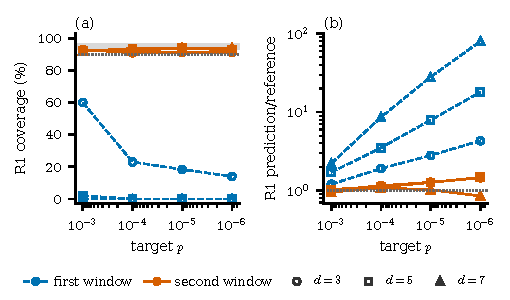
\includegraphics[width=0.38\textwidth]{figs/fig4_windows}
\caption{The free-exponent fit R1 on the two windows. (a) Coverage of the reference by the reported 95\% interval; the grey band is 93--97\% and the dotted line 90\%. (b) Median prediction divided by reference. Open symbols and dashed lines: first window. Filled symbols and solid lines: second window. Circles, squares and triangles are $d=3,5,7$.}\label{fig:win}
\end{figure}

\bibliography{refs}
\end{document}
